\section*{Desarrollo demostrativo del núcleo común}
\addcontentsline{toc}{section}{Desarrollo demostrativo del núcleo común}

Las construcciones siguientes desarrollan las reglas de emisión, el calendario
con memoria, las sucesiones compatibles, la completación cúbica, los lectores
regionales y la reversibilidad del registro dodecafásico. Sus definiciones y
demostraciones preceden a las aplicaciones aritméticas y espectrales que las
utilizan. Los fragmentos procedentes del artículo I conservan sus enunciados,
pruebas y localizadores; el manifiesto de fuentes identifica los componentes,
intervalos y huellas correspondientes.

Las menciones a alfa y al corredor excepcional precisan la procedencia de los
objetos. Las identificaciones posteriores con códigos y retículos no intervienen
en las pruebas espectrales de este manuscrito. Las remisiones al artículo I
documentan esa procedencia, mientras que los argumentos necesarios se presentan
aquí íntegramente. Los censos finitos y las reconstrucciones se interpretan con
las reglas, dominios y coordenadas de partida de cada enunciado; su incorporación
no altera el alcance de la positividad global declarado en el resumen.

% BEGIN NUCLEO_ADITIVO_20260921_CENSO
\clearpage
\section{Núcleo topológico de fase y generación del catálogo de semillas}
\label{act21:tpk:capitulo}

Las dos evaluaciones de APP adquieren eficacia generativa cuando se especifica
qué evaluación actúa, en qué posición se efectúa, cómo se desplaza esa posición
y qué información conserva cada transición. El \emph{Topological Phase Kernel},
abreviado TPK y denominado en español \emph{núcleo topológico de fase}, reúne
estas operaciones en una dinámica sobre estados enriquecidos. Su definición
comprende selección, transporte, actualización aritmética y conservación del
registro. La construcción finita desarrollada en este capítulo proporciona
las semillas sobre las que actuarán las elevaciones regionales y la prolongación
coinductiva.

El resultado principal de esta etapa es un catálogo generado y clasificado:
las condiciones iniciales de los dos cursores producen emisiones enteras;
su lectura ternaria determina palabras orientadas; la acción diedral organiza
esas palabras en órbitas. Cada paso conserva sus preimágenes y las relaciones
que permiten regresar a la descripción precedente. La cadena de cardinales
\[
 104\,976\longrightarrow468\longrightarrow243\subset729,
 \qquad 243\longrightarrow43,
\]
abrevia objetos diferentes. A continuación se construye cada objeto y se
justifica cada recuento, antes de utilizar cualquiera de ellos como dato de
la selección regional.

\subsection{Selección de fase, transporte y estado enriquecido}
\label{act21:tpk:operaciones}

\subsubsection{Selector trítico de fase operativa}

La fase nonádica toma sus valores en \(D_9=\{1,\ldots,9\}\). El selector
trítico es la función
\begin{equation}
 M_{\mathrm{ph}}:D_9\longrightarrow\{-1,0,+1\},\qquad
 M_{\mathrm{ph}}(g)=
 \begin{cases}
 +1,&g\in\{1,4,7\},\\
 -1,&g\in\{2,5,8\},\\
 0,&g\in\{3,6,9\}.
 \end{cases}
 \label{act21:tpk:selector}
\end{equation}
En la realización emisora, el valor \(+1\) activa la evaluación aditiva,
\(-1\) activa la evaluación multiplicativa y \(0\) registra el evento
neutral. La orientación cardinal del cursor es otra coordenada del estado.
Esta separación permite fijar simultáneamente qué operación se lee y en qué
dirección se transporta su punto de evaluación.

Para las transiciones numeradas por \(t\geq1\), la fase previa a la lectura es
\begin{equation}
 g_t=1+[(t-1)]_9,\qquad \epsilon_t=M_{\mathrm{ph}}(g_t),
 \label{act21:tpk:fase}
\end{equation}
donde \([n]_b\) designa el representante de \(n\) módulo \(b\) en
\(\{0,\ldots,b-1\}\). Una ventana de nueve transiciones contiene la sucesión
\((+1,-1,0,+1,-1,0,+1,-1,0)\).

\subsubsection{Cursores orientados y transporte cardinal}

Se utilizan índices \(I_9=\{0,\ldots,8\}\) para las posiciones y etiquetas
positivas \((a,b)=(i+1,j+1)\) para las evaluaciones APP. Un cursor finito es
\[
 c=(i,j;d)\in\mathcal S:=I_9^2\times\mathcal D,
 \qquad \mathcal D=\{N,E,S,O\}.
\]
Las cuatro direcciones actúan mediante
\[
 v_N=(-1,0),\quad v_E=(0,1),\quad
 v_S=(1,0),\quad v_O=(0,-1).
\]
La aplicación cardinal correspondiente a \(d\) es
\[
 T_d(i,j)=\bigl([i+(v_d)_1]_9,[j+(v_d)_2]_9\bigr).
\]
Así, \(M_{\mathrm{ph}}\) y \(T_d\) tienen dominios, codominios y acciones
diferentes. La activación trítica selecciona uno de los dos cursores;
el transporte cardinal modifica su posición en la dirección que ese cursor
ya conserva.

El levantamiento entero del cursor es
\(\widetilde c=(x,y;d)\in\mathbb Z^2\times\mathcal D\), con posición finita
\(([x]_9,[y]_9)\). Sus números de vuelta se recuperan en
\begin{equation}
 x=9\lfloor x/9\rfloor+[x]_9,\qquad
 y=9\lfloor y/9\rfloor+[y]_9.
 \label{act21:tpk:vueltas}
\end{equation}
Estas dos divisiones conciernen al transporte espacial. La división de una
evaluación aditiva o multiplicativa constituye un registro aritmético
distinto, que se conservará junto a ellas.

\subsubsection{Composición de la transición}

El estado de la realización finita incluye los dos cursores levantados,
sus direcciones, la fase, los acumuladores de la ventana activa, la lista
ordenada de bloques ya emitidos y el registro de transiciones. Cada registro
local contiene las posiciones previas, las evaluaciones enteras de ambas
hojas, sus residuos y cocientes, el régimen activo y las orientaciones.
Los campos de prefijo y frontera que aparezcan en una prolongación se
incorporarán al mismo estado con sus reglas de compatibilidad.

La transición se ordena como
\begin{equation}
 \mathcal U_t=\mathsf{Mem}_t\circ\mathsf{Tra}_t\circ\mathsf{Sel}_t.
 \label{act21:tpk:composicion}
\end{equation}
La selección determina el régimen y conserva la muestra previa a todo
desplazamiento. El transporte aplica el movimiento activo y la inversión
cardinal prescrita por el calendario. La actualización incorpora esa muestra
a los acumuladores y al registro; al terminar una ventana, emite su bloque.
La composición utiliza por tanto una muestra anterior al transporte aunque
su archivo definitivo se efectúe al final de la transición.

\subsection{Condiciones iniciales y enumeración reversible}
\label{act21:tpk:semillas}

Las hojas aditiva y multiplicativa disponen de cursores independientes. El
dominio de condiciones iniciales es el producto ordenado
\[
 \Omega_{\mathrm{seed}}=\mathcal S_+\times\mathcal S_\times,
 \qquad |\mathcal S|=9^2\cdot4=324.
\]
Por consiguiente,
\begin{equation}
 |\Omega_{\mathrm{seed}}|=324^2=104\,976.
 \label{act21:tpk:censo-inicial}
\end{equation}
El número \(81\) cuenta posiciones; \(324\) cuenta posiciones orientadas
de un cursor; \(104\,976\) cuenta parejas ordenadas de cursores. La elección
de una posición en APP conserva únicamente una parte de una condición
inicial del emisor.

Se fija la numeración
\[
 \operatorname{ind}(N)=0,\quad\operatorname{ind}(E)=1,\quad
 \operatorname{ind}(S)=2,\quad\operatorname{ind}(O)=3,
\]
y se define
\begin{equation}
 \nu(i,j;d)=4(9i+j)+\operatorname{ind}(d).
 \label{act21:tpk:indice-semilla}
\end{equation}

\begin{proposition}[Enumeración exacta de las condiciones iniciales]
\label{act21:tpk:enumeracion}
La aplicación \(\nu\) es una biyección de \(\mathcal S\) sobre
\(\{0,\ldots,323\}\). La pareja de índices se codifica de manera reversible
por \(324\nu_++\nu_\times\in\{0,\ldots,104\,975\}\).
\end{proposition}
\begin{proof}
La división por cuatro recupera
\[
 \operatorname{ind}(d)=[\nu]_4,\qquad
 j=[\lfloor\nu/4\rfloor]_9,\qquad i=\lfloor\nu/36\rfloor.
\]
Las cotas del dominio garantizan que estas tres cantidades pertenecen a
sus conjuntos de índices y reconstruyen \(\nu\) mediante
\eqref{act21:tpk:indice-semilla}. Para la pareja, la división euclídea por
\(324\) recupera cociente \(\nu_+\) y residuo \(\nu_\times\).
\end{proof}

La enumeración recorre el dominio completo antes de cualquier agrupación
regional. Los índices se utilizan para localizar las preimágenes de una
emisión, manteniendo explícita la condición que produjo cada trayectoria.

\subsection{Evaluación de las hojas y registro aritmético}
\label{act21:tpk:lecturas}

En una posición positiva \((a,b)\), las evaluaciones enteras son
\(A_+(a,b)=a+b\) y \(A_\times(a,b)=ab\). Para \(n>0\), se mantienen
\begin{equation}
 \rho_9(n)=1+[n-1]_9,\qquad
 q_9(n)=\lfloor(n-1)/9\rfloor,\qquad
 n=\rho_9(n)+9q_9(n).
 \label{act21:tpk:division-evaluacion}
\end{equation}
La activación aditiva incorpora \(\rho_9(A_+)\) al acumulador
correspondiente. La activación multiplicativa utiliza un observable del
residuo \(\rho_9(A_\times)\), definido a continuación.

\subsubsection{Exponente discreto en las unidades módulo nueve}

Las potencias de \(2\) módulo \(9\) recorren
\[
 2^0,2^1,\ldots,2^5\equiv1,2,4,8,7,5\pmod9,
 \qquad 2^6\equiv1\pmod9.
\]
El logaritmo discreto en este grupo de seis unidades se representa por
\begin{equation}
 \ell_9(1)=0,\quad\ell_9(2)=1,\quad\ell_9(4)=2,
 \quad\ell_9(8)=3,\quad\ell_9(7)=4,\quad\ell_9(5)=5.
 \label{act21:tpk:logaritmo}
\end{equation}
La ley emisora extiende el observable mediante
\(\ell_9(3)=\ell_9(6)=\ell_9(9)=0\). Para conservar su procedencia, la
muestra registrada incluye el residuo original y el indicador de pertenencia
al grupo de unidades. De ese modo, un valor observado cero puede proceder
de la unidad \(1\) o de alguno de los tres residuos no invertibles, y su
origen permanece recuperable.

\subsubsection{Orden de lectura y movimiento}

Las evaluaciones se efectúan en las posiciones anteriores a la transición.
Si \(\epsilon_t=+1\), se acumula la lectura aditiva y se desplaza su cursor.
Si \(\epsilon_t=-1\), se acumula el exponente discreto multiplicativo y se
desplaza el segundo cursor. Si \(\epsilon_t=0\), se incrementa el contador
neutral y se conservan ambas posiciones.

Al finalizar los pasos \(27\) y \(54\), las dos direcciones se sustituyen
por sus opuestas. Las ventanas se encadenan conservando posiciones y
orientaciones. Al inicio de cada ventana sólo se ponen a cero sus tres
acumuladores locales; el registro anterior permanece disponible.

\begin{proposition}[Inversión del transporte levantado]
\label{act21:tpk:inversion}
Sean \(a,b\in\{0,1\}\) los indicadores de activación e inversión de un
cursor. Si \(\operatorname{opp}\) intercambia \(N\leftrightarrow S\) y
\(E\leftrightarrow O\), la transformación
\[
 F_{a,b}(z,d)=\bigl(z+a v_d,\operatorname{opp}^{\,b}(d)\bigr)
\]
tiene inversa
\[
 F_{a,b}^{-1}(z',d')=
 \bigl(z'-a v_{\operatorname{opp}^{\,b}(d')},
       \operatorname{opp}^{\,b}(d')\bigr).
\]
La reducción espacial módulo nueve entrelaza esta transformación con el
transporte finito.
\end{proposition}
\begin{proof}
Aplicar dos veces la oposición recupera la dirección inicial. Una vez
recuperada esa dirección, la resta de \(a v_d\) deshace el desplazamiento.
Para la proyección espacial basta la igualdad
\([z+a v_d]_9=[[z]_9+a v_d]_9\), componente a componente. La inversión de
dirección conserva esta igualdad.
\end{proof}

La fase determina los indicadores utilizados por la inversa. El registro
espacial y el aritmético pueden así conservarse conjuntamente, incluso al
atravesar el borde del representante \(I_9^2\).

\subsection{Seis ventanas y emisión decimal por bloques}
\label{act21:tpk:emision}

\subsubsection{Acumulación en una ventana nonádica}

La ventana \(m\), con \(1\leq m\leq6\), comprende los pasos
\(9m-8,\ldots,9m\). Sean \(S_m\) la suma de sus residuos positivos
aditivos activos, \(E_m\) la suma de sus exponentes discretos activos y
\(Z_m\) su número de eventos neutrales.

\begin{lemma}[Multiplicidades de activación]
\label{act21:tpk:tres-eventos}
Cada ventana contiene tres activaciones aditivas, tres multiplicativas y
tres neutrales. En particular, \(Z_m=3\).
\end{lemma}
\begin{proof}
Las fases de una ventana recorren exactamente \(1,\ldots,9\). Cada uno
de los tres conjuntos de \eqref{act21:tpk:selector} tiene cardinal tres.
\end{proof}

Las seis ventanas forman \(54\) transiciones y producen seis bloques.
Esta longitud pertenece al emisor inicial aquí definido. La continuación
en profundidad actúa después sobre las palabras y sus registros compatibles.

\subsubsection{Regla de codificación decimal}

La ley emisora especifica las cifras
\begin{align}
 d_{m,1}&=[S_m]_{10},\notag\\
 d_{m,2}&=[S_m+E_m]_{10},\notag\\
 d_{m,3}&=[3S_m+5E_m+7Z_m]_{10},\notag\\
 U_m&=100d_{m,1}+10d_{m,2}+d_{m,3}.
 \label{act21:tpk:bloque-decimal}
\end{align}
Los pesos \(100,10,1\) son las posiciones centena, decena y unidad.
El subíndice \(10\) indica el residuo decimal, y cada bloque satisface
\(0\leq U_m\leq999\). La palabra emitida es la sucesión ordenada
\(\mathbf U=(U_1,\ldots,U_6)\), con ancho fijo de tres cifras por bloque.

Los coeficientes \(3,5,7\) constituyen los pesos explícitos de esta ley
emisora. Una vez fijada la regla, cada cifra se calcula a partir de los
acumuladores, y los resultados de este capítulo se deducen de esa regla.
El número \(1\) que aparece en su forma reducida tiene una procedencia
adicional concreta: \(7Z_m=21\equiv1\pmod{10}\).

Si \(s_m=[S_m]_{10}\) y \(e_m=[E_m]_{10}\), se obtiene
\begin{equation}
 G(s_m,e_m)=100s_m+10[s_m+e_m]_{10}
                   +[3s_m+5e_m+1]_{10}=U_m.
 \label{act21:tpk:acoplamiento-firmas}
\end{equation}
La letra \(e_m\) denota aquí una componente de la firma de exponentes
discretos. Su definición pertenece al emisor finito.

\begin{proposition}[Recuperación de las dos firmas]
\label{act21:tpk:recuperacion-firmas}
La aplicación \(G:\{0,\ldots,9\}^2\to\{0,\ldots,999\}\) es inyectiva.
Para un bloque \(U=100a+10b+c\) de su imagen, la inversa es
\[
 s=a,\qquad e=[b-a]_{10},\qquad
 c=[3s+5e+1]_{10}.
\]
En consecuencia, la palabra \(\mathbf U\) determina las dos firmas de
seis componentes \(\mathbf s\) y \(\mathbf e\).
\end{proposition}
\begin{proof}
Los dos últimos sumandos de \eqref{act21:tpk:acoplamiento-firmas} pertenecen a
\(\{0,\ldots,99\}\), de modo que la centena recupera \(s\). La decena
es \([s+e]_{10}\); al restar \(s\) y reducir módulo diez se recupera
\(e\). La unidad verifica la tercera congruencia. La reconstrucción se
aplica independientemente a las seis posiciones de la palabra.
\end{proof}

Los totales enteros \(S_m,E_m\) se recuperan de las lecturas registradas;
las centenas y decenas recuperan sus residuos. Por ejemplo, un total
\(S_m=15\) produce \(s_m=5\). Esta diferencia identifica exactamente
qué información conserva cada nivel de codificación.

\subsubsection{Codificación posicional de la palabra de seis bloques}

Los seis bloques admiten una codificación entera de ancho fijo,
\begin{equation}
 \mathscr N(\mathbf U)=\sum_{m=1}^{6}U_m1000^{6-m},
 \qquad0\leq\mathscr N(\mathbf U)<1000^6.
 \label{act21:tpk:entero-base1000}
\end{equation}
El primer bloque ocupa la posición de mayor peso y el sexto, la de unidades
de base mil. Un bloque \(058\) ocupa una posición completa con valor
entero \(58\); su ancho de tres cifras forma parte de la presentación
decimal de esa posición.

\begin{proposition}[Recuperación posicional de las emisiones]
\label{act21:tpk:inversa-base1000}
La codificación \eqref{act21:tpk:entero-base1000} determina la palabra completa
mediante
\[
 U_m=\left[\left\lfloor
 \frac{\mathscr N(\mathbf U)}{1000^{6-m}}\right\rfloor\right]_{1000},
 \qquad1\leq m\leq6.
\]
\end{proposition}
\begin{proof}
Al dividir por \(1000^{6-m}\), los bloques anteriores producen múltiplos
enteros de \(1000\), el bloque \(m\) produce \(U_m\), y la contribución
de los posteriores pertenece a \([0,1)\). La parte entera elimina esta
última contribución y el residuo módulo \(1000\) elimina las primeras.
\end{proof}

Esta codificación conserva las seis emisiones. Su dominio posee posiciones
ordenadas de base mil, mientras el dominio APP posee posiciones espaciales
módulo nueve. La composición mantiene ambos índices: \(m\) identifica una
ventana de emisión y \((i,j)\) identifica la celda visitada durante una
transición de esa ventana.

\subsection{Cálculo completo de una emisión que comienza por 501}
\label{act21:tpk:ejemplo501}

Se fijan las condiciones iniciales
\[
 c_{+,0}=(0,4;N),\qquad c_{\times,0}=(2,3;N),
 \qquad \nu_+=16,\quad\nu_\times=84.
\]
Las posiciones positivas iniciales son \((1,5)\) y \((3,4)\). El índice
cronológico previo es \(t=0\), la primera fase leída es \(g_1=1\) y el
registro está vacío. Estas coordenadas son las entradas
del cálculo; los bloques se obtienen ejecutando la recurrencia.

\begin{table}[htbp]
\caption{Primera ventana: lecturas previas y acumulación activa.}
\label{act21:tpk:tabla-501}
\small
\begin{tabular}{@{}rcccrrr@{}}
\toprule
\(t\)&\(\epsilon_t\)&posición \(+\)&posición \(\times\)&
\(\Delta S\)&\(\Delta E\)&\((S,E,Z)\)\\
\midrule
1&\(+1\)&\((1,5)\)&\((3,4)\)&6&0&\((6,0,0)\)\\
2&\(-1\)&\((9,5)\)&\((3,4)\)&0&0&\((6,0,0)\)\\
3&0&\((9,5)\)&\((2,4)\)&0&0&\((6,0,1)\)\\
4&\(+1\)&\((9,5)\)&\((2,4)\)&5&0&\((11,0,1)\)\\
5&\(-1\)&\((8,5)\)&\((2,4)\)&0&3&\((11,3,1)\)\\
6&0&\((8,5)\)&\((1,4)\)&0&0&\((11,3,2)\)\\
7&\(+1\)&\((8,5)\)&\((1,4)\)&4&0&\((15,3,2)\)\\
8&\(-1\)&\((7,5)\)&\((1,4)\)&0&2&\((15,5,2)\)\\
9&0&\((7,5)\)&\((9,4)\)&0&0&\((15,5,3)\)\\
\bottomrule
\end{tabular}
\notatabla{Las posiciones son etiquetas positivas de las celdas anteriores
al movimiento. Los eventos neutrales incrementan únicamente \(Z\).}
\end{table}

Las tres evaluaciones aditivas activas son
\[
 1+5=6,\qquad9+5=14=5+9,\qquad8+5=13=4+9,
\]
de modo que \(S_1=6+5+4=15\). Las tres evaluaciones multiplicativas activas
son \(3\cdot4=12\), \(2\cdot4=8\) y \(1\cdot4=4\). Sus residuos
positivos son \(3,8,4\), con observables \(0,3,2\); por tanto,
\(E_1=5\). Finalmente \(Z_1=3\). La regla decimal da
\[
 d_{1,1}=[15]_{10}=5,\quad
 d_{1,2}=[15+5]_{10}=0,\quad
 d_{1,3}=[45+25+21]_{10}=1,
\]
y se obtiene \(U_1=501\).

La segunda lectura aditiva anterior tiene cociente aritmético \(1\),
mientras su cursor levantado está en \((-1,4;N)\), con número de vuelta
vertical \(-1\). Son dos datos diferentes del mismo registro. Ambos
intervienen en la recuperación íntegra de la evaluación y de su posición.

\begin{table}[htbp]
\caption{Las seis ventanas de la condición inicial \((16,84)\).}
\label{act21:tpk:tabla-seis501}
\begin{tabular}{@{}rrrrrrrr@{}}
\toprule
\(m\)&pasos&\(S_m\)&\(E_m\)&\(Z_m\)&\(s_m\)&\(U_m\)&\([-U_m]_3\)\\
\midrule
1&1--9&15&5&3&5&501&0\\
2&10--18&6&5&3&6&614&1\\
3&19--27&24&5&3&4&498&0\\
4&28--36&21&5&3&1&169&2\\
5&37--45&12&5&3&2&272&1\\
6&46--54&12&5&3&2&272&1\\
\bottomrule
\end{tabular}
\end{table}

La palabra resultante y sus firmas son
\begin{align*}
 \mathbf U&=(501,614,498,169,272,272),\\
 \mathbf s&=(5,6,4,1,2,2),&
 \mathbf e&=(5,5,5,5,5,5).
\end{align*}
La inversión cardinal tras el paso \(27\) modifica los recorridos de las
tres ventanas finales. El bloque repetido \(272\) corresponde a dos
ventanas sucesivas con posiciones y registro cronológico propios.

Como segundo caso, la condición inicial mínima \((\nu_+,\nu_\times)=(0,0)\)
produce
\[
 \mathbf U=(252,109,252,903,850,850),\quad
 \mathbf s=(2,1,2,9,8,8),\quad
 \mathbf e=(3,9,3,1,7,7).
\]
En este caso, ambos cursores regresan a su posición y orientación iniciales
tras \(54\) transiciones. La fase nonádica completa seis vueltas, el
contador cronológico avanza \(54\) unidades y el registro contiene
\(54\) muestras. La lectura posicional del retorno y
la historia registrada describen propiedades distintas de la ejecución.

\subsection{Factorización del censo finito}
\label{act21:tpk:censo}

Las firmas \(f_+(\nu)=\mathbf s\) y \(f_\times(\nu)=\mathbf e\) se
calculan ejecutando el cursor correspondiente durante las seis ventanas.
La independencia de posiciones y direcciones entre los dos cursores da
\begin{equation}
 T_{\mathrm{em}}(\nu_+,\nu_\times)
   =G^{(6)}\bigl(f_+(\nu_+),f_\times(\nu_\times)\bigr),
 \label{act21:tpk:factorizacion}
\end{equation}
donde \(G^{(6)}\) aplica \eqref{act21:tpk:acoplamiento-firmas} en cada posición.
La factorización permite enumerar primero \(324+324\) trayectorias y
combinar después las firmas distintas, conservando la multiplicidad de
sus preimágenes.

\par\noindent\begin{minipage}{\linewidth}
\subsubsection{Imágenes de las dos firmas}

Las tablas siguientes incluyen todas las firmas. Su multiplicidad es el
número de condiciones iniciales que las producen; el índice mínimo localiza
una de esas condiciones. La preimagen completa se define por
\[
 f_\sigma^{-1}(a)=\{\nu\in\{0,\ldots,323\}:f_\sigma(\nu)=a\}.
\]
La recurrencia de las secciones anteriores determina cada elemento de este
conjunto mediante un cálculo entero finito.

\begin{table}[H]
\centering\fontsize{9.5}{11.4}\selectfont
\setlength{\abovecaptionskip}{8pt}\setlength{\belowcaptionskip}{6pt}
\renewcommand{\arraystretch}{1.12}
\caption{Las dieciocho firmas aditivas.}
\label{act21:tpk:firmas-aditivas}
\begin{tabular}{@{}lrr@{\qquad}lrr@{}}
\toprule
firma&multiplicidad&\(\nu_{\min}\)&firma&multiplicidad&\(\nu_{\min}\)\\
\midrule
\texttt{122564}&18&17&\texttt{564122}&18&16\\
\texttt{122898}&18&24&\texttt{645212}&18&4\\
\texttt{212645}&18&5&\texttt{654889}&18&33\\
\texttt{212988}&18&0&\texttt{889221}&18&13\\
\texttt{221456}&18&29&\texttt{889654}&18&32\\
\texttt{221889}&18&12&\texttt{898122}&18&25\\
\texttt{456221}&18&28&\texttt{898465}&18&20\\
\texttt{465898}&18&21&\texttt{988212}&18&1\\
\texttt{546988}&18&9&\texttt{988546}&18&8\\
\bottomrule
\end{tabular}

\par\vspace{12pt}

\caption{Las veintiséis firmas multiplicativas.}
\label{act21:tpk:firmas-multiplicativas}
\begin{tabular}{@{}lrr@{\qquad}lrr@{}}
\toprule
firma&multiplicidad&\(\nu_{\min}\)&firma&multiplicidad&\(\nu_{\min}\)\\
\midrule
\texttt{000000}&108&8&\texttt{555555}&24&84\\
\texttt{177393}&8&1&\texttt{555717}&8&14\\
\texttt{177555}&8&54&\texttt{555771}&8&18\\
\texttt{177771}&8&11&\texttt{555933}&8&24\\
\texttt{339555}&8&6&\texttt{717555}&8&12\\
\texttt{339771}&8&15&\texttt{717717}&8&21\\
\texttt{339933}&8&59&\texttt{717933}&8&19\\
\texttt{393177}&8&0&\texttt{771177}&8&9\\
\texttt{393393}&8&45&\texttt{771339}&8&13\\
\texttt{393555}&8&40&\texttt{771555}&8&16\\
\texttt{555177}&8&52&\texttt{933339}&8&57\\
\texttt{555339}&8&4&\texttt{933555}&8&26\\
\texttt{555393}&8&41&\texttt{933717}&8&17\\
\bottomrule
\end{tabular}
\end{table}
\end{minipage}\par


\begin{proposition}[Imagen y multiplicidades del emisor]
\label{act21:tpk:468}
La imagen \(\mathcal U_6=\operatorname{im}T_{\mathrm{em}}\) contiene
\(468\) palabras distintas. Sus preimágenes se distribuyen en \(432\)
fibras de cardinal \(144\), \(18\) de cardinal \(432\) y \(18\) de
cardinal \(1944\).
\end{proposition}
\begin{proof}
La evaluación exhaustiva del algoritmo de la sección~\ref{act21:tpk:algoritmo}
sobre los índices \(0,\ldots,323\) da las dos tablas anteriores.
La primera partición tiene \(18\) clases de cardinal \(18\), y la segunda
\(24\) clases de cardinal \(8\), una de cardinal \(24\) y una de
cardinal \(108\). Las sumas \(18\cdot18=324\) y
\(24\cdot8+24+108=324\) comprueban la masa total de ambas particiones.
La proposición~\ref{act21:tpk:recuperacion-firmas} hace inyectivo el acoplamiento
de sus imágenes; por tanto, hay \(18\cdot26=468\) emisiones.
Por \eqref{act21:tpk:factorizacion}, la preimagen de una pareja de firmas es
el producto de sus dos preimágenes. Se obtienen \(18\cdot24=432\)
productos de cardinal \(18\cdot8=144\), \(18\) de cardinal
\(18\cdot24=432\) y \(18\) de cardinal \(18\cdot108=1944\).
Finalmente,
\[
 432\cdot144+18\cdot432+18\cdot1944=104\,976.
\]
La parte enumerativa es una comprobación finita exacta de la recurrencia;
la factorización explica por qué ese recuento cubre todas las parejas.
\end{proof}

La emisión del ejemplo \ref{act21:tpk:ejemplo501} tiene una fibra de cardinal
\(18\cdot24=432\). El ejemplo de índices \((0,0)\) tiene una fibra de
cardinal \(18\cdot8=144\). En ambos casos la palabra emitida recupera
las firmas, mientras la identificación de una condición inicial particular
utiliza su índice o su registro de trayectoria.

\subsection{Lectura ternaria orientada y conservación de las fibras}
\label{act21:tpk:reduccion-ternaria}

La reducción orientada actúa separadamente sobre cada bloque:
\begin{equation}
 \Psi:\mathcal U_6\longrightarrow\mathbb F_3^6,\qquad
 \Psi(U_1,\ldots,U_6)=([-U_1]_3,\ldots,[-U_6]_3).
 \label{act21:tpk:psi}
\end{equation}
Su signo fija una orientación del catálogo. La identificación balanceada
\(0\mapsto0\), \(1\mapsto+1\), \(2\mapsto-1\) se aplica después,
componente a componente.

El módulo nueve organiza las evaluaciones y posiciones de APP; los residuos
módulo diez forman cada cifra; la base mil reúne tres posiciones decimales;
el módulo tres determina la firma ternaria de cada bloque. Estos cuatro usos
tienen objetos y funciones definidos. En particular, \(\Psi\) lee seis
bloques y produce seis trits; una conversión posicional del entero formado
por dieciocho cifras sería otra operación.

Para las dos condiciones calculadas se obtiene
\begin{align*}
 \Psi(501,614,498,169,272,272)&=(0,1,0,2,1,1),\\
 \Psi(252,109,252,903,850,850)&=(0,2,0,0,2,2).
\end{align*}
El emisor decimal está definido antes de esta reducción. La función de
\(\Psi\) es producir el objeto ternario sobre el que actúan la simetría
orbital y los selectores regionales. Esa función explica su posición en la
genealogía: enlaza una emisión ya calculada con una clasificación estructural.

La imagen \(\mathcal W_6:=\Psi(\mathcal U_6)\) contiene exactamente
\(243\) palabras dentro del conjunto ambiente de \(3^6=729\) palabras.
La enumeración del algoritmo final da el histograma
\begin{equation}
\begin{array}{c|rrrrrr}
 |\Psi^{-1}(w)|&1&2&3&4&5&6\\\hline
 \text{número de palabras }w&132&66&18&3&6&18.
\end{array}
\label{act21:tpk:fibras-ternarias}
\end{equation}
Las sumas de ambas lecturas son
\[
132+66+18+3+6+18=243,
\qquad132+2\cdot66+3\cdot18+4\cdot3+5\cdot6+6\cdot18=468.
\]
La primera cuenta palabras ternarias; la segunda recupera el número de
emisiones distribuidas entre sus fibras.

\begin{example}[Dos emisiones con la misma firma ternaria]
\label{act21:tpk:colision}
Las emisiones
\[
 (498,501,614,252,252,109),\qquad
 (870,810,923,252,252,109)
\]
son distintas y ambas tienen imagen \((0,0,1,0,0,2)\) por \(\Psi\).
Cada una tiene \(144\) condiciones iniciales. La palabra ternaria conserva
una clase de lectura; las emisiones y sus preimágenes distinguen los datos
que confluyen en esa clase.
\end{example}

La conservación de fibras se expresa concretamente mediante
\[
 \mathcal F_w=\{\mathbf U\in\mathcal U_6:\Psi(\mathbf U)=w\},
 \qquad
 \Omega_{\mathbf U}=T_{\mathrm{em}}^{-1}(\mathbf U).
\]
Por tanto, la preimagen completa de \(w\) en el dominio inicial es la
unión disjunta de los conjuntos \(\Omega_{\mathbf U}\), con
\(\mathbf U\in\mathcal F_w\). El registro enriquecido puede conservar la
emisión, sus firmas y la condición inicial junto a su lectura ternaria.
La inversa exacta se refiere entonces al dato registrado con su tipo;
la palabra de seis trits aislada mantiene el alcance preciso de
\eqref{act21:tpk:psi}.

\subsection{Acción diedral y las cuarenta y tres órbitas}
\label{act21:tpk:orbitas}

Sobre seis coordenadas se definen las permutaciones
\begin{align}
 r(u_1,u_2,u_3,u_4,u_5,u_6)
   &=(u_3,u_1,u_2,u_5,u_6,u_4),\\
 s(u_1,u_2,u_3,u_4,u_5,u_6)
   &=(u_4,u_5,u_6,u_1,u_2,u_3).
 \label{act21:tpk:generadores-diedrales}
\end{align}
La primera rota los dos grupos de tres coordenadas con sentidos conjugados;
la segunda intercambia ambos grupos. Su composición satisface
\(r^3=s^2=1\) y \(srs=r^{-1}\). Generan así una acción del grupo diedral
\(D_3\), de seis elementos.

\begin{proposition}[Equivariancia y estabilidad del catálogo]
\label{act21:tpk:equivarianza}
La reducción \(\Psi\) conmuta con la acción de \(D_3\). Los conjuntos
\(\mathcal U_6\) y \(\mathcal W_6\) son estables bajo sus generadores.
\end{proposition}
\begin{proof}
La igualdad \(\Psi(g\mathbf U)=g\Psi(\mathbf U)\) se verifica en cada
coordenada porque \(g\) permuta posiciones y \(\Psi\) aplica la misma
reducción a cada posición. La estabilidad del catálogo constituye otra
comprobación: al generar sus \(468\) elementos mediante
\eqref{act21:tpk:factorizacion}, se verifica que \(r\mathbf U\) y
\(s\mathbf U\) pertenecen de nuevo a ese conjunto. El algoritmo de la
sección~\ref{act21:tpk:algoritmo} efectúa estas comprobaciones de pertenencia.
La equivariancia transmite después la estabilidad a su imagen ternaria.
\end{proof}

\begin{proposition}[Descomposición orbital completa]
\label{act21:tpk:43}
El conjunto \(\mathcal W_6\) se descompone en \(43\) órbitas: \(38\)
de cardinal seis y \(5\) de cardinal tres.
\end{proposition}
\begin{proof}
Para cada \(w\in\mathcal W_6\) se forma
\[
 \mathcal O(w)=\{w,rw,r^2w,sw,srw,sr^2w\}.
\]
Se escoge como representante la palabra lexicográficamente mínima de ese
conjunto. Dos palabras tienen el mismo representante exactamente cuando
pertenecen a la misma órbita. El algoritmo genera la lista de representantes
de la tabla~\ref{act21:tpk:representantes}; sus cardinales suman
\(38\cdot6+5\cdot3=243\). Como cada palabra del catálogo participa en
esta operación y el catálogo es estable, la lista cubre toda la imagen.
\end{proof}

\begin{table}[htbp]
\caption{Representantes mínimos y cardinales de las cuarenta y tres órbitas.}
\label{act21:tpk:representantes}
\small
\begin{tabular}{@{}lr@{\qquad}lr@{\qquad}lr@{}}
\toprule
representante&cardinal&representante&cardinal&representante&cardinal\\
\midrule
\texttt{001002}&6&\texttt{002112}&6&\texttt{012222}&6\\
\texttt{001011}&6&\texttt{002211}&6&\texttt{021022}&6\\
\texttt{001012}&6&\texttt{002220}&6&\texttt{021121}&6\\
\texttt{001021}&6&\texttt{011021}&6&\texttt{021202}&6\\
\texttt{001022}&6&\texttt{011112}&6&\texttt{022022}&3\\
\texttt{001100}&3&\texttt{011120}&6&\texttt{022112}&6\\
\texttt{001101}&6&\texttt{011201}&6&\texttt{022121}&6\\
\texttt{001110}&6&\texttt{011211}&6&\texttt{022202}&3\\
\texttt{001112}&6&\texttt{011220}&6&\texttt{022211}&6\\
\texttt{001202}&6&\texttt{011222}&6&\texttt{022222}&6\\
\texttt{001210}&6&\texttt{012112}&6&\texttt{112112}&3\\
\texttt{001211}&6&\texttt{012121}&6&\texttt{112211}&3\\
\texttt{001220}&6&\texttt{012202}&6&\texttt{112222}&6\\
\texttt{001222}&6&\texttt{012210}&6&&\\
\texttt{002012}&6&\texttt{012220}&6&&\\
\bottomrule
\end{tabular}
\end{table}

Las órbitas heredan invariantes enteros de sus fibras. Para cada palabra,
\(n(w)=|\mathcal F_w|\) cuenta emisiones, mientras
\[
 M(w)=\sum_{\mathbf U\in\mathcal F_w}|\Omega_{\mathbf U}|
\]
cuenta condiciones iniciales. El censo de símbolos
\(c(w)=(n_0,n_1,n_2)\) registra cuántas veces aparece cada clase ternaria.
Estos datos, junto con la orientación y el soporte de los recorridos,
proporcionan los predicados de la selección regional posterior. La
clasificación conserva así más información que la forma de una palabra
representante.

\subsection{Algoritmo autocontenido de enumeración y control}
\label{act21:tpk:algoritmo}

La enumeración utiliza enteros, listas finitas y las operaciones ya definidas.
El siguiente procedimiento precisa su ejecución; \(\sigma\) toma los valores
\(+\) y \(\times\).

\begin{enumerate}
\item Para cada \(\nu=0,\ldots,323\), recuperar \((i,j;d)\) mediante
la inversa de \eqref{act21:tpk:indice-semilla}. Iniciar una lista vacía de firmas.
\item Para cada ventana \(m=1,\ldots,6\), iniciar el acumulador \(A=0\).
Recorrer \(t=9m-8,\ldots,9m\), calculando \(\epsilon_t\) por
\eqref{act21:tpk:fase}.
\item Si \(\sigma=+\) y \(\epsilon_t=+1\), añadir
\(\rho_9(i+j+2)\) a \(A\) y actualizar
\((i,j)\leftarrow T_d(i,j)\). Si \(\sigma=\times\) y
\(\epsilon_t=-1\), añadir
\(\ell_9(\rho_9((i+1)(j+1)))\) y efectuar el mismo transporte.
\item Al terminar \(t=27\) o \(t=54\), sustituir \(d\) por su opuesta.
Al concluir la ventana, añadir \([A]_{10}\) a la lista de firmas.
Conservar la posición y la dirección para la siguiente ventana.
\item Agrupar los \(324\) índices por igualdad de sus listas de seis
componentes. Estas dos agrupaciones dan \(f_+\), \(f_\times\) y todas
sus preimágenes.
\item Para cada pareja de firmas distintas, aplicar \(G^{(6)}\).
Asignar a la emisión la multiplicidad producto de las dos preimágenes.
Comprobar la recuperación de firmas en cada bloque y la suma de
multiplicidades \(104\,976\).
\item Aplicar \(\Psi\) a cada emisión y agrupar por igualdad de palabras.
Contar los \(243\) valores y las multiplicidades de
\eqref{act21:tpk:fibras-ternarias}.
\item Aplicar \(r,s\) a cada emisión y verificar pertenencia al catálogo.
Para cada palabra ternaria, formar sus seis imágenes diedrales, eliminar
repeticiones y registrar su mínimo lexicográfico. Contar las \(43\)
órbitas y los dos tamaños de la tabla~\ref{act21:tpk:representantes}.
\end{enumerate}

La ejecución termina: el primer tramo evalúa \(648\) trayectorias de
\(54\) transiciones; el segundo combina \(468\) parejas de firmas; el
tercero agrupa un conjunto de \(243\) palabras. Una comprobación directa
adicional puede ejecutar las \(104\,976\) parejas y contrastar la
factorización \eqref{act21:tpk:factorizacion}; su alcance coincide con el mismo
dominio finito.

\subsection{Conservación del registro y función de las semillas}
\label{act21:tpk:conclusion}

Sea \(\mathsf{Sample}(q_t)\) la muestra previa a la transición y
\(\mathcal M_t\) el registro acumulado. La actualización de memoria es
\begin{equation}
 \mathcal M_{t+1}=\mathcal M_t\mathbin{\Vert}\mathsf{Sample}(q_t),
 \label{act21:tpk:archivo}
\end{equation}
donde \(\Vert\) denota concatenación ordenada. La inducción da
\[
 \mathcal M_n=\mathcal M_0\mathbin{\Vert}
 (\mathsf{Sample}(q_0),\ldots,\mathsf{Sample}(q_{n-1})).
\]
Los acumuladores se reconstruyen sumando las contribuciones activas de
cada segmento de nueve registros. Sus cocientes, las vueltas de los
cursores y las orientaciones permanecen asociados a las mismas transiciones.
La ejecución determina ese registro mediante la recurrencia; el archivo
preserva la procedencia concreta de las lecturas.

Al finalizar esta etapa están construidos el dominio completo de condiciones
iniciales, la emisión decimal, sus dos firmas recuperables, la imagen ternaria,
sus fibras y su clasificación orbital. Los censos \(104\,976\), \(468\),
\(243\), \(729\) y \(43\) tienen ahora dominio y mecanismo de obtención.
Las selecciones regionales recibirán estas estructuras con sus invariantes,
y las elevaciones actuarán sobre palabras orientadas con procedencia
conservada. Esa continuidad convierte el catálogo finito en antecedente
constructivo del desarrollo coinductivo.

% END NUCLEO_ADITIVO_20260921_CENSO
% Fragmento conservado; véase MANIFIESTO_ANTECEDENTES_LECTURA.json.
\section{Desarrollo del núcleo formal: condiciones iniciales, geometría y refinamiento}
\label{sec:extension}

El soporte de ochenta y una posiciones no coincide con el dominio de condiciones iniciales de la dinámica. Una condición inicial debe indicar además una orientación; y las hojas aditiva y multiplicativa disponen de cursores independientes. Esta distinción permite reconstruir exhaustivamente la emisión sin seleccionar de antemano una región numérica.

\subsection{Los estados iniciales y la recurrencia de emisión}

Para la enumeración utilizamos índices \(I_9=\{0,\ldots,8\}\), relacionados con las etiquetas positivas por \(i\mapsto i+1\). Sea
\[
 \mathcal S=I_9^2\times\{N,E,S,O\},\qquad
 \Omega_{\rm seed}=\mathcal S_+\times\mathcal S_\times.
\]
Cada condición inicial \(\omega=(s_+,s_\times)\) determina dos posiciones y dos direcciones. El dominio comprende todas las parejas ordenadas, por lo que
\begin{equation}
 |\mathcal S|=324,\qquad |\Omega_{\rm seed}|=324^2=104\,976.
 \label{eq:semillas}
\end{equation}
El anexo independiente enumera todas estas condiciones; el cuerpo presenta la ley que las transforma. Las filas de una tabla de emisiones son fibras de este dominio de condiciones iniciales.

La realización finita utiliza seis ventanas de nueve transiciones. En cada instante \(t\), la firma de fase es \(M_{\rm ph}(1+((t-1)\bmod9))\). Si vale \(+1\), se lee el residuo positivo \(\Sigma(i+1,j+1)=\rho_9(i+j+2)\) del primer cursor y después se desplaza ese cursor; si vale \(-1\), se lee el residuo positivo \(\Pi(i+1,j+1)=\rho_9((i+1)(j+1))\) del segundo cursor y después se desplaza el segundo. El valor cero incrementa el contador neutral. Al finalizar las transiciones veintisiete y cincuenta y cuatro, se invierten las orientaciones cardinales. Las evaluaciones enteras y sus cocientes se conservan en el registro, pero el emisor utiliza las lecturas residuales aquí especificadas.

En el sector de unidades, el lector multiplicativo utiliza el logaritmo discreto de base dos en \((\ZZ/9\ZZ)^\times\):
\[
 \ell_9(1)=0,\quad\ell_9(2)=1,\quad\ell_9(4)=2,\quad
 \ell_9(8)=3,\quad\ell_9(7)=4,\quad\ell_9(5)=5.
\]
Para la emisión finita se extiende con valor cero al sector no unitario. Esta extensión es un observable y no una identificación de los elementos \(3,6,9\) con la unidad multiplicativa. La hoja y su pertenencia al sector radical permanecen en el registro de trayectoria.

Sean \(S_m\) la suma de los tres residuos positivos aditivos \(\Sigma\) de la ventana \(m\), \(E_m\) la suma de los tres exponentes discretos de los residuos multiplicativos \(\Pi\) y \(Z_m=3\) el número de eventos neutrales. Así, \(S_m\) no suma las evaluaciones enteras \(S=i+j\), cuyos cocientes permanecen en el registro. Con \([a]_{10}\in\{0,\ldots,9\}\), la regla de emisión decimal es
\begin{align}
 d_{m,1}&=[S_m]_{10},\notag\\
 d_{m,2}&=[S_m+E_m]_{10},\notag\\
 d_{m,3}&=[3S_m+5E_m+7Z_m]_{10},\notag\\
 U_m&=100d_{m,1}+10d_{m,2}+d_{m,3}.
 \label{eq:emisor-seis}
\end{align}
Los coeficientes enteros y el calendario de esta recurrencia son parte explícita de la ley emisora declarada. No se reciben valores de \(\pi,\varphi,e\) ni de \(\alpha\). La distinción entre una regla de emisión y una constante reconocida a partir de su salida evita que la genealogía quede escondida en una tabla de decimales.

Si \(s_m=[S_m]_{10}\) y \(e_m=[E_m]_{10}\), la misma regla se escribe
\begin{equation}
 U_m=100s_m+10[s_m+e_m]_{10}+[3s_m+5e_m+1]_{10}.
 \label{eq:acoplamiento}
\end{equation}
El uno final es el residuo de \(7Z_m=21\) módulo diez. La reducción ternaria orientada del catálogo adopta la convención
\begin{equation}
 \Psi(U_1,\ldots,U_6)=([-U_1]_3,\ldots,[-U_6]_3).
 \label{eq:psi-catalogo}
\end{equation}
El signo de esta coordenatización es explícito: cambiarlo modifica las palabras y exige transportar las orientaciones posteriores. La identificación balanceada de cada componente de \(\FF_3\) con el TRIT se realiza después de \eqref{eq:psi-catalogo}.

\begin{proposition}[Factorización inyectiva de la emisión]
La palabra \(U=(U_1,\ldots,U_6)\) determina las dos firmas \(s=(s_1,\ldots,s_6)\) y \(e=(e_1,\ldots,e_6)\). La imagen de la emisión tiene \(18\cdot26=468\) elementos. La proyección ternaria tiene \(243\) valores distintos en el ambiente de \(729\) palabras.
\end{proposition}
\begin{proof}
Las centenas de \(U_m\) recuperan \(s_m\). Si \(b_m\) es su cifra de decenas, entonces \(e_m=[b_m-s_m]_{10}\). La cifra de unidades comprueba la tercera congruencia de \eqref{eq:acoplamiento}. Por ello el acoplamiento es inyectivo en el producto de firmas.

La enumeración de las \(324\) condiciones de un cursor mediante la recurrencia anterior produce dieciocho firmas aditivas, cada una con dieciocho preimágenes; y veintiséis multiplicativas, de las cuales veinticuatro tienen ocho preimágenes, una tiene veinticuatro y una tiene ciento ocho. El anexo conserva estas firmas y sus condiciones iniciales, permitiendo repetir la enumeración finita sin un catálogo numérico de referencia. La inyectividad del acoplamiento da \(18\cdot26\) emisiones y multiplicidades
\[
 \underbrace{432}_{18\cdot24}\text{ fibras de }144,
 \qquad18\text{ fibras de }432,
 \qquad18\text{ fibras de }1944.
\]
La suma es \(432\cdot144+18\cdot432+18\cdot1944=104\,976\). Aplicar \eqref{eq:psi-catalogo} a las \(468\) emisiones produce exactamente \(243\) palabras. Esta última cifra es el cardinal de la imagen, no el del espacio \(\FF_3^6\).
\end{proof}

Esta factorización explica la diferencia entre exhaustividad finita y profundidad ilimitada. El dominio \eqref{eq:semillas} es completo para el soporte y el emisor declarados; no contiene anticipadamente cada prefijo de cada prolongación. La profundidad pertenece al sistema de extensiones compatibles que se construye sobre esas condiciones.

\subsection{Clausura del calendario y avance de memoria}

El calendario de ciento ocho transiciones consta de doce ventanas nonádicas. Su estructura de grupo es más precisa que un producto informal de dos períodos:
\begin{equation}
 0\longrightarrow C_{12}\xrightarrow{\iota}C_{108}
 \xrightarrow{p}C_9\longrightarrow0,
 \quad\iota([b])=[9b],\quad p([t])=[t]_9.
 \label{eq:extension108}
\end{equation}
Si \(t=9b+r\) con \(0\le r<9\), la suma de dos fases produce el acarreo
\[
 (b,r)+(b',r')=
 \left(b+b'+\left\lfloor\frac{r+r'}9\right\rfloor,\ [r+r']_9\right),
\]
donde la primera coordenada se reduce módulo doce. La composición conserva el término que enlaza las dos coordenadas.

\begin{proposition}[No escisión del calendario]
La sucesión \eqref{eq:extension108} es exacta y no admite una sección que sea homomorfismo de grupos.
\end{proposition}
\begin{proof}
El núcleo de la reducción módulo nueve es el subgrupo de múltiplos de nueve, imagen de \(\iota\). Si la extensión se escindiera, por conmutatividad se tendría \(C_{108}\cong C_{12}\times C_9\). El primer grupo tiene exponente \(108\), mientras el segundo tiene exponente \(\operatorname{mcm}(12,9)=36\), contradicción.
\end{proof}

Nueve transiciones restauran la fase nonádica y avanzan una ventana; ciento ocho restauran el calendario finito. Ninguno de estos hechos obliga a borrar la trayectoria o a restaurar el prefijo de una prolongación. La holonomía nonádica \(\Gamma_9\) designa el transporte de una vuelta sobre estados con memoria, de modo que
\begin{equation}
 g(\Gamma_9x)=g(x),\qquad M(\Gamma_9x)=M(x)+1.
 \label{eq:holonomia-memoria}
\end{equation}
La igualdad de fase y el incremento de memoria son compatibles y constituyen dos observaciones del mismo transporte.


\subsection{Compresión observable y conservación ortogonal}

Una realización isométrica permite expresar de manera cuantitativa qué pierde una observación reducida. Sea \(U:\mathcal H\to\mathcal H\) una realización isométrica del transporte de una vuelta, \(U^*U=I\), y \(J:\mathcal H_{\rm vis}\to\mathcal H\) una inclusión isométrica. Definimos
\[
 T=J^*UJ,\qquad D=(I-JJ^*)UJ.
\]
Entonces
\begin{equation}
 UJ=JT+D,\qquad J^*D=0,\qquad I-T^*T=D^*D.
 \label{eq:conservacion-ortogonal}
\end{equation}
La última igualdad se deduce tomando el producto adjunto de la primera y usando la ortogonalidad. La contracción de la componente visible no constituye por sí sola destrucción de información del estado total.

\begin{proposition}[Conservación a horizonte finito]
Si \(I-T^*T=D^*D\), entonces, para todo \(n\ge1\),
\begin{equation}
 I=\sum_{r=0}^{n-1}T^{*r}D^*DT^r+T^{*n}T^n.
 \label{eq:telescopia}
\end{equation}
\end{proposition}
\begin{proof}
Multiplicar \(D^*D=I-T^*T\) por \(T^{*r}\) y \(T^r\) y sumar produce una suma telescópica. Se cancelan los términos interiores y queda \(I-T^{*n}T^n\).
\end{proof}

El último sumando conserva el estado terminal. Suprimirlo antes de justificar un límite alteraría la igualdad. Esta distinción es el contenido operativo de la conservación de la unidad en la compresión: la norma se distribuye entre la componente visible, la memoria y el terminal, sin ser reemplazada por un único residuo.


\subsection{Completación cúbica y dos nociones de frontera}

La ampliación del soporte cúbico de lado nueve al de lado diez admite una estratificación posicional exacta:
\begin{equation}
 10^3=9^3+3\cdot9^2+3\cdot9+1=729+243+27+1.
 \label{eq:cubo}
\end{equation}
El primer término corresponde a las tres coordenadas interiores; el segundo, a una coordenada nueva; el tercero, a dos; y el último, al vértice de tres coordenadas nuevas. La corona de ampliación contiene \(271\) posiciones. En cambio, la frontera interna del cubo discreto de lado nueve contiene \(9^3-7^3=386\). La diferencia entre estos recuentos es una diferencia de dominio, no un conflicto de valores.

% Fragmento conservado; véase MANIFIESTO_ANTECEDENTES_LECTURA.json.
\subsubsection{Estratificación de la completación y restitución del ápice}
\label{sec:revision-emrh}

La completación admite una descripción conjuntista que hace explícita su
operación. Sea \(E_9\) el conjunto de las nueve clases residuales, representadas
positivamente por \(1,\ldots,9\), y sea \(\ast\) un elemento adicional.
El símbolo \(\ast\) es distinto de la clase nula, ya representada por \(9\).
En consecuencia, la ampliación de \(E_9\) a
\(\widehat E=E_9\sqcup\{\ast\}\) aumenta el cardinal de nueve a diez
sin modificar la identificación modular interna. La completación cúbica es
\(\widehat C=\widehat E^3\), y el cubo inicial es \(C=E_9^3\).

\begin{definition}[Estratos de codimensión combinatoria]
Para \(0\leq r\leq3\), se define
\[
 S_r=\{(x_1,x_2,x_3)\in\widehat E^3:
             \#\{j:x_j=\ast\}=r\}.
\]
El ápice de la completación es \(a_\ast=(\ast,\ast,\ast)\), y la
completación perforada es \(\widehat C^{\circ}=\widehat C\setminus\{a_\ast\}\).
\end{definition}

\begin{proposition}[Descomposición exacta de la completación]
Los estratos son disjuntos y satisfacen
\begin{align}
 \widehat C&=S_0\sqcup S_1\sqcup S_2\sqcup S_3,
 &|S_r|&=\binom3r9^{3-r},\label{eq:revision-estratos}\\
 |\widehat C^{\circ}|&=729+243+27=999,
 &|\widehat C|&=999+1=1000.\label{eq:revision-999}
\end{align}
La ampliación perforada contiene \(270\) elementos adicionales al cubo
inicial; la ampliación completa contiene \(271\).
\end{proposition}
\begin{proof}
Un elemento de \(S_r\) se obtiene eligiendo las \(r\) coordenadas que
contienen \(\ast\), de \(\binom3r\) maneras, y asignando a las restantes
una de las nueve clases de \(E_9\). La clasificación por el número de
coordenadas adicionales es exhaustiva y sus clases son disjuntas. El único
elemento de \(S_3\) es \(a_\ast\). Retirarlo resta una unidad al cardinal
total; restituirlo recupera el producto cartesiano completo.
\end{proof}

La expresión \emph{extrema y media razón holográfica}, abreviada EMRH en
el corpus, designa aquí esta articulación entre el cuerpo inicial, los
estratos de ampliación y la restitución unitaria. Su contenido inmediato
es la partición exacta de un producto finito y su normalización. El número
\(999\) representa un objeto determinado, la completación perforada;
\(1000\) representa su clausura por restitución del ápice. La unidad
añadida tiene, por tanto, una residencia de incidencia explícita.

\begin{figure}[htbp]
\centering
\begin{tikzpicture}[x=1cm,y=1cm,>=Stealth,font=\small]
\draw[->] (0,0)--(12.4,0);
\foreach \x/\a/\b in {0/729/{S_0},4.0/243/{S_1},7.5/27/{S_2},10.6/1/{S_3}}{
  \draw (\x,0.12)--(\x,-0.12);
  \node[above=5pt] at (\x,0) {\(\a\)};
  \node[below=5pt] at (\x,0) {\(\b\)};
}
\draw[decorate,decoration={brace,amplitude=5pt}] (0,1)--(7.7,1);
\node[above=8pt] at (3.85,1) {Completación perforada: \(999\)};
\draw[decorate,decoration={brace,mirror,amplitude=5pt}] (0,-1)--(10.8,-1);
\node[below=8pt] at (5.4,-1) {Completación íntegra: \(1000=999+1\)};
\node[align=center] at (10.6,1.5) {Ápice\\\((\ast,\ast,\ast)\)};
\end{tikzpicture}
\caption{Estratos de la completación cúbica. La disposición representa
la descomposición conjuntista, no una escala métrica. Los \(243\) elementos
de \(S_1\) son tres estratos coordenados de \(81\) elementos; los \(27\)
de \(S_2\) son tres estratos de \(9\). El ápice completa la partición.}
\label{fig:revision-emrh}
\end{figure}

% BEGIN IX03_CUBIC_COMPLETION_FIGURE
% Original grayscale vector figure, included without redesign.
\begin{figure}[htbp]
\centering
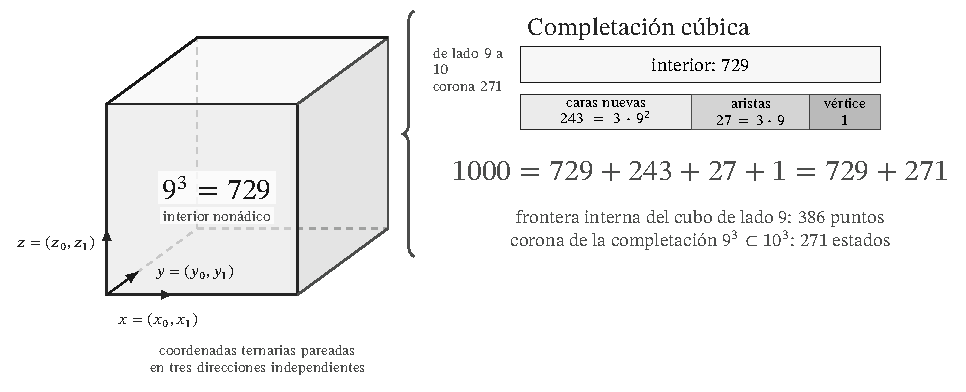
\includegraphics[width=\linewidth,keepaspectratio]{figures/cubo_emrh.pdf}
\caption{Representación cúbica de la ampliación de nueve a diez clases por coordenada. Los estratos \(S_1,S_2,S_3\) sitúan las incidencias añadidas en caras, aristas y ápice; sus cardinales forman la corona de \(271\) elementos. La frontera de \(386\) elementos pertenece al cubo inicial. La perspectiva geométrica complementa la partición de la figura~\ref{fig:revision-emrh}; las separaciones gráficas tienen función esquemática.}
\label{fig:completacion-cubo-recuperado}
\end{figure}

% END IX03_CUBIC_COMPLETION_FIGURE

\subsubsection{Conservación de la unidad y compatibilidad dimensional}

La normalización no se limita a dividir una identidad aislada. En dimensión
\(d\), el producto \(\widehat E^d\) lleva la medida uniforme
\(\mu_d(\{x\})=10^{-d}\). La proyección coordenada
\(p_d:\widehat E^{d+1}\to\widehat E^d\) suprime la última coordenada.

\begin{proposition}[Compatibilidad proyectiva de las medidas normalizadas]
Para todo \(d\geq1\),
\[
 (p_d)_*\mu_{d+1}=\mu_d,
 \qquad \mu_d(\widehat E^d)=1.
\]
La masa del estrato con \(r\) coordenadas adicionales es
\(\binom dr9^{d-r}/10^d\), y la suma de las masas de todos los estratos
es uno.
\end{proposition}
\begin{proof}
Cada punto de \(\widehat E^d\) tiene diez preimágenes. Su masa total es
\(10\,10^{-(d+1)}=10^{-d}\). La igualdad para cualquier subconjunto
se obtiene sumando sobre sus puntos. La fórmula estratificada procede
del mismo recuento que \eqref{eq:revision-estratos}; el binomio
\((9+1)^d\) da la normalización total.
\end{proof}

En dimensión tres, retirar el ápice deja masa \(999/1000\), y
restituirlo añade \(1/1000\). Renormalizar antes de la restitución
definiría otra medida: la distinción es operacionalmente relevante.
En particular, conservación de masa probabilística, conservación de los
registros de transporte y disipación termodinámica son afirmaciones con
objetos diferentes. La proposición demuestra la primera y proporciona el
soporte compatible para estudiar la segunda; la tercera requiere una
realización dinámica y energética especificada.

También permanece diferenciada la frontera geométrica interna.
Sobre el representante cartesiano \(\{1,\ldots,9\}^3\), retirar
\(\{2,\ldots,8\}^3\) deja \(386\) puntos. Esta frontera pertenece al
cubo inicial, mientras \(\widehat C\setminus C\) pertenece a su
ampliación. La completación cúbica, la expansión posicional de base mil y
la lectura de incidencia excepcional comparten datos del soporte;
sus mapas respectivos determinan qué información de esos datos utiliza
cada representación.


% Fragmento conservado; véase MANIFIESTO_ANTECEDENTES_LECTURA.json.
% Incorporación al final de extension.tex; no contiene una sección principal.
% Procedencia: RESULTADO_RECUPERADO; explicitación sectorial de las hipótesis.
% Fuentes leídas: monografía Doble proyección holográfica (cantera editorial),
% manuscrito/local/01_tesis_recuperada.tex y
% manuscrito/generated/algebra_holonomica.tex, especialmente §§1--7 y 21.
% Definición rectora de número: manuscrito/flattened/main_autosuficiente.tex,
% secciones que comienzan en líneas 22137 y 23000 de la cantera de 775 páginas.
% No se adopta su presentación global como prueba de todas las flechas TPK.

\subsection{El número como sección compatible y el valor como lectura}
\label{hist:seccion}

La distinción entre estado y observación permite precisar qué objeto se
prolonga cuando aumenta la resolución. A profundidad \(n\), sea \(X_n\)
el conjunto de estados admisibles producidos por APP--TRIT--TPK. Sus datos
incluyen posición, hojas suma y producto, residuos y cocientes, régimen,
orientación, acarreo, fase, ruta, frontera, memoria y supervivencia. No son
coordenadas independientes: las evaluaciones aritméticas y los transportes
anteriores imponen sus relaciones. Una prolongación conserva esas relaciones
en cada antecedente, aunque añada nuevos pasos y nuevos datos de memoria.
Éste es el sentido de la aritmética de historias desarrollada en
\textup{(procedencia conservada en el registro técnico)}.

Sean \(r_{m,n}:X_m\to X_n\), para \(m\geq n\), las restricciones de
profundidad, con \(r_{n,n}=\operatorname{id}\) y
\(r_{\ell,n}=r_{m,n}\circ r_{\ell,m}\). Cada restricción conserva el
prefijo y la información ya determinada en él.

\begin{definition}[Sección numérica compatible]
Un número HMT es una historia compatible del sistema de estados:
\begin{equation}
 x=(x_n)_{n\geq0}\in X_\infty:=\varprojlim_n X_n,
 \qquad r_{m,n}(x_m)=x_n.
 \label{hist:limite-inverso}
\end{equation}
Un lector es una operación adicional sobre un dominio especificado de estas
historias. Una cifra es una observación finita; un valor escalar es una
evaluación del lector. El par formado por la sección y su lector constituye
una presentación leída, no una redefinición de la identidad de la sección.
\end{definition}

En el dominio arquimediano \(X_\infty^{\mathrm{Arch}}\), el lector asocia
a cada prefijo un cilindro cerrado, conserva su encajamiento y hace tender
su diámetro a cero. Así determina
\begin{equation}
 \operatorname{ev}_{\mathbb R}:X_\infty^{\mathrm{Arch}}\longrightarrow
 \mathbb R,\qquad
 \{\operatorname{ev}_{\mathbb R}(x)\}=\bigcap_n I_n(x).
 \label{hist:evaluacion}
\end{equation}
La construcción concreta de estos cilindros y la decisión de sus fronteras
se desarrollan en la sección~\ref{sec:generacion}. La definición
\eqref{hist:limite-inverso} no afirma por sí sola que la imagen de
\eqref{hist:evaluacion} sea toda la recta: una afirmación de cobertura
requiere su propio teorema. Tampoco una igualdad de valores establece, sin
un resultado de inyectividad, la igualdad de sus historias. Esta separación
permite hablar de precisión como profundidad conservando la diferencia
entre el antecedente aritmético y su realización escalar.

\subsection{Composición de historias y multiplicador de memoria}
\label{hist:algebra}

Fijemos un sector de estados a profundidad \(n\) y una categoría
\(\mathcal C\) cuyas flechas sean sus historias admisibles. La composición
se escribe \(vu=v\circ u\): primero se recorre \(u\) y después \(v\).
Los pasos elementales proceden de la selección, el transporte y la
actualización del TPK. Una fibra trítica local admite la escritura
\(\mathbb R[J_x]/(J_x^2+\tau(x)1_x)\), donde
\(\tau(x)\in\{+1,0,-1\}\). El régimen y la orientación pertenecen al
estado que se transporta; una transición entre regímenes no equivale a
identificar sus álgebras cuadráticas.

La siguiente formulación precisa un sector algebraico de esa composición.
Para cada objeto \(x\), se da un álgebra real asociativa unitaria \(A_x\),
que puede ser no conmutativa. Para cada \(u:x\to y\), se da un
homomorfismo unital \(\rho_u:A_x\to A_y\). Suponemos una acción estricta:
\begin{equation}
 \rho_{\operatorname{id}_x}=\operatorname{id}_{A_x},\qquad
 \rho_v\rho_u=\rho_{vu}.
 \label{hist:accion-estricta}
\end{equation}
Para cada pareja componible \(u:x\to y\), \(v:y\to z\), fijamos un
multiplicador central invertible
\(\Omega(v,u)\in Z(A_z)^\times\). Se exige la normalización
\(\Omega(\operatorname{id}_y,u)=\Omega(u,\operatorname{id}_x)=1_y\)
y, para cada triple componible, la identidad
\begin{equation}
 \rho_w\bigl(\Omega(v,u)\bigr)\Omega(w,vu)
   =\Omega(w,v)\Omega(wv,u).
 \label{hist:cociclo}
\end{equation}
Son hipótesis explícitas sobre los transportes y sus coeficientes, no una
consecuencia de llamar holonómica a la dinámica. Al aplicar esta presentación
a un sector TPK deben identificarse sus \(\rho_u\) y \(\Omega(v,u)\).
Las transiciones expresadas mediante bimódulos requieren conservar esa
estructura y no quedan reemplazadas por \eqref{hist:accion-estricta}.

El espacio de sumas finitas
\[
 \mathcal H(\mathcal C,A,\rho,\Omega)
   =\bigoplus_{u\in\operatorname{Mor}(\mathcal C)} A_{t(u)}T_u
\]
recibe el producto bilineal
\begin{equation}
 (aT_v)(bT_u)=a\rho_v(b)\Omega(v,u)T_{vu},
 \label{hist:producto}
\end{equation}
si las flechas son componibles, y cero en otro caso. Aquí \(t(u)\)
designa el estado terminal. La suma reúne historias con coeficientes; el
producto concatena historias conservando el multiplicador del registro.

\begin{proposition}[Asociatividad sectorial con multiplicador central]
Bajo \eqref{hist:accion-estricta} y \eqref{hist:cociclo}, el producto
\eqref{hist:producto} es asociativo. Si el conjunto de objetos es finito,
su unidad es \(\sum_x1_xT_{\operatorname{id}_x}\).
\end{proposition}
\begin{proof}
Para \(u:x\to y\), \(v:y\to z\), \(w:z\to t\), sean
\(a\in A_y\), \(b\in A_z\), \(c\in A_t\). Los dos coeficientes
de \(T_{wvu}\) son
\begin{align*}
 ((cT_w)(bT_v))(aT_u):\quad&
 c\rho_w(b)\Omega(w,v)\rho_{wv}(a)\Omega(wv,u),\\
 (cT_w)((bT_v)(aT_u)):\quad&
 c\rho_w(b)\rho_w\rho_v(a)\rho_w(\Omega(v,u))\Omega(w,vu).
\end{align*}
La acción estricta iguala \(\rho_w\rho_v(a)\) con \(\rho_{wv}(a)\).
La centralidad de \(\Omega(w,v)\) permite desplazarlo a la derecha de
ese factor; \eqref{hist:cociclo} iguala entonces los productos restantes.
No se permutan los coeficientes \(a,b,c\). Si el triple no es componible,
ambas parentizaciones son cero por sus estados iniciales y terminales.
La bilinealidad concluye la prueba. Las identidades locales y la
normalización de \(\Omega\) verifican la unidad indicada.
\end{proof}

El acarreo del calendario proporciona un ejemplo efectivo. En la categoría
de un objeto y flechas \(C_9\), tomemos coeficientes
\(A=\mathbb R[z,z^{-1}]\), acción identidad y
\[
 \Omega(b,a)=z^{c_0(a,b)},\qquad
 c_0(a,b)=\left\lfloor\frac{a+b}{9}\right\rfloor,
 \quad 0\leq a,b<9.
\]
Las dos sumas de acarreos de un triple son
\(\lfloor(a+b+c)/9\rfloor\); por ello se cumple
\eqref{hist:cociclo}. La variable formal \(z\) registra la vuelta sin
asignarle un valor numérico. Imponer después \(z^{12}=1\) recupera el
registro dodecafásico del calendario \eqref{eq:extension108}; conservar
\(z\) sin esa relación distingue vueltas sucesivas. El ejemplo realiza
la memoria de este calendario, sin identificarla con la totalidad de la
memoria TPK.

\subsection{Doble varianza del refinamiento y conservación de la unidad}
\label{hist:doble-varianza}

Al restringir estados se prolongan observables en sentido contrario.
Consideremos las álgebras de funciones, con producto puntual,
\(D_n=\operatorname{Fun}(X_n,\mathbb R)\). La precomposición define
\begin{equation}
 r_{m,n}^*:D_n\longrightarrow D_m,
 \qquad r_{m,n}^*f=f\circ r_{m,n}.
 \label{hist:precomposicion}
\end{equation}
Son morfismos unitales; son además inyectivos cuando las restricciones
correspondientes son sobreyectivas. El límite directo
\(D_{\mathrm{cyl}}=\varinjlim_n(D_n,r_{n+1,n}^*)\) reúne las
observaciones de profundidad finita. No se identifica aquí este álgebra
con toda el álgebra de rutas: prolongar los operadores de transporte exige
también sus compatibilidades con el refinamiento.

\begin{lemma}[Unidad y naturalidad de la evaluación]
Si \(e_x\) es el indicador de \(x\in X_n\), se cumple
\begin{equation}
 r_{m,n}^*e_x=\sum_{y:\,r_{m,n}(y)=x}e_y,
 \qquad r_{m,n}^*1_n=1_m,
 \label{hist:unidad}
\end{equation}
y, para todo \(f\in D_n\), \(y\in X_m\),
\[
 \langle r_{m,n}^*f,y\rangle=\langle f,r_{m,n}y\rangle.
\]
Cada sección \(x\in X_\infty\) determina una evaluación bien definida
\(D_{\mathrm{cyl}}\to\mathbb R\), dada por \([f]\mapsto f(x_n)\)
para \(f\in D_n\).
\end{lemma}
\begin{proof}
Las fibras de \(r_{m,n}\) forman una partición de \(X_m\). Sus
indicadores son ortogonales y suman \(1_m\), lo que prueba
\eqref{hist:unidad}. La naturalidad es la definición de precomposición.
Finalmente, \((r_{m,n}^*f)(x_m)=f(x_n)\), de modo que dos representantes
compatibles dan la misma evaluación en el límite directo.
\end{proof}

La unidad global es la función constante uno sobre todas las posibilidades;
la sección individual selecciona una historia compatible. Conservar la
primera no significa inmovilizar la segunda. El refinamiento puede aumentar
la cantidad de extensiones y la profundidad de cada historia manteniendo
la unidad y todas las evaluaciones de sus antecedentes.



\clearpage
% Fragmento conservado; véase MANIFIESTO_ANTECEDENTES_LECTURA.json.
\section{Generación coinductiva de \texorpdfstring{\(\pi,\varphi,e\)}{pi, phi, e} a profundidad arbitraria}
\label{sec:generacion}

La emisión de seis bloques es una etapa finita de la construcción, no una expansión decimal completa. Su función consiste en producir regiones con multiplicidad, orientación y reglas de transporte. La prolongación debe conservar esos datos y determinar una colección compatible de prefijos de longitud arbitraria. La palabra \emph{generación} designa esta operación; \emph{genealogía} designa la reconstrucción de sus dependencias. Ambas nociones intervienen, pero cumplen funciones distintas.

\subsection{Órbitas, regiones y caracteres de clausura, propagación y autoescala}

Sobre una palabra \(w=(w_1,\ldots,w_6)\), definimos
\[
 r(w)=(w_3,w_1,w_2,w_5,w_6,w_4),\qquad
 s(w)=(w_4,w_5,w_6,w_1,w_2,w_3).
\]
Se cumple \(r^3=s^2=I\) y \(srs=r^{-1}\); por tanto estas permutaciones realizan el grupo diedral \(D_3\). La acción conserva el catálogo y las multiplicidades y conmuta con \(\Psi\). El cociente de las \(243\) palabras visibles tiene \(43\) órbitas: treinta y ocho de cardinal seis y cinco de cardinal tres.

La clase de clausura se reconoce por un predicado de fibra: sus seis orientaciones tienen cinco emisiones por palabra, multiplicidad total \(1008\) y distribución \(432+4\cdot144\). Existe una sola órbita con esas propiedades en el catálogo. Para precisar las otras dos selecciones, escribimos \(f(w)=\#\Psi^{-1}(w)\), \(m(w)=\sum_{U\in\Psi^{-1}(w)}\operatorname{mult}(U)\) y \(\nu(w)=(n_0,n_1,n_2)\). La clase diagonal aditiva de una emisión es \(d(U)=[i+j]_9\) en los índices de cero a ocho; su firma aditiva conserva esta clase y la orientación \(ES\) o \(NO\). Sea \(\mathcal D(\mathcal O)\) el conjunto de esas clases para todas las emisiones sobre una órbita.

Entre las órbitas de tamaño seis, el predicado conjunto
\[
 f(w)=1,\qquad m(w)=144\quad(w\in\mathcal O),\qquad
 \mathcal D(\mathcal O)=\{0,3,6\}
\]
deja exactamente seis órbitas. En este sector, el censo \(\nu=(2,3,1)\), igual al de clausura, selecciona únicamente la propagación; el censo \(\nu=(2,2,2)\) selecciona únicamente la autoescala. El soporte diagonal no puede omitirse: sin él hay cuatro órbitas unipuntuales equilibradas de multiplicidad \(144\), no una. Finalmente, la existencia de una emisión con \(d=6\) y orientación \(ES\) selecciona un representante de cada órbita y conduce a
\begin{equation}
 w^{\rm cl}=010211,\qquad w^{\rm pr}=201101,\qquad w^{\rm au}=121200.
 \label{eq:palabras-regionales}
\end{equation}
Estos símbolos designan primero regiones del catálogo. La identificación escalar se demostrará mediante sus lectores; no se eligen porque coincidan con cifras de una constante conocida.

La palabra de clausura \(010211\) tiene las cinco preimágenes siguientes:
\begin{center}\small
\begin{tabular}{@{}lll r@{}}\toprule
Emisión de seis bloques&Firma multiplicativa&Papel&Multiplicidad\\\midrule
\(501,614,498,169,272,272\)&\(555555\)&transversal&432\\
\(810,923,870,169,272,272\)&\(339555\)&orientación positiva&144\\
\(810,983,810,169,272,272\)&\(393555\)&orientación positiva&144\\
\(870,923,810,169,272,272\)&\(933555\)&orientación positiva&144\\
\(870,923,810,418,674,521\)&\(933717\)&retorno orientado&144\\\bottomrule
\end{tabular}
\end{center}
La multiplicidad \(432\) y la firma constante \(555555\) caracterizan la región transversal. No identifican la posición central \((5,5)\) de APP. Confundir una firma de seis ventanas con una posición del soporte eliminaría la distinción entre región numérica y estructura electrónica.

La microfibra posee además una morfología bipartita precisa. Cada emisión es un producto de una clase de cursor aditivo y una clase multiplicativa. Las tres regiones positivas comparten la misma clase aditiva de dieciocho condiciones; juntas contienen tres clases multiplicativas de ocho condiciones cada una. La región transversal posee un producto \(18\times24\); las tres positivas reunidas, otro \(18\times24\); y el retorno, un producto \(18\times8\). La descomposición por emisiones tiene cinco partes, mientras la descomposición por componentes conexas del grafo bipartito tiene tres. Ambas conservan las mismas \(1008\) semillas sin reducir la forma a un cardinal.

\subsection{Transporte finito y frontera de prolongación}

Los endomorfismos \(L_0,L_1\) del espacio de palabras ternarias actúan antes de la realización arquimediana. Su determinación comienza por las transiciones del estado aritmético, no por la prescripción de dos matrices. Si \(U_t\) es el paso compuesto de selección, transporte y actualización, el bloque observado satisface
\[
 b_j^\chi=\Pi_6(x_j^\chi),\qquad
 x_{j+1}^\chi=U_{9j+9}\cdots U_{9j+1}(x_j^\chi),
 \qquad \chi\in\{\mathrm{cl},\mathrm{pr},\mathrm{au}\}.
\]
Se forman seis transiciones por cada régimen: dos consecutivas en cada una de las tres regiones. Los pares de matrices de orígenes y destinos obtenidos en el registro son
\[
\begin{array}{c|c|c|c}
X_0&Y_0&X_1&Y_1\\\hline
010211&012222&010211&002111\\
012222&010211&002111&110221\\
201101&121221&102011&012222\\
121221&102011&012222&102011\\
121200&112202&121020&010210\\
112202&121020&010210&010200
\end{array}
\]
Cada cadena de seis dígitos representa una fila en \(\FF_3^6\). Puesto que \(\det X_0=1\) y \(\det X_1=-1\) en \(\FF_3\), las ecuaciones \(X_aL_a=Y_a\) determinan unívocamente \(L_a=X_a^{-1}Y_a\). En esa coordenatización de vectores fila resultan
\[
 L_0=\begin{pmatrix}
 2&2&2&1&2&1\\2&1&2&2&1&1\\1&0&0&1&0&2\\
 0&0&1&1&1&0\\2&2&2&0&2&1\\2&1&2&1&0&0
 \end{pmatrix},\quad
 L_1=\begin{pmatrix}
 2&1&2&0&2&2\\1&2&1&1&2&0\\1&2&1&1&1&2\\
 0&1&0&0&2&1\\2&0&2&1&0&1\\0&2&2&2&1&1
 \end{pmatrix}\quad(\bmod3).
\]
El calendario \((L_0,L_0,L_1,L_1)\) produce cuatro nuevos bloques de seis componentes. Sus concatenaciones forman
\[
 w_6\longrightarrow w_{12}\longrightarrow w_{18}
 \longrightarrow w_{24}\longrightarrow w_{30}.
\]
Los subíndices de \(w\) indican longitud acumulada. La frontera \(R_{36}\) conserva la estructura terminal y abre la relación de prolongación; no se renombra como un último bloque periódico que pudiera repetirse indefinidamente.

La identidad \(L=X^{-1}Y\) demuestra unicidad una vez fijadas las transiciones; no sustituye la producción de esas transiciones por \(U_t\). La procedencia de su registro y el examen de los dieciséis calendarios binarios se documentan en el suplemento técnico. El calendario indicado es el único de esos dieciséis que reproduce conjuntamente las tres sucesiones de cinco bloques.

\subsection{Cinco regiones de clausura y compensación angular}

La región de clausura contiene una componente transversal y cuatro acompañantes. El lector simétrico actúa en el espacio de sus cinco posiciones mediante
\[
 P_5=\frac15\mathbf1\mathbf1^{\mathsf T},\qquad
 \mathbf1=(1,1,1,1,1)^{\mathsf T}.
\]
La invariancia \(P_5\lambda=\lambda\) y la conservación \(\mathbf1^{\mathsf T}\lambda=1\) fuerzan \(\lambda=\mathbf1/5\). Esta normalización distribuye la unidad entre posiciones del lector; no sustituye las multiplicidades de semillas \(432,144,144,144,144\) por frecuencias uniformes. La coordenatización elíptica del lector realiza cada coordenada mediante \(1+\lambda_jJ\); su pendiente es \(\lambda_j\), por lo que la pendiente primitiva resulta \(1/5\). Se hace explícita así la regla que pasa de una coordenada normalizada a una pendiente, en lugar de identificar ambas nociones sin mapa. El lector compone las cuatro posiciones acompañantes por la ley
\begin{equation}
 a\oplus b=\frac{a+b}{1-ab}.
 \label{eq:suma-pendientes}
\end{equation}
Esta ley se obtiene al multiplicar \((1+aJ)(1+bJ)\) en el régimen \(J^2=-I\) y dividir por su componente escalar. Por ello la composición de pendientes es una realización de la estructura cuadrática de TRIT, no una suma ordinaria de cuatro fracciones.

\begin{proposition}[Compensador de la clausura]
La composición de cuatro pendientes \(1/5\) es \(120/119\). La condición de retorno a pendiente uno determina un único compensador positivo de la forma \(1/q\), con \(q>1\), y da \(q=239\).
\end{proposition}
\begin{proof}
La primera duplicación da \((1/5)\oplus(1/5)=5/12\); la segunda, \((5/12)\oplus(5/12)=120/119\). La condición
\[
 \frac{120/119-1/q}{1+(120/119)/q}=1
\]
equivale a \((120-119)q=120+119\), por lo que \(q=239\).
\end{proof}

El carácter de clausura resultante tiene realización
\begin{equation}
 \Pi_{\rm cl}=4\left(4\arctan\frac15-\arctan\frac1{239}\right).
 \label{eq:lector-pi}
\end{equation}
La identidad angular de Machin reconoce \(\Pi_{\rm cl}=\pi\). El sentido de la construcción es preciso: la pendiente y el número de composiciones están declarados por el lector de la pentafibra; la ecuación de compensación fuerza \(239\). Una vez producido este carácter, su evaluación por series alternadas no selecciona de nuevo la órbita de semillas.

Para \(0<x<1\), las sumas alternadas
\[
 A_n(x)=\sum_{j=0}^n\frac{(-1)^jx^{2j+1}}{2j+1}
\]
encierran \(\arctan x\) entre dos truncamientos consecutivos, con diferencia \(x^{2n+3}/(2n+3)\). Aplicadas a las dos pendientes de \eqref{eq:lector-pi}, proporcionan extremos racionales de error explícito. El valor numérico se calcula así como consecuencia del carácter exacto, sin introducir un prefijo objetivo.

\subsection{Lector de propagación y normalización de la unidad}

La región de propagación se realiza mediante una colección formal \(P_t\in\mathcal A[[t]]\), donde \(\mathcal A\) es un álgebra conmutativa unitaria sobre \(\QQ\). Su composición satisface \(P_{t+s}=P_tP_s\), con unidad \(P_0=1\), y el transporte elemental orientado fija el generador escalar \(P'_0=+1\). La condición fija su signo, no sólo su magnitud. Escribiendo
\[
 P_t=\sum_{n\ge0}a_nt^n,
\]
la normalización determina \(a_0=a_1=1\). La comparación del coeficiente de \(s^nt\) en \(P_{s+t}=P_sP_t\) da \((n+1)a_{n+1}=a_na_1\); equivalentemente, \(P'_t=P_t\). Así,
\begin{equation}
 (n+1)a_{n+1}=a_n,\qquad a_n=\frac1{n!}.
 \label{eq:propagacion}
\end{equation}
El carácter en una unidad de parámetro es \(\Pi_{\rm pr}=P_1\), reconocido posteriormente como \(e\).

La normalización del generador importa. La ley semigrupal sin ese dato admitiría \(P_t=e^{ct}\) para distintos \(c\); por ello no se omite la condición que fija la unidad del parámetro en el lector. Esta condición es anterior a la comparación decimal y pertenece a la exposición de la regla operacional, no a la elección de un valor experimental.

\begin{proposition}[Cotas racionales de propagación]
Para \(n\ge1\), sea \(E_n=\sum_{j=0}^n1/j!\). Entonces
\[
 E_n<\Pi_{\rm pr}<E_n+\frac{n+2}{(n+1)(n+1)!}.
\]
\end{proposition}
\begin{proof}
El primer término omitido es \(1/(n+1)!\). Cada cociente posterior es a lo sumo \(1/(n+2)\). La suma geométrica mayorante de la cola es
\[
 \frac1{(n+1)!}\frac1{1-1/(n+2)}
 =\frac{n+2}{(n+1)(n+1)!}.
\]
La desigualdad estricta se sigue de la disminución de los cocientes sucesivos.
\end{proof}

\subsection{Incidencia modal y generación de la autoescala}

El selector trítico produce el ciclo \((+1,-1,0)\). En los modos \(\Sigma,\Pi\), la regla es \(+1:m\mapsto\Sigma\), \(-1:m\mapsto\Pi\), \(0:m\mapsto m\). Con cierre cíclico, el modo observado es \((\Sigma,\Pi,\Pi)\). Sus aristas son \(\Sigma\to\Pi\), \(\Pi\to\Pi\) y \(\Pi\to\Sigma\). Por tanto su incidencia, en ese orden de modos, es
\begin{equation}
 F_{\rm av}=\begin{pmatrix}0&1\\1&1\end{pmatrix}.
 \label{eq:fav}
\end{equation}
Las cuatro entradas se obtienen del calendario, no de una ecuación que haya recibido previamente el valor de \(\varphi\). La repetición del calendario da conteos \(3F_{\rm av},9F_{\rm av},36F_{\rm av}\) en longitudes nueve, veintisiete y ciento ocho. Estos conteos no son las potencias de la matriz.

\begin{theorem}[Carácter positivo de autoescala]
La incidencia \eqref{eq:fav} posee un único rayo propio estrictamente positivo. Al normalizarlo como \((1,x)^{\mathsf T}\), su coordenada \(x\) satisface \(x^2-x-1=0\), \(x>0\), y es \(\varphi=(1+\sqrt5)/2\).
\end{theorem}
\begin{proof}
La ecuación propia da \(x=\lambda\) y \(1+x=\lambda x\). Eliminar \(\lambda\) produce el polinomio. De sus dos raíces sólo una es positiva. Como \(F_{\rm av}^2\) tiene todas sus entradas positivas, el rayo positivo es único y simple. La expresión radical reconoce la coordenada obtenida; no participa en la producción de \(F_{\rm av}\).
\end{proof}

Con \(F_0=0,F_1=1,F_{n+1}=F_n+F_{n-1}\), la incidencia induce, para \(n\geq1\),
\[
 F_{\rm av}^n=\begin{pmatrix}F_{n-1}&F_n\\F_n&F_{n+1}\end{pmatrix}.
\]
Los cocientes consecutivos \(F_{n+1}/F_n\) alternan alrededor de \(\varphi\). La identidad de determinante
\[
 F_{n+1}^2-F_nF_{n+2}=(-1)^n
\]
da una anchura exacta \(1/(F_nF_{n+1})\) entre dos cocientes consecutivos. Su crecimiento hace arbitrariamente pequeña esta horquilla racional.

\subsection{Cilindros compatibles y profundidad arbitraria}

La realización de un bloque ternario \(b=(b_1,\ldots,b_6)\) es el entero
\[
 \nu(b)=\sum_{j=1}^6b_j3^{6-j}\in\{0,\ldots,728\}.
\]
Una sucesión de bloques define prefijos enteros por \(N_{n+1}=729N_n+\nu(b_{n+1})\), comenzando en \(N_0=m\), donde \(m\) es la parte entera determinada por el lector. Las horquillas anteriores sitúan los caracteres de clausura, propagación y autoescala en \((3,4)\), \((2,3)\) y \((1,2)\), respectivamente; por tanto, sus valores iniciales son \(m=3,2,1\). Los bloques siguientes refinan la parte fraccionaria. El cilindro correspondiente es
\begin{equation}
 I_n=\left[\frac{N_n}{729^n},\frac{N_n+1}{729^n}\right],
 \qquad |I_n|=729^{-n}.
 \label{eq:cilindro}
\end{equation}
La convención semiabierta se utiliza para seleccionar un representante cuando un valor cae en una frontera. Para el paso al límite se utilizan las clausuras de estos intervalos y se identifican las dos expansiones fronterizas equivalentes. Esta precisión impide suponer que toda intersección de intervalos semiabiertos encajados sea automáticamente no vacía.

\begin{theorem}[Determinación de la realización escalar]
Una historia de bloques compatible determina un único límite de los extremos izquierdos de \eqref{eq:cilindro}. Si un carácter exacto dispone de horquillas racionales de anchura arbitrariamente pequeña y se separa de la frontera de cada cilindro decimal examinado, cada prefijo decimal de longitud finita se determina después de un cálculo finito. Los prefijos así obtenidos son compatibles entre sí.
\end{theorem}
\begin{proof}
La extensión de un bloque conserva el prefijo anterior por división euclídea. Los cilindros cerrados están encajados y su diámetro tiende a cero; sus extremos izquierdos son de Cauchy y tienen un único límite. Para una longitud decimal fijada, un valor separado de las fronteras de la partición posee distancia positiva a ellas. Una horquilla suficientemente estrecha queda contenida en una única celda y determina su prefijo. La unicidad de la celda y el encajamiento de las particiones prueban la compatibilidad por truncamiento. En los puntos con expansión terminal debe añadirse la decisión exacta de frontera y su convención de representación; no se deduce esa decisión de una anchura numérica solamente.
\end{proof}

\begin{corollary}[Obtención finita y compatibilidad de los prefijos regionales]
\label{gen:prefijos-regionales}
Para cada una de las realizaciones \(\pi,\varphi,e\) y para toda longitud
decimal finita, las horquillas construidas determinan el prefijo correspondiente
mediante un cálculo finito. Los prefijos obtenidos a distintas profundidades
son compatibles por truncamiento.
\end{corollary}
\begin{proof}
Los caracteres de clausura, propagación y autoescala poseen las horquillas
anteriores. Tras su reconocimiento, la irracionalidad de \(\pi,e,\varphi\)
garantiza su separación de las fronteras racionales de cada partición decimal
finita. Se aplica el teorema precedente a cada carácter.
\end{proof}
La profundidad arbitraria expresa el cuantificador del corolario: para todo
horizonte finito existe un cálculo que determina su prefijo. El objeto
matemático es la colección compatible completa; cada ejecución obtiene una
proyección finita de ella.

\subsection{Involución especular y sincronización de las regiones}

La conexión nonádica transporta conjuntamente los tres caracteres. En la coordenatización de la novena fase, el eje de autoescala y la suma ternaria de clausura y propagación permanecen fijados bajo el intercambio especular. La inversión helicoidal cambia el sentido del transporte; el espejo de los dos canales cambia su orientación relativa. Son involuciones diferentes, aunque ambas actúen sobre el mismo sistema de trayectorias.

Las coincidencias de censo ilustran esa coordinación:
\begin{center}
\begin{tabular}{@{}c rrr l@{}}\toprule
Fase&\(N_\pi\)&\(N_e\)&\(N_\varphi\)&Igualdad de conteos\\\midrule
4&207&207&122&\(N_\pi=N_e\)\\
5&39&151&151&\(N_e=N_\varphi\)\\
6&110&110&69&\(N_\pi=N_e\)\\
7&81&29&81&\(N_\varphi=N_\pi\)\\
8&59&59&59&sincronización triple\\
9&43&43&43&sincronización triple\\\bottomrule
\end{tabular}
\end{center}
Estos enteros cuentan coordenadas compatibles de las regiones. No afirman una igualdad entre \(\pi\), \(e\) y \(\varphi\) como números reales. Si
\[
 \partial(a,b,c)=(a-b,b-c,c-a),
\]
su imagen pertenece al retículo \(A_2=\{(u,v,w)\in\ZZ^3:u+v+w=0\}\). En las fases ocho y nueve la componente relativa se anula, pero la componente diagonal cambia de \((59,59,59)\) a \((43,43,43)\). La sincronización relativa coexiste con un desplazamiento de \(-16\) por canal. El cierre que conducirá a \(\alpha\) debe conservar ambas informaciones: coincidencia relativa y evolución de la memoria.


% Fragmento conservado; véase MANIFIESTO_ANTECEDENTES_LECTURA.json.
\subsection{Simetría especular de las regiones y doble realización}
\label{mono-ampl:regiones}

El intercambio especular actúa en el bloque regional
\(B=(u^\pi,u^e,u^\varphi)\in(\mathbb F_3^6)^3\) por
\[
 \mathfrak cB=(u^e,u^\pi,u^\varphi).
\]
Su eje fijo y su agregado son, respectivamente, \(u^\varphi\) y
\(s=u^\pi+u^e\). Esta fijación se refiere a la involución en una fibra;
ambas coordenadas pueden evolucionar durante el transporte nonádico.
Con \(q=u^\pi+u^e+u^\varphi\),
\(a=u^\pi+u^e-u^\varphi\) y \(d=u^\pi-u^e\), se recupera
\[
 u^\varphi=2(q-a),\qquad s=q-u^\varphi,\qquad
 u^\pi=2(s+d),\qquad u^e=2(s-d).
\]
Las igualdades son componente a componente en \(\mathbb F_3\), donde
\(2^{-1}=2\). El espejo conserva \(q,a,s\) e invierte \(d\); esta
coordenada antisimétrica individualiza el reparto que el agregado conserva
sin distinguir. La inversión \(\mathcal I\) del índice temporal y la
involución \(\mathfrak c\) de canales actúan, por consiguiente, sobre
datos diferentes.

El retorno de fase posee un testigo explícito:
\[
 \begin{aligned}
 B_1&=(012222\mid121221\mid112202),\\
 B_{10}&=(101222\mid112221\mid112002).
 \end{aligned}
\]
Las dos posiciones tienen fase \(1\); el bloque, el eje y la memoria han
cambiado. Asimismo, la sincronización de los censos en las fases \(8\) y
\(9\) anula sus diferencias relativas, mientras la componente diagonal
pasa de \((59,59,59)\) a \((43,43,43)\). La igualdad de un observable
relativo no agota el estado que lo determina.

La doble realización conserva esa arquitectura. En la sección
8.1 del Artículo I (procedencia del corredor excepcional, conservada en el registro técnico), el mismo prefijo determina por una parte cilindros
encajados y por otra una sucesión de palabras codificadas con sus marcos.
El primer mapa pasa al límite por contracción de diámetros; el segundo
satisface \(r_{n,m}Q_n=Q_mp_{n,m}\) y define \(Q_\infty\).
La figura \ref{mono-ampl:fig-regional} anticipa esas dos aplicaciones.
El recorrido incidencial posterior construye códigos, retículos y la
realización de Moonshine en sus dominios propios; el grupo de automorfismos
actúa sobre esa realización, no sobre las cifras por una identificación
implícita.

% Fragmento conservado; véase MANIFIESTO_ANTECEDENTES_LECTURA.json.
% Figura acumulativa; destino figures/monodromia_regional_ampliacion.tex.
\begin{figure}[!htbp]
\centering
\begin{tikzpicture}[x=1cm,y=1cm,>=Latex,font=\small,
  flow/.style={->,line width=.55pt},
  ann/.style={align=center,font=\footnotesize}]
\node[font=\bfseries] at (6.9,9.2)
  {Conexión nonádica y coordenadas regionales};
\begin{scope}[shift={(3.4,6.8)}]
 \foreach \k in {1,...,9}{
  \pgfmathsetmacro{\ang}{90-40*(\k-1)}
  \coordinate (p\k) at (\ang:1.52);
  \fill (p\k) circle (1.4pt);
  \node[fill=white,inner sep=1.1pt,font=\footnotesize]
    at (\ang:1.83) {\(\k\)};
 }
 \foreach \k in {1,...,8}{
  \pgfmathtruncatemacro{\next}{\k+1}
  \draw[flow,shorten >=3pt,shorten <=3pt] (p\k)--(p\next);
 }
 \draw[flow,shorten >=3pt,shorten <=3pt] (p9)--(p1);
 \node[ann] at (0,.1) {\(g_k\in C_9\)\\\(\Gamma_{9,k}\)};
 \node[ann] at (0,-2.23) {Una vuelta: \(g\mapsto g\), \(m\mapsto m+1\)};
\end{scope}
\node[ann,text width=5.25cm] at (10.1,7.75)
 {\(B_k=(u_k^\pi,u_k^e,u_k^\varphi)\)\\
 bloque regional en una fibra};
\node at (8.55,6.5) {\(u^\pi\)};
\node at (11.65,6.5) {\(u^e\)};
\draw[<->,line width=.65pt] (8.95,6.5)--node[above]{\(\mathfrak c\)}(11.25,6.5);
\draw[densely dashed,gray] (10.1,5.72)--(10.1,7.23);
\node[fill=white,inner sep=2pt] at (10.1,5.6){\(u^\varphi\)};
\node[ann] at (10.1,4.6)
 {Eje \(u^\varphi\) y agregado \(u^\pi+u^e\)\\
 invariantes bajo \(\mathfrak c\)};
\draw[flow] (5.45,6.8)--(7.25,6.8);
\draw[gray!60,line width=.3pt] (.55,4.02)--(13.25,4.02);
\node[ann,text width=12cm] (hist) at (6.9,3.47)
 {Historia compatible: prefijos, cilindros, orientación, cocientes,
 marcos de incidencia y memoria};
\coordinate (fork) at (6.9,2.85);
\draw[flow] (hist.south)--(fork);
\draw[flow] (fork)--(3.6,2.2);
\draw[flow] (fork)--(10.3,2.2);
\node[ann,text width=5.6cm] at (3.6,1.65)
 {Realización arquimediana\\
 \(I_{n+1}\subseteq I_n,\quad |I_n|=729^{-n}\)\\
 límite de los prefijos regionales};
\node[ann,text width=5.6cm] at (10.3,1.65)
 {Realización incidencial\\
 \(r_{n,m}Q_n=Q_mp_{n,m}\)\\
 palabras codificadas y marcos compatibles};
\node[ann,text width=5.6cm] at (3.6,.42)
 {\(\pi,\varphi,e\); determinación dodecafásica de \(\alpha\)};
\node[ann,text width=5.6cm] at (10.3,.42)
 {Witt--Golay--Leech--\(V^\natural\)\\
 automorfismos de la realización excepcional};
\draw[flow] (3.6,1.03)--(3.6,.78);
\draw[flow] (10.3,1.03)--(10.3,.78);
\end{tikzpicture}
\caption{\fontsize{9}{11}\selectfont Nueve fases de una conexión y dos realizaciones de la historia
compatible. El ciclo representa la fase; cada vuelta incrementa el contador.
El diagrama regional representa la involución \(\mathfrak c\), que
intercambia clausura y propagación y fija el eje de autoescala en una fibra.
Esta invariancia no impone que el eje sea constante durante el transporte.
Las dos aplicaciones inferiores utilizan el mismo prefijo: una determina
su límite numérico y la otra conserva palabras y marcos de incidencia. Los
mapas de esta segunda realización se especifican en la sección
8.1 del Artículo I (procedencia del corredor excepcional, conservada en el registro técnico); el recorrido excepcional se desarrolla después.}
\label{mono-ampl:fig-regional}
\end{figure}



\clearpage
% BEGIN NUCLEO_ADITIVO_20260921_SELECCION
\clearpage
% Ampliación demostrativa DF003--DF007. No modifica la fuente integral.
% Propietario común de los archivos Lean citados en estos comentarios:
% output/PAQUETE_ARTICULO_I_INTEGRACION_ESTADO_CAMPOS_20260919/.
% Residencia causal de la primera sección: después de los lectores regionales
% coinductivos y antes de emplear sus registros como entrada de la selección K.
% Residencia causal de la segunda sección: después de la construcción marcada
% Paley--Witt--Golay--Leech y antes de la reconstrucción de la estructura VOA.
% Los dos cortes expositivos conservan el mismo origen APP--TRIT--TPK.

\section[Generación regional y refinamiento]{Compatibilidad integral de la generación regional, el refinamiento cilíndrico y la incidencia}
\label{act21:sec:df-lectores-cilindros}

La prolongación regional produce sucesiones ordenadas de bloques, junto con
sus profundidades de lectura. La proyección arquimediana y la incidencia
ternaria se calculan sobre esas mismas sucesiones. El vínculo entre ambas
realizaciones puede formularse enteramente mediante operaciones enteras:
selección por intervalos racionales, división euclídea, elevación de seis
trits, lectura de acarreo y transformación de Witt. Esta formulación permite
seguir cada coeficiente desde su bloque generador hasta su empleo posterior.

La construcción utiliza los tres lectores regionales ya obtenidos del estado
APP--TRIT--TPK. Los denotaremos por los índices
\(c\in\{\mathrm P,\mathrm E,\mathrm F\}\), correspondientes, respectivamente,
a las regiones de clausura, propagación y autoescala. Su realización real se
escribirá \(v_c\). Las identificaciones posteriores
\(v_{\mathrm P}=\pi_{\mathrm{HMT}}\),
\(v_{\mathrm E}=e_{\mathrm{HMT}}\) y
\(v_{\mathrm F}=\varphi_{\mathrm{HMT}}\) conservan ese orden causal.
La operación que emite un bloque inspecciona los intervalos racionales del
lector regional; el valor real interviene en la demostración de corrección
de dicha operación.

\subsection{Emisión posicional mediante separación racional de celdas}
\label{act21:subsec:df-emision-racional}

% Fuente: lean/biblioteca/RegionalPublicationComposition.lean,
% produced_brackets, eventual_publication, joint_eventual_publication,
% search_terminates, stopped_cell_correct, publications_compatible.

Para cada región se dispone de dos sucesiones racionales
\(\ell_c(j),u_c(j)\), construidas por su lector, que cumplen
\[
 \ell_c(j)\leq v_c\leq u_c(j).
\]
La propiedad de separación de celdas demostrada para esos lectores afirma
que, para cada entero \(s>0\), existe \(J\) tal que, para todo \(j\geq J\),
\begin{equation}
 \lfloor s\ell_c(j)\rfloor
 =\lceil su_c(j)\rceil-1
 =\lfloor sv_c\rfloor.
 \label{act21:eq:df-separacion-celdas}
\end{equation}
La evitación de las fronteras racionales por los valores regionales es la
hipótesis de los teoremas previos que garantiza esta separación. Aquí se
emplea su conclusión operativa, con los lectores y los intervalos que la
producen.

\begin{definition}[Índice de separación y prefijo emitido]
Para \(s>0\), sea
\[
 j_c(s)=\min\{j\in\mathbb N:
 \lfloor s\ell_c(j)\rfloor=\lceil su_c(j)\rceil-1\}.
\]
Para una base entera \(b\geq2\) y una profundidad \(n\geq0\), se define
\begin{equation}
 P_c(b,n)=\lfloor b^n\ell_c(j_c(b^n))\rfloor.
 \label{act21:eq:df-publicacion-prefijo}
\end{equation}
El prefijo contiene la parte entera y las primeras \(n\) posiciones en base
\(b\); por consiguiente, \(P_c(b,0)\) es la parte entera regional.
\end{definition}

\begin{theorem}[Terminación y corrección de la emisión]
\label{act21:thm:df-emision-correcta}
El índice \(j_c(s)\) existe para todo \(s>0\). Los prefijos emitidos cumplen
\begin{equation}
 P_c(b,n)=\lfloor b^n v_c\rfloor,
 \qquad
 P_c(b,n)\leq b^n v_c<P_c(b,n)+1.
 \label{act21:eq:df-prefijo-correcto}
\end{equation}
Para cada escala \(s\) puede elegirse además un único índice de suficiencia
\(J(s)\) válido simultáneamente para las tres regiones.
\end{theorem}

\begin{proof}
La igualdad eventual de \eqref{act21:eq:df-separacion-celdas} hace no vacío el
conjunto que define \(j_c(s)\). Su mínimo existe por buen orden de
\(\mathbb N\). En cualquier índice donde se produzca la igualdad, la cota
inferior racional proporciona
\(\lfloor s\ell_c(j)\rfloor\leq\lfloor sv_c\rfloor\).
La cota superior, junto con la evitación de una frontera de celda, da
\(\lfloor sv_c\rfloor\leq\lceil su_c(j)\rceil-1\).
Al coincidir ambos extremos enteros, el entero intermedio coincide con
ellos. Esto demuestra \eqref{act21:eq:df-prefijo-correcto}. Para la afirmación
conjunta basta tomar el máximo de los tres índices de suficiencia obtenidos
para la misma escala. El índice conjunto controla simultáneamente las tres
emisiones, mientras que cada región conserva sus propios intervalos.
\end{proof}

\begin{proposition}[Compatibilidad exacta de los prefijos]
\label{act21:prop:df-prefijos-compatibles}
Para \(n,m\geq0\),
\begin{equation}
 \left\lfloor\frac{P_c(b,n+m)}{b^m}\right\rfloor=P_c(b,n).
 \label{act21:eq:df-truncamiento}
\end{equation}
En particular, el bloque siguiente
\(d_c(b,n)=P_c(b,n+1)\bmod b\) satisface
\begin{equation}
 P_c(b,n+1)=bP_c(b,n)+d_c(b,n),\qquad 0\leq d_c(b,n)<b.
 \label{act21:eq:df-paso-posicional}
\end{equation}
\end{proposition}

\begin{proof}
Escribamos \(b^n v_c=N+\theta\), con
\(N=P_c(b,n)\) y \(0\leq\theta<1\). Entonces
\(P_c(b,n+m)=b^mN+\lfloor b^m\theta\rfloor\), y el segundo sumando
pertenece a \(\{0,\ldots,b^m-1\}\). La división euclídea por \(b^m\)
recupera \(N\). La especialización \(m=1\) produce
\eqref{act21:eq:df-paso-posicional} y su cota residual.
\end{proof}

\subsection{Bloques regionales de seis trits a profundidad arbitraria}
\label{act21:subsec:df-bloques-arbitrarios}

% Fuente: deltas/integracion/JointRegionalFrontier.lean,
% publish_base729_eq_base3, generated_block_from_longer_prefix,
% generated_block_eq_finite, generated_signature_eq_finite.

La igualdad entera \(729=3^6\) determina la agrupación de seis posiciones
ternarias en un bloque. Para \(t\geq0\), definimos
\begin{equation}
 u_c(t)=P_c(729,t+1)\bmod729,
 \qquad
 B_{c,j}(t)=
 \left\lfloor\frac{u_c(t)}{3^{5-j}}\right\rfloor\bmod3,
 \quad 0\leq j<6.
 \label{act21:eq:df-bloque-y-banda}
\end{equation}
De este modo, \(B_c(t)\) es una palabra ordenada de seis trits y
\begin{equation}
 u_c(t)=\sum_{j=0}^{5}B_{c,j}(t)3^{5-j}.
 \label{act21:eq:df-elevacion-banda}
\end{equation}
La palabra y su elevación entera son dos representaciones mutuamente
recuperables del mismo bloque emitido.

\begin{theorem}[Estabilidad de extracción a cualquier profundidad]
\label{act21:thm:df-bloque-estable}
Se cumplen, para todo \(n\),
\[
 P_c(729,n)=P_c(3,6n).
\]
Si \(t<n\), entonces
\begin{equation}
 u_c(t)=
 \left\lfloor\frac{P_c(729,n)}{729^{n-t-1}}\right\rfloor\bmod729.
 \label{act21:eq:df-bloque-prefijo-largo}
\end{equation}
En consecuencia, cualquier ampliación del prefijo preserva todos los
bloques previamente emitidos y todas las firmas que se calculan sobre ellos.
\end{theorem}

\begin{proof}
La primera igualdad resulta de que ambos prefijos se separan a la misma
escala, \(729^n=3^{6n}\), y del
teorema~\ref{act21:thm:df-emision-correcta}. Para la segunda aplicamos
\eqref{act21:eq:df-truncamiento} a las profundidades \(n\) y \(t+1\), y después
tomamos el residuo módulo \(729\). La extracción ternaria de
\eqref{act21:eq:df-bloque-y-banda} es determinista. Cualquier función explícita
de esas dieciocho coordenadas conserva, por tanto, el mismo resultado al
ampliar el prefijo.
\end{proof}

La construcción está cuantificada sobre \(t\in\mathbb N\). Una tabla que
materialice cien bloques constituye una evaluación finita de esta
construcción; la fórmula \eqref{act21:eq:df-bloque-prefijo-largo} determina
exactamente su compatibilidad con cualquier extensión posterior.

\begin{example}[Primer bloque conjunto]
La evaluación de los lectores regionales seleccionados da las palabras
\[
 B_{\mathrm P}(0)=010211,\qquad
 B_{\mathrm E}(0)=201101,\qquad
 B_{\mathrm F}(0)=121200.
\]
Su elevación por \eqref{act21:eq:df-elevacion-banda} produce
\[
 u_{\mathrm P}(0)=103,\qquad
 u_{\mathrm E}(0)=523,\qquad
 u_{\mathrm F}(0)=450.
\]
Por ejemplo,
\(201101_3=2\cdot243+27+9+1=523\).
Las seis posiciones, incluidos los ceros iniciales, se conservan en la
representación de banda. El cero inicial de \(010211\) tiene una posición
definida aunque la escritura decimal de \(103\) carezca de él.
\end{example}

\subsection{Registros de transición y reconstrucción de las elevaciones lineales}
\label{act21:subsec:df-registros-transicion}

% Fuentes: deltas/integracion/RegionalTransitionRecords.lean y
% GeneratedTransitionRecords.lean; lean/biblioteca/TPKLifts.lean.
% Los enlaces reconstruidos son R(0)->R(1) y R(2)->R(3).

Sobre \(\mathbb F_3\), reunimos dos emisiones consecutivas de cada región
en la matriz
\begin{equation}
 R(t)=
 \begin{pmatrix}
 B_{\mathrm P}(t)\\ B_{\mathrm P}(t+1)\\
 B_{\mathrm E}(t)\\ B_{\mathrm E}(t+1)\\
 B_{\mathrm F}(t)\\ B_{\mathrm F}(t+1)
 \end{pmatrix}.
 \label{act21:eq:df-registro-matricial}
\end{equation}
Esta definición fija tanto el orden regional como el orden temporal. Los
cuatro primeros registros son
\[
 X_0=R(0),\quad Y_0=R(1),\quad X_1=R(2),\quad Y_1=R(3).
\]
Sus valores, obtenidos por extracción de los prefijos regionales, son
\begin{align*}
 X_0&=\begin{pmatrix}
0&1&0&2&1&1\\0&1&2&2&2&2\\2&0&1&1&0&1\\
1&2&1&2&2&1\\1&2&1&2&0&0\\1&1&2&2&0&2
\end{pmatrix},&
 Y_0&=\begin{pmatrix}
0&1&2&2&2&2\\0&1&0&2&1&1\\1&2&1&2&2&1\\
1&0&2&0&1&1\\1&1&2&2&0&2\\1&2&1&0&2&0
\end{pmatrix},\\[1ex]
 X_1&=\begin{pmatrix}
0&1&0&2&1&1\\0&0&2&1&1&1\\1&0&2&0&1&1\\
0&1&2&2&2&2\\1&2&1&0&2&0\\0&1&0&2&1&0
\end{pmatrix},&
 Y_1&=\begin{pmatrix}
0&0&2&1&1&1\\1&1&0&2&2&1\\0&1&2&2&2&2\\
1&0&2&0&1&1\\0&1&0&2&1&0\\0&1&0&2&0&0
\end{pmatrix}.
\end{align*}

\begin{theorem}[Reconstrucción única de los dos enlaces iniciales]
\label{act21:thm:df-elevaciones-reconstruidas}
Las ecuaciones \(X_0L_0=Y_0\) y \(X_1L_1=Y_1\) tienen, cada una, una
única solución en \(M_6(\mathbb F_3)\). Estas soluciones son
\begin{align*}
 L_0&=\begin{pmatrix}
2&2&2&1&2&1\\2&1&2&2&1&1\\1&0&0&1&0&2\\
0&0&1&1&1&0\\2&2&2&0&2&1\\2&1&2&1&0&0
\end{pmatrix},&
 L_1&=\begin{pmatrix}
2&1&2&0&2&2\\1&2&1&1&2&0\\1&2&1&1&1&2\\
0&1&0&0&2&1\\2&0&2&1&0&1\\0&2&2&2&1&1
\end{pmatrix}.
\end{align*}
Ambas matrices son invertibles.
\end{theorem}

\begin{proof}
Las matrices
\begin{align*}
 A_0&=\begin{pmatrix}
1&1&2&0&1&2\\0&0&1&0&0&1\\2&1&2&1&0&1\\
0&2&0&1&0&2\\2&1&1&0&2&2\\2&1&1&1&1&2
\end{pmatrix},&
 A_1&=\begin{pmatrix}
1&0&1&2&0&0\\0&0&1&1&2&2\\0&1&2&0&1&1\\
1&1&0&2&0&0\\1&1&2&1&1&2\\1&0&0&0&0&2
\end{pmatrix}
\end{align*}
satisfacen \(A_iX_i=X_iA_i=I\), por multiplicación en \(\mathbb F_3\).
Por tanto, las soluciones están forzadas por \(L_i=A_iY_i\); la
multiplicación produce las dos matrices mostradas. Sus inversas son
\begin{align*}
 L_0^{-1}&=\begin{pmatrix}
1&2&0&2&0&2\\2&0&2&2&0&0\\2&1&2&0&2&0\\
1&0&0&0&2&0\\0&2&1&1&2&0\\2&2&2&2&2&2
\end{pmatrix},&
 L_1^{-1}&=\begin{pmatrix}
2&0&2&1&2&1\\2&1&0&0&2&0\\2&0&2&2&0&2\\
2&0&0&1&1&0\\1&1&1&1&1&0\\2&0&1&2&2&0
\end{pmatrix}.
\end{align*}
La verificación bilateral \(L_iL_i^{-1}=L_i^{-1}L_i=I\) demuestra la
recuperación exacta de cada palabra transformada. Todos los productos
utilizan residuos \(0,1,2\), con su interpretación en \(\mathbb F_3\).
\end{proof}

La lectura causal de este resultado es precisa: las emisiones regionales
producen \(R(t)\); los registros \(R(0),\ldots,R(3)\) determinan las dos
elevaciones anteriores; sus inversas recuperan las palabras transformadas.
La continuidad para todo \(t\) pertenece a los lectores coinductivos y al
teorema~\ref{act21:thm:df-bloque-estable}. La reconstrucción matricial aquí
demostrada tiene por dominio los dos enlaces especificados en su enunciado.

\subsection{Refinamiento simultáneo en las bases ternaria y decimal}
\label{act21:subsec:df-cilindros-mixtos}

% Fuente: deltas/integracion/RegionalCylinderTransition.lean.

Una emisión ternaria de seis trits y una emisión decimal de tres cifras
constituyen dos lecturas de distinta base. Para conservar su relación se
registra el estado
\[
 s=(n,k,N,D),
\]
donde \(N\) es un prefijo a profundidad \(n\) en base \(729\), y \(D\) es
un prefijo a profundidad \(k\) en base \(1000\). Sus cilindros
arquimedianos son
\begin{equation}
 I_{729}(s)=\left[\frac{N}{729^n},\frac{N+1}{729^n}\right),\qquad
 I_{1000}(s)=\left[\frac{D}{1000^k},\frac{D+1}{1000^k}\right).
 \label{act21:eq:df-cilindros}
\end{equation}
El extremo superior semiabierto asigna cada valor a una única celda de una
base y una profundidad dadas.

\begin{definition}[Defectos enteros de compatibilidad]
Definimos
\begin{align}
 A(s)&=N1000^k-D729^n,\label{act21:eq:df-defecto-inferior}\\
 B(s)&=(N+1)1000^k-D729^n=A(s)+1000^k.
 \label{act21:eq:df-defecto-superior}
\end{align}
El estado es compatible cuando
\begin{equation}
 A(s)<729^n,\qquad B(s)>0.
 \label{act21:eq:df-compatibilidad}
\end{equation}
\end{definition}

\begin{lemma}[Criterio entero de intersección]
Los cilindros de \eqref{act21:eq:df-cilindros} tienen intersección no vacía si y
sólo si se cumple \eqref{act21:eq:df-compatibilidad}.
\end{lemma}

\begin{proof}
Dos intervalos semiabiertos \([a,b)\) y \([c,d)\), con \(a<b\) y
\(c<d\), se cortan exactamente cuando \(a<d\) y \(c<b\). Aplicando esta
condición a \eqref{act21:eq:df-cilindros} y multiplicando por los denominadores
positivos, obtenemos
\(N1000^k<(D+1)729^n\) y
\(D729^n<(N+1)1000^k\). Son las dos desigualdades de
\eqref{act21:eq:df-compatibilidad}.
\end{proof}

\begin{definition}[Actualización de profundidades y prefijos]
Para \(0\leq u<729\) y \(0\leq d<1000\), definimos
\begin{align*}
 T_u(n,k,N,D)&=(n+1,k,729N+u,D),\\
 T_{u,d}(n,k,N,D)&=(n+1,k+1,729N+u,1000D+d).
\end{align*}
La primera operación refina únicamente el cilindro ternario. La segunda
refina ambas lecturas y conserva las dos profundidades en el estado.
\end{definition}

\begin{proposition}[Recurrencias exactas de frontera]
\label{act21:prop:df-rec-frontera}
Las actualizaciones anteriores satisfacen
\begin{align}
 A(T_u s)&=729A(s)+u1000^k,\label{act21:eq:df-rec-ternaria}\\
 A(T_{u,d}s)&=729000A(s)+u1000^{k+1}-d729^{n+1}.
 \label{act21:eq:df-rec-conjunta}
\end{align}
\end{proposition}

\begin{proof}
Para la primera identidad,
\[
 (729N+u)1000^k-D729^{n+1}
 =729(N1000^k-D729^n)+u1000^k.
\]
Para la segunda,
\begin{align*}
 &(729N+u)1000^{k+1}-(1000D+d)729^{n+1}\\
 &\qquad=729000(N1000^k-D729^n)
      +u1000^{k+1}-d729^{n+1}.
\end{align*}
Ambas son identidades enteras anteriores a cualquier aproximación real.
\end{proof}

\begin{theorem}[Refinamiento de los cilindros regionales generados]
\label{act21:thm:df-refinamiento-generado}
Sea
\[
 s_c(n,k)=(n,k,P_c(729,n),P_c(1000,k)).
\]
Entonces \(s_c(n,k)\) es compatible para cualesquiera \(n,k\). Además,
\begin{align*}
 T_{u_c(n)}s_c(n,k)&=s_c(n+1,k),\\
 T_{u_c(n),d_c(1000,k)}s_c(n,k)&=s_c(n+1,k+1).
\end{align*}
La división euclídea de los prefijos refinados recupera exactamente los
prefijos anteriores. Para todo \(a,b\geq0\),
\[
 \frac{P_c(729,n+a)-P_c(729,n+a)\bmod729^a}{729^a}
 =P_c(729,n),
\]
y se cumple la identidad análoga en base \(1000\).
\end{theorem}

\begin{proof}
El teorema~\ref{act21:thm:df-emision-correcta} sitúa \(v_c\) simultáneamente en
los dos intervalos \eqref{act21:eq:df-cilindros}; el criterio de intersección da
la compatibilidad. Las identidades de actualización son
\eqref{act21:eq:df-paso-posicional} en cada base. La recuperación se obtiene de
\eqref{act21:eq:df-truncamiento}. Por tanto, la recurrencia del defecto y la
recuperación del prefijo son consecuencias de una misma actualización.
\end{proof}

\begin{example}[Primer par de cilindros regionales]
Para \(n=k=1\), la evaluación de las tres regiones da
\[
\begin{array}{c|rr|rr}
 c&N&D&A&B\\\hline
 \mathrm P&2290&3141&211&1211\\
 \mathrm E&1981&2718&-422&578\\
 \mathrm F&1179&1618&-522&478
\end{array}
\]
En las tres filas \(A<729\) y \(B>0\). La primera columna de prefijos
se descompone como \(2290=3\cdot729+103\),
\(1981=2\cdot729+523\) y \(1179=729+450\): reaparecen exactamente los
bloques de seis trits ya emitidos. Los signos diferentes de \(A\) expresan
la posición relativa de los dos extremos inferiores, sin alterar la
pertenencia común del valor regional.
\end{example}

\subsection{Selección del bloque siguiente mediante el lector regional}

La compatibilidad de dos intervalos expresa una relación entre lecturas.
La determinación del siguiente bloque utiliza además el intervalo racional
producido por la región. Esta operación puede formularse sin eliminar la
historia de profundidad.

\begin{definition}[Admisibilidad de la prolongación regional]
Fijados \(c,n\), sea \(s=729^{n+1}\) y \(j=j_c(s)\). Un residuo
\(u\in\{0,\ldots,728\}\) es admisible cuando
\begin{equation}
 \lfloor s\ell_c(j)\rfloor
 \leq729P_c(729,n)+u
 \leq\lceil su_c(j)\rceil-1.
 \label{act21:eq:df-admisibilidad}
\end{equation}
\end{definition}

\begin{theorem}[Unicidad de la prolongación compatible con el lector]
\label{act21:thm:df-prolongacion-unica}
La condición \eqref{act21:eq:df-admisibilidad} equivale a \(u=u_c(n)\).
Por tanto, existe exactamente una prolongación admisible de cada región
a cada profundidad.
\end{theorem}

\begin{proof}
En el índice de separación, los dos extremos enteros de
\eqref{act21:eq:df-admisibilidad} coinciden con \(P_c(729,n+1)\).
La condición equivale así a
\(729P_c(729,n)+u=P_c(729,n+1)\).
Por \eqref{act21:eq:df-paso-posicional}, el lado derecho es
\(729P_c(729,n)+u_c(n)\). La cancelación del término común da la
igualdad de residuos. Recíprocamente, esa igualdad satisface la condición.
\end{proof}

La dependencia efectiva de esta selección queda completamente determinada:
región seleccionada, lector racional, profundidad, índice de separación,
prefijo anterior y residuo siguiente. El defecto \(A\) resume una relación
de frontera; el estado \((n,k,N,D)\) y los intervalos regionales conservan
los datos empleados por la actualización.

\subsection{Firma ternaria, acarreo, incidencia de Witt y reloj de lectura}
\label{act21:subsec:df-firma-conjunta}

% Fuentes: lean/regional/N69RegionalSignature.lean,
% deltas/integracion/JointRegionalFrontier.lean y JointCylinderSignature.lean.

Fijada una profundidad \(t\), escribamos \(B_{c,j}=B_{c,j}(t)\). Para
cada columna \(j\) se calculan los siguientes enteros y residuos:
\begin{align}
 S_j&=B_{\mathrm P,j}+B_{\mathrm E,j}+B_{\mathrm F,j},
 &q_j&=S_j\bmod3,
 &c_j&=\left\lfloor S_j/3\right\rfloor,
 \label{act21:eq:df-firma-qc}\\
 a_j&=(B_{\mathrm P,j}+B_{\mathrm E,j}-B_{\mathrm F,j})\bmod3,
 &w_j&=\sum_c\mathbf1_{B_{c,j}\ne0},
 &\bar w_j&=w_j\bmod3.
 \label{act21:eq:df-firma-axial}
\end{align}
El residuo de la expresión axial se toma en los enteros. Una implementación
con naturales lo calcula como
\((B_{\mathrm P,j}+B_{\mathrm E,j}+3-B_{\mathrm F,j})\bmod3\), que conserva
exactamente ese residuo.

La matriz de incidencia ternaria utilizada por el lector es
\begin{equation}
 W=\begin{pmatrix}
0&1&1&1&1&1\\
1&0&1&1&2&2\\
1&1&0&2&1&2\\
1&1&2&0&2&1\\
1&2&1&2&0&1\\
1&2&2&1&1&0
\end{pmatrix}.
\label{act21:eq:df-matriz-witt}
\end{equation}
Para cada región se conservan dos cargas residuales:
\begin{equation}
 v_c^{\mathrm{res}}=\sum_j B_{c,j}\bmod3,
 \qquad
 v_c^{\mathrm W}=\sum_j(B_cW)_j\bmod3.
 \label{act21:eq:df-cargas-residuales}
\end{equation}
La firma completa del lector es
\(\mathcal S(B)=(q,a,c,w,\bar w,v^{\mathrm{res}},v^{\mathrm W})\).
Su estructura conserva por separado el residuo de columna, el acarreo, el
contraste axial, el peso de soporte y las dos lecturas de carga.

\begin{theorem}[Recuperación exacta y cotas de la firma]
\label{act21:thm:df-recuperacion-firma}
Para cada columna y cada región se cumplen
\begin{align}
 S_j&=q_j+3c_j,&0\leq q_j,a_j&<3,&0\leq c_j&\leq2,
 \label{act21:eq:df-recuperacion-total}\\
 B_{\mathrm F,j}&=2(q_j+3-a_j)\bmod3,&0\leq w_j&\leq3,
 &0\leq\bar w_j&<3.
 \label{act21:eq:df-recuperacion-eje}
\end{align}
Además,
\begin{equation}
 v_c^{\mathrm W}
 =\left(\sum_j\bigl((B_cW)_j\bmod3\bigr)\right)\bmod3.
 \label{act21:eq:df-witt-reduccion}
\end{equation}
Las recuperaciones enunciadas determinan el total de cada columna y su
coordenada de autoescala; el registro regional conserva adicionalmente
las tres bandas ordenadas.
\end{theorem}

\begin{proof}
La identidad \eqref{act21:eq:df-recuperacion-total} es la división euclídea de
\(S_j\) por \(3\). Cada sumando de \(S_j\) está entre \(0\) y \(2\),
de modo que \(0\leq S_j\leq6\) y \(c_j\leq2\). En \(\mathbb F_3\),
la resta de las dos congruencias que definen \(q_j\) y \(a_j\) da
\(q_j-a_j=2B_{\mathrm F,j}\). Como el inverso de \(2\) es \(2\), se
obtiene \eqref{act21:eq:df-recuperacion-eje}; el sumando \(3\) permite
escribirla con naturales. Las cotas de \(w_j\) resultan de sumar tres
indicadores. Finalmente, reducir una suma entera módulo \(3\) equivale
a reducir cada sumando y volver a reducir la suma, lo que prueba
\eqref{act21:eq:df-witt-reduccion}.
\end{proof}

\begin{example}[Firma del primer bloque conjunto]
Las tres bandas iniciales producen
\begin{align*}
 q&=(0,0,2,2,1,2),&a&=(1,2,0,1,1,2),\\
 c&=(1,1,0,1,0,0),&w&=(2,2,2,3,1,2),\\
 v^{\mathrm{res}}&=(2,2,0),&v^{\mathrm W}&=(2,1,1).
\end{align*}
La cuarta columna tiene total \(2+1+2=5\); su firma registra
\(q_3=2\) y \(c_3=1\), por lo que \(q_3+3c_3=5\).
La recuperación axial da
\(2(2+3-1)\bmod3=2\), precisamente la coordenada de autoescala.
Las imágenes de Witt, reducidas componente a componente, son
\[
 (2,0,2,1,1,2),\qquad
 (0,0,0,2,0,2),\qquad
 (2,1,1,2,1,0).
\]
Su suma residual por fila produce las tres cargas \((2,1,1)\).
\end{example}

\begin{definition}[Reloj entero de lectura decimal]
El índice de transición \(t\) y la profundidad decimal de representación se
relacionan mediante
\begin{equation}
 \kappa(t)=\max\{k\in\mathbb N:1000^k\leq3^{6(t+1)}\}.
 \label{act21:eq:df-reloj}
\end{equation}
\end{definition}

\begin{proposition}[Caracterización y monotonía del reloj]
\label{act21:prop:df-reloj}
El entero \(\kappa(t)\) queda determinado unívocamente por
\begin{equation}
 1000^{\kappa(t)}\leq729^{t+1}<1000^{\kappa(t)+1}.
 \label{act21:eq:df-reloj-cotas}
\end{equation}
La función \(\kappa\) es monótona y satisface
\(\kappa(20)=\kappa(21)=20\).
\end{proposition}

\begin{proof}
Las potencias de \(1000\) son estrictamente crecientes y no acotadas;
existe, por tanto, un único intervalo consecutivo de potencias que
contiene \(729^{t+1}\). La monotonía de esta última expresión demuestra
la de \(\kappa\). Las dos evaluaciones finales son las comparaciones
enteras
\[
 1000^{20}\leq729^{21}<1000^{21},\qquad
 1000^{20}\leq729^{22}<1000^{21}.
\]
Estas comparaciones se efectúan con potencias enteras exactas.
\end{proof}

La igualdad de profundidad decimal en dos transiciones distintas explica
la necesidad de conservar ambos índices: el reloj de lectura puede
permanecer constante mientras avanza la banda ternaria y se actualiza su
firma. La información cronológica se encuentra en el registro ordenado
de las transiciones.

\subsection{Teorema de composición del bloque, el cilindro y la firma}

\begin{theorem}[Compatibilidad conjunta de las lecturas regionales]
\label{act21:thm:df-composicion-conjunta}
Para cada profundidad \(n\), existe una única terna de bloques
\((u_{\mathrm P},u_{\mathrm E},u_{\mathrm F})\) que satisface la
admisibilidad regional \eqref{act21:eq:df-admisibilidad} en las tres regiones.
Esta terna es \((u_{\mathrm P}(n),u_{\mathrm E}(n),u_{\mathrm F}(n))\).
Simultáneamente:
\begin{enumerate}
\item cada bloque actualiza su cilindro por las recurrencias
\eqref{act21:eq:df-rec-ternaria} y \eqref{act21:eq:df-rec-conjunta};
\item sus seis trits producen la firma
\(\mathcal S(B_{\mathrm P}(n),B_{\mathrm E}(n),B_{\mathrm F}(n))\);
\item los totales de columna se recuperan como \(q+3c\), y las cargas
de Witt se obtienen de las mismas bandas mediante
\eqref{act21:eq:df-witt-reduccion};
\item todo prefijo de mayor profundidad devuelve exactamente estos
bloques, cilindros truncados y firmas.
\end{enumerate}
\end{theorem}

\begin{proof}
Aplicamos el teorema~\ref{act21:thm:df-prolongacion-unica} a cada uno de los tres
índices regionales. La unicidad coordenada a coordenada da la unicidad
conjunta. Sustituimos esos mismos residuos en las operaciones
\(T_u,T_{u,d}\), lo que permite aplicar el
teorema~\ref{act21:thm:df-refinamiento-generado}. La aplicación determinista de
\eqref{act21:eq:df-bloque-y-banda} produce las bandas utilizadas por
\eqref{act21:eq:df-firma-qc}--\eqref{act21:eq:df-cargas-residuales}. Las identidades
de recuperación son las del teorema~\ref{act21:thm:df-recuperacion-firma}.
Finalmente, el teorema~\ref{act21:thm:df-bloque-estable} y el truncamiento de
cada base demuestran la estabilidad a mayor profundidad. En cada paso se
ha conservado la identidad del bloque emitido; ninguna de las dos
lecturas requiere seleccionar otro bloque.
\end{proof}

La conclusión es una compatibilidad operacional entre la contracción
cilíndrica y la conservación de incidencia. Ambas utilizan el mismo
registro generado, mantienen las profundidades y admiten recuperación
entera. Este resultado es la forma explícita del enlace
\[
 \text{bloque regional emitido}
 \longrightarrow
 \begin{cases}
 \text{cilindro y frontera entera},\\
 \text{banda, firma, acarreo y carga de Witt}.
 \end{cases}
\]
El desarrollo posterior de la incidencia y de los campos emplea la
segunda lectura, conservando la procedencia común con la primera.

\subsection{Censo de calendarios y compatibilidad simultánea de las biografías regionales}
Las filas anteriores se reúnen, sin aplicar todavía ningún lector decimal,
en las tres biografías de bloques producidas por las transiciones:
\begin{align}
 B^{\rm cl}
  &=010211|012222|010211|002111|110221,\notag\\
 B^{\rm pr}
  &=201101|121221|102011|012222|102011,
 \label{act21:eq:biografias-tpk-tres-caracteres}\\
 B^{\rm au}
  &=121200|112202|121020|010210|010200.\notag
\end{align}
En efecto, los pares consecutivos de los dos primeros tramos son las filas
de \(X_0,Y_0\), y los de los dos últimos son las filas de \(X_1,Y_1\).
Así, las biografías son otra escritura del registro de doce transiciones, no
una colección de prefijos convencionales.

Para comprobar la palabra operativa del calendario, sea
\(c=c_1c_2c_3c_4\in\{0,1\}^4\) y, para cada régimen
\(\chi\in\{{\rm cl},{\rm pr},{\rm au}\}\), defínase
\[
 u_0^\chi=b_0^\chi,\qquad
 u_j^\chi=u_{j-1}^\chi L_{c_j}\quad(1\le j\le4).
\]
Para condensar el censo, denotemos por
\[
 N_{\mathrm{ar}}(c):=
 \#\{(j,\chi):u_j^\chi=b_j^\chi,\ 1\le j\le4\},\qquad
 N_{\mathrm{bio}}(c):=
 \#\{\chi:(u_0^\chi,\ldots,u_4^\chi)=B^\chi\}.
\]
La multiplicación exacta en \(\FF_3\) de los dieciséis calendarios da:
\[
\begin{array}{c|c|c}
 c&N_{\mathrm{ar}}(c)&N_{\mathrm{bio}}(c)\\ \hline
0000,0001&6&0\\
0010&9&0\\
0011&12&3\\
0100,0101,0110,0111&3&0\\
1000,1001,1010,1011&0&0\\
1100,1101,1110,1111&0&0
\end{array}
\tag{D}
\label{act21:eq:censo-dieciseis-calendarios}
\]
La tabla agota \(2^4=16\) posibilidades y cada una de sus entradas se obtiene
por cuatro multiplicaciones de una fila por una de las dos matrices impresas.
Por consiguiente, \(0011\) es el único calendario que reconstruye
simultáneamente las tres biografías completas. En notación operatoria,
\begin{equation}
 (L_0,L_0,L_1,L_1)
 \label{act21:eq:calendario-0011-interno}
\end{equation}
no es una prescripción independiente: es la única lectura binaria compatible
con las doce aristas ya producidas por \(U_t\).

El calendario \eqref{act21:eq:calendario-0011-interno} produce cuatro nuevos
bloques de seis componentes. Sus concatenaciones forman
\[
 w_6\longrightarrow w_{12}\longrightarrow w_{18}
 \longrightarrow w_{24}\longrightarrow w_{30}.
\]
Los subíndices de \(w\) indican longitud acumulada. La frontera \(R_{36}\) conserva la estructura terminal y abre la relación de prolongación; no se renombra como un último bloque periódico que pudiera repetirse indefinidamente.

La identidad \(L=X^{-1}Y\) demuestra unicidad una vez fijadas las
transiciones; no sustituye su producción por \(U_t\). Recíprocamente,
\eqref{act21:eq:censo-dieciseis-calendarios} prueba dentro del artículo la unicidad
del orden de los cuatro transportes. La cadena causal queda así cerrada:
el censo APP produce las regiones iniciales, el TRIT fija régimen y
orientación, el TPK produce el registro de transiciones, y ese registro
determina \(L_0,L_1\) y \(0011\) antes de toda realización arquimediana.


\clearpage
% Desarrollo reunido K31-07--K31-15. Inserción anterior a registro_k y alpha.
% Mantiene explícita la interfaz del repertorio terminal de ocho bloques.
% Propietarios y localizadores: metadata/K_ALPHA_PROPIETARIOS.md.
\section{Determinación regional del descriptor dodecafásico y selección del registro de acoplamiento}
\label{act21:chap:despliegue-selector-k}

La determinación del registro de acoplamiento articula dos construcciones
que conviene desplegar en su orden efectivo. La primera produce los
antecedentes del selector a partir de las representaciones regionales del TPK:
bandas de seis trits, firmas de columna, calendario de conversión,
descriptor orientado y panel funcional. La segunda opera sobre esos
antecedentes y sobre el repertorio terminal de ocho bloques, enumera sus
ordenaciones admisibles y selecciona un único registro mediante dos
condiciones simultáneas: incidencia excepcional y heterotipia de lectura.
El valor del registro aparece al término de esta composición.

El presente desarrollo presupone las representaciones regionales obtenidas
en los capítulos precedentes desde APP--TRIT--TPK. Su propósito es hacer
explícita cada operación intermedia que conduce desde tales representaciones
al selector finito. Después se incorporan la realización del mismo
registro por incidencias firmadas, la inversión de Hadamard y la
representación de la constante de estructura fina. Las tres construcciones
conservan sus respectivos dominios: selección del registro, recuperación
desde sus canales y evaluación aritmética de sus representaciones.

\subsection{Bandas regionales, codificación y firmas enteras}

\subsubsection{Dominios y codificación de las bandas regionales}

Se fija el orden de canales
\[
 \chi\in\{\pi,e,\varphi\},
 \qquad B_\chi(t)\in\mathbb F_3^6,
 \qquad t\in\mathbb N.
\]
Los símbolos de canal identifican las regiones ya generadas. Cada
$B_\chi(t)$ conserva el lugar que ocupa en su sucesión de representaciones;
el índice $t$ cuenta bloques ternarios. La evaluación natural de una
banda $b=(b_0,\ldots,b_5)$ es
\begin{equation}
 \operatorname{enc}_6(b)=
 243b_0+81b_1+27b_2+9b_3+3b_4+b_5,
 \qquad 0\leq\operatorname{enc}_6(b)<729.
 \label{act21:eq:kdes-enc6}
\end{equation}
Su inversa, con anchura fijada, es
\[
 \operatorname{dig}_j(n)=
 \left\lfloor\frac{n}{3^{5-j}}\right\rfloor\bmod3,
 \qquad 0\leq j<6.
\]
Así se retienen los ceros iniciales: las palabras $002001$ y $2001$
podrían compartir una escritura entera abreviada, pero el tipo de la
primera contiene seis posiciones. Todas las concatenaciones que siguen
utilizan esa anchura.

En la ventana de cien bloques, la representación de seiscientos trits del
canal $\chi$ determina un entero $P_\chi^{(600)}$. La extracción se efectúa
mediante
\begin{equation}
 b_\chi(t)=
 \left\lfloor\frac{P_\chi^{(600)}}{729^{99-t}}\right\rfloor\bmod729,
 \qquad 0\leq t<100,
 \qquad B_\chi(t)=\operatorname{enc}_6^{-1}(b_\chi(t)).
 \label{act21:eq:kdes-extraccion}
\end{equation}
El entero de seiscientos trits es una representación del productor regional;
la tabla de cien filas es la evaluación de
\eqref{act21:eq:kdes-extraccion}. Esta separación permite sustituir una tabla
histórica por su productor sin modificar el selector que la consume.

\subsubsection{Residuos, cocientes, ocupación y orientación}

Para cada columna $j$ y tiempo $t$, se introducen
\begin{align}
 T_j(t)&=B_\pi(t)_j+B_e(t)_j+B_\varphi(t)_j,\\
 q_j(t)&=T_j(t)\bmod3,
 &c_j(t)&=\left\lfloor T_j(t)/3\right\rfloor,\\
 a_j(t)&=\bigl(B_\pi(t)_j+B_e(t)_j-B_\varphi(t)_j\bigr)\bmod3,\\
 w_j(t)&=\mathbf1_{B_\pi(t)_j\ne0}
       +\mathbf1_{B_e(t)_j\ne0}
       +\mathbf1_{B_\varphi(t)_j\ne0},
 &\bar w_j(t)&=w_j(t)\bmod3.
 \label{act21:eq:kdes-firmas}
\end{align}
La resta de la tercera expresión se realiza en los enteros y se reduce
después. En una implementación sobre naturales, la expresión equivalente
es $(B_\pi+B_e+3-B_\varphi)\bmod3$; la resta truncada alteraría el lector.

\begin{proposition}[Reconstrucción de la suma de columna]
Para todas las bandas admisibles,
\[
 T_j(t)=q_j(t)+3c_j(t),\qquad
 0\leq q_j(t)<3,\quad 0\leq c_j(t)\leq2,
 \quad0\leq w_j(t)\leq3.
\]
\end{proposition}
\begin{proof}
Cada columna suma tres representantes de $\{0,1,2\}$, de modo que
$0\leq T_j(t)\leq6$. La división euclídea por tres proporciona el residuo
y el cociente indicados. La ocupación cuenta tres condiciones binarias;
su cota se deduce directamente de esa definición.
\end{proof}

Esta identidad conserva el cociente de la suma local. La reconstrucción
de las tres bandas individuales requiere las bandas mismas o un lector
adicional que las distinga: una suma de columna tiene menos coordenadas
que el triple que la produce. Por ello, la fila temporal utilizada más
adelante conserva conjuntamente las tres bandas y los cuatro campos
$q,a,c,\bar w$.

\subsection{Reloj de conversión y primer avance nulo}

\subsubsection{Capacidad ternaria y profundidad decimal}

Una representación de $t+1$ bandas contiene $6(t+1)$ trits. El calendario
de conversión asociado se define por el entero
\begin{equation}
 d_t=\max\{k\in\mathbb N:1000^k\leq3^{6(t+1)}\}
     =\max\{k\in\mathbb N:1000^k\leq729^{t+1}\}.
 \label{act21:eq:kdes-reloj}
\end{equation}
La definición compara capacidades enteras. El contador $t$ y la
profundidad $d_t$ registran magnitudes distintas: una transición añade
una banda de seis trits; el reloj cuenta potencias completas de la base
decimal mil contenidas en la capacidad ternaria acumulada.

\begin{lemma}[Caracterización entera del reloj]
Para $t,k\in\mathbb N$ se tiene
\[
 d_t=k\quad\Longleftrightarrow\quad
 1000^k\leq729^{t+1}<1000^{k+1}.
\]
Además, $d_t\leq d_{t+1}$.
\end{lemma}
\begin{proof}
Las potencias de mil forman una sucesión estrictamente creciente y no
acotada. La potencia $729^{t+1}$ queda entre dos términos consecutivos;
el exponente inferior es exactamente el máximo de
\eqref{act21:eq:kdes-reloj}. La desigualdad
$729^{t+1}<729^{t+2}$ implica la monotonía del máximo.
\end{proof}

\begin{proposition}[Primer avance nulo]
El menor tiempo que satisface $d_{t+1}=d_t$ es
\[
 t_*=20.
\]
En particular,
\[
 d_0=0,\quad d_{19}=19,\quad d_{20}=20,
 \quad d_{21}=20,\quad d_{22}=21.
\]
\end{proposition}
\begin{proof}
Las comparaciones enteras exactas
\[
 1000^{20}\leq729^{21},\qquad
 729^{22}<1000^{21},\qquad
 1000^{21}\leq729^{23}<1000^{22}
\]
dan los valores en los tiempos veinte, veintiuno y veintidós. Para
$0\leq t\leq20$, la expresión
$729^{t+1}/1000^t=729(729/1000)^t$ es decreciente y su valor en veinte
es mayor o igual que uno. Por tanto,
$1000^t\leq729^{t+1}<1000^{t+1}$ y $d_t=t$. Ningún tiempo menor que
veinte puede satisfacer $d_{t+1}=d_t$; en veinte sí se cumple.
Todas las comparaciones utilizadas son de potencias enteras.
\end{proof}

El número veinte es, por tanto, una salida del criterio mínimo. La regla
que selecciona el instante es ``primer avance nulo del reloj''; el
algoritmo y su prueba pueden emplear esta regla sin recibir veinte como
parámetro externo.

\subsubsection{Retorno nonádico y antecedente temporal}

La longitud del retorno de fase determina
\begin{equation}
 r=t_*-9=11.
 \label{act21:eq:kdes-retorno}
\end{equation}
Las consultas del descriptor se efectúan en $t_*+1$, $r+1$ y $r$.
Esta distribución conserva la relación entre el instante de pausa, la
traslación nonádica y la lectura de fase inmediatamente asociada. Los
tiempos once, doce y veintiuno designan posiciones del calendario
regional; su diferencia temporal permanece registrada aun cuando dos
tiempos produzcan la misma profundidad decimal.

\subsection{Construcción orientada del descriptor de veinticuatro trits}

\subsubsection{Defectos opuestos de semibanda}

Se toman los defectos orientados de la coordenatización regional
\[
 \delta_+=(0,0,0,1,1,1),\qquad
 \delta_-=(0,0,0,2,2,2)\in\mathbb F_3^6.
\]
Su oposición se verifica componente a componente:
\[
 \delta_++\delta_-=0\quad\text{en }\mathbb F_3^6.
\]
El representante $2$ realiza $-1$ en la coordenatización ternaria. La concatenación
de las colas de tres posiciones, en el orden negativo--positivo, produce
la palabra $222111$. La suma de defectos y la concatenación de sus
colas son operaciones distintas: la primera tiene codominio
$\mathbb F_3^6$, mientras que la segunda conserva el orden de dos
segmentos de longitud tres.

\subsubsection{Carga dual y selección de fase}

En la coordenatización regional, la transformación de seis coordenadas utiliza
\[
 A_{\rm reg}=
 \begin{pmatrix}
 0&1&1&1&1&1\\
 1&0&1&1&2&2\\
 1&1&0&2&1&2\\
 1&1&2&0&2&1\\
 1&2&1&2&0&1\\
 1&2&2&1&1&0
 \end{pmatrix}.
\]
Con vectores fila, la carga dual de $b\in\mathbb F_3^6$ es la suma
de las coordenadas de $bA_{\rm reg}$. Las sumas enteras de las filas de
$A_{\rm reg}$ son $(5,7,7,7,7,7)$; de ahí resulta la expresión local
\begin{equation}
 \eta^\vee(b)=2b_0+b_1+b_2+b_3+b_4+b_5\pmod3.
 \label{act21:eq:kdes-cargadual}
\end{equation}
La fase de lectura en el instante $r$ es
$\theta_r=(r-1)\bmod3$. Para cada canal se define
\[
 \varepsilon_\chi(r)=
 \begin{cases}
 1,&\eta^\vee(B_\chi(r))=\theta_r,\\
 2,&\eta^\vee(B_\chi(r))\ne\theta_r.
 \end{cases}
\]
La representación fase--carga es
\begin{equation}
 D(r)=\varepsilon_\pi(r)B_\pi(r)
      +\varepsilon_e(r)B_e(r)
      +\varepsilon_\varphi(r)B_\varphi(r)
      \quad\text{en }\mathbb F_3^6.
 \label{act21:eq:kdes-fasecarga}
\end{equation}
El coeficiente se determina por una igualdad de cargas, antes de evaluar
la palabra que resultará de la combinación.

\subsubsection{Composición del descriptor}

Se denota por $\Vert$ la concatenación de palabras de anchura fijada.
La construcción completa es
\begin{equation}
 \begin{split}
 \Omega_{24}={}&
 (B_e(t_*+1)+\delta_-)
 \Vert (\delta_-|_{3,4,5}\Vert\delta_+|_{3,4,5})\\
 &\Vert(B_\pi(r+1)+B_e(r+1))\Vert D(r).
 \end{split}
 \label{act21:eq:kdes-omega}
\end{equation}
Cada sumando de longitud seis se evalúa en $\mathbb F_3^6$; la
concatenación final tiene longitud $6+6+6+6=24$. Esta construcción
separa el descriptor $\Omega_{24}$ de las etapas regionales
$w_{24}^{\chi}$: ambos objetos comparten longitud, pero sus productores
y sus lugares en la composición son diferentes.

\begin{proposition}[Evaluación regional del descriptor]
Las representaciones regionales y el criterio del primer avance nulo
determinan
\[
 \Omega_{24}=020022\,222111\,211201\,021101,
 \qquad [\Omega_{24}]_3=66241910521.
\]
\end{proposition}
\begin{proof}
Las bandas necesarias, conservando el orden $(\pi,e,\varphi)$, son
\[
 \begin{array}{c|ccc}
 t&B_\pi(t)&B_e(t)&B_\varphi(t)\\\hline
 11&022212&110001&100021\\
 12&012012&202222&000120\\
 21&221022&020100&211021
 \end{array}
\]
y proceden de la extracción \eqref{act21:eq:kdes-extraccion}. En el tiempo
veintiuno,
$020100+000222=020022$ en $\mathbb F_3^6$. Las colas de los defectos
aportan $222111$. En el tiempo doce,
$012012+202222=211201$.

Para el tiempo once, las cargas duales son, respectivamente, $0,1,2$;
la fase vale $(11-1)\bmod3=1$. Los coeficientes resultan $(2,1,2)$ y
\[
 2(022212)+(110001)+2(100021)=021101
 \quad\text{en }\mathbb F_3^6.
\]
La concatenación de estos cuatro resultados da la palabra anunciada.
Su evaluación entera se obtiene por Horner en base tres, o por tres
concatenaciones sucesivas en base $729$.
\end{proof}

La tabla anterior desempeña una función comprobatoria: cada una de sus
entradas se obtiene del productor regional. La regla de construcción
\eqref{act21:eq:kdes-omega} es la que permite reproducir el descriptor sin
introducir como dato la cadena final de veinticuatro trits.

\subsection{Panel funcional y repertorio terminal}

\subsubsection{Nueve posiciones regionales}

El panel funcional conserva las tres primeras bandas de cada uno de los
tres canales, en el orden regional declarado:
\begin{equation}
 \mathcal P_9=
 \bigl(b_\pi(0),b_\pi(1),b_\pi(2),
       b_e(0),b_e(1),b_e(2),
       b_\varphi(0),b_\varphi(1),b_\varphi(2)\bigr).
 \label{act21:eq:kdes-panel}
\end{equation}
Su evaluación es
\[
 \mathcal P_9=(103,161,103,523,457,301,450,398,438).
\]
Las nueve posiciones conservan procedencia regional, aunque el valor
103 aparece dos veces. El panel tiene nueve incidencias ordenadas y
ocho valores distintos. La enumeración ulterior emplea las incidencias;
la deduplicación de candidatos se efectúa en una etapa posterior.

\subsubsection{Repertorio no ordenado de ocho bloques}

El repertorio terminal que interviene en esta construcción es
\begin{equation}
 \mathcal S_{\rm term}=
 \{002001,020111,200110,121012,
   010122,001001,221110,222110\}\subset\mathbb F_3^6.
 \label{act21:eq:kdes-sterm}
\end{equation}
Sus ocho elementos son distintos. La codificación entera, ordenada por
valor únicamente para fijar una representación informática, es
\[
 \{28,55,98,175,437,498,687,714\}.
\]
La procedencia documental de este repertorio es la segmentación terminal
de la palabra de setenta y dos trits y la recuperación por posiciones
mediante incidencias de los lectores fase--carga y afín. El selector que
se desarrolla a continuación recibe el repertorio sin su ordenación
histórica y somete a prueba sus $8!$ ordenaciones.

La formulación exacta de la implementación reunida mantiene aquí una
interfaz explícita: los productores regionales sustituyen materialmente
el descriptor, el panel y las filas temporales; el repertorio
\eqref{act21:eq:kdes-sterm} conserva su productor documental anterior. Esta
distinción identifica dónde entra cada antecedente. La pertenencia de
ocho palabras a un repertorio temporal de lectores, la selección de esas
ocho palabras y la determinación de su orden terminal son tres
enunciados diferentes. La prueba de selección terminal demuestra el
tercero para el repertorio declarado.

La recuperación documental por posiciones puede expresarse de forma
exacta. Sea $\mathcal I$ el registro de incidencias fase--carga y sea
$\mathcal J$ el registro de la extensión afín. Cada incidencia conserva
la posición $\ell$ de la palabra de setenta y dos trits y la palabra
emitida $u$. Para $5\leq\ell\leq12$ se forma
\[
 \mathcal S_\ell=
 \{u:(\ell,u)\in\mathcal I\cup\mathcal J\}.
\]
El recuperador comprueba que las ocho posiciones aparecen y que cada
$\mathcal S_\ell$ es un singleton. Si $s_\ell$ es su elemento único,
la salida entregada al selector es
\[
 \mathcal S_{\rm term}=\{s_5,s_6,\ldots,s_{12}\}.
\]
La prueba de singleton por posición conserva la coherencia de los
testigos históricos; la exportación posterior conserva las ocho
palabras y suprime únicamente la ordenación histórica. El selector
reconstruye el orden mediante la enumeración completa y las condiciones
terminales, en lugar de recibirlo del registro de procedencia.

% RESULTADO_RECUPERADO: K31-10/P10 del inventario REV05.
% Fuente de las incidencias:
% 16_CIERRE_GLOBAL_HMT_MD_2026-07-22/02_LECTURA_DODECAFASICA/continuacion_fases/
% verificar_obstruccion_y_dato_minimo_w72.py, lineas 45--60 y 141--233.
% RESULTADO_OBSTRUCCION_Y_DATO_MINIMO_W72.json, phase_charge_reader.
% Fuente de las bandas: N69_signatures_t0_t99.csv, tiempos impresos abajo.
% Consumidor: PAQUETE_CONTINUIDAD_K_UNIDAD_20260918_BASE_COMPARTIDA/python/
% selector_orbital_original.py, verify_historical_inputs, lineas 159--193.
% No se transfiere la restriccion del lector comparativo al generador completo.
\subsubsection{Incidencias temporales del repertorio terminal y recuperación por posición}
\label{act21:sec:repertorio-incidencias-completas}

La representación del repertorio terminal utiliza los mismos bloques regionales,
los mismos acarreos y el mismo calendario que producen el descriptor inicial
de veinticuatro trits. Conviene explicitar por separado dos operaciones de
esta composición. La primera recupera ocho palabras a partir de incidencias
temporales registradas. La segunda presenta esas ocho palabras al selector
dodecafásico como un conjunto no ordenado. El selector vuelve a establecer
el orden mediante sus condiciones de incidencia, de cilindro y de cierre.
La distinción permite conservar los testigos de procedencia sin convertir
el orden de una segmentación histórica en una entrada del selector.

Sea $B_t=(b_{t,0},b_{t,1},b_{t,2})\in(\mathbb F_3^6)^3$ la frontera
regional ya generada en el tiempo $t$, con $0\leq t<100$. En la coordenatización
utilizada por el registro histórico, la matriz de incidencia es
\[
 A_{\mathrm{hist}}=
 \begin{pmatrix}
 0&1&1&1&1&1\\
 1&0&1&1&2&2\\
 1&1&0&2&1&2\\
 1&1&2&0&2&1\\
 1&2&1&2&0&1\\
 1&2&2&1&1&0
 \end{pmatrix}.
\]
Las palabras se consideran vectores fila. Sus dos cargas y la fase
cronológica son
\[
 r_{t,i}=\sum_{j=1}^{6}b_{t,i,j},\qquad
 d_{t,i}=\sum_{j=1}^{6}(b_{t,i}A_{\mathrm{hist}})_j,
 \qquad \vartheta_t=t-1\pmod 3.
\]
Todas las operaciones de estas tres expresiones tienen lugar en
$\mathbb F_3$. El subíndice histórico identifica una coordenatización concreta de
la incidencia de Witt; mantiene explícita la transformación de coordenadas
cuando se utiliza otra presentación de esa misma incidencia.

Para $c\in\{r_t,d_t\}$, $\delta\in\mathbb F_3$ y
$\epsilon\in\{1,-1\}$, definimos
\[
 \eta_i(c,\delta,\epsilon)=
 \begin{cases}
  \epsilon,&c_i=\vartheta_t+\delta,\\
  -\epsilon,&c_i\ne\vartheta_t+\delta,
 \end{cases}
 \qquad
 L_{t,c,\delta,\epsilon}
   =\sum_{i=0}^{2}\eta_i(c,\delta,\epsilon)b_{t,i}.
\]
La orientación $-1$ se escribe como $2$ al imprimir los coeficientes
ternarios. Junto a estos doce lectores comparativos por frontera, el
registro dispone del lector afín
\[
 L^{\mathrm{af}}_t
    =\sum_{i=0}^{2}(d_{t,i}+\vartheta_t)b_{t,i}.
\]
La adición de la fase en el lector afín y la comparación de cargas en
el lector anterior son operaciones distintas, ambas sobre datos ya
producidos por la frontera TPK.

\begin{table}[htbp]
\centering\small
\begin{tabular}{rccc cc}
\toprule
$t$&$b_{t,0}$&$b_{t,1}$&$b_{t,2}$&$r_t$&$d_t$\\
\midrule
8 &200121&212212&110110&011&202\\
11&022212&110001&100021&001&012\\
30&210112&110202&211110&100&012\\
34&121022&000011&112110&220&021\\
37&120121&011202&112221&100&201\\
49&110212&200212&100122&110&201\\
58&111121&022121&122201&122&220\\
67&010012&001220&011120&122&122\\
75&220000&020111&100002&120&021\\
81&122201&020202&201122&202&001\\
90&022112&022110&121010&202&200\\
\bottomrule
\end{tabular}
\caption{Fronteras temporales que realizan las incidencias impresas del
repertorio terminal. Cada entrada de seis cifras conserva el orden de
las seis coordenadas de la frontera regional.}
\label{act21:tab:terminal-bandas-testigo}
\end{table}

La tabla siguiente despliega todas las incidencias comparativas del
registro sobre los doce bloques de la segmentación considerada. Las
letras $r$ y $d$ designan respectivamente la carga visible y la carga
dual. La columna $j$ conserva el índice de posición del testigo histórico;
la operación de entrega al selector olvida este índice después de formar
el conjunto de palabras.

\begin{table}[htbp]
\centering\small
\begin{tabular}{rrcrrc c}
\toprule
$j$&$t$&carga&$\delta$&$\epsilon$&$(\eta_0\eta_1\eta_2)$&$L_{t,c,\delta,\epsilon}$\\
\midrule
4&11&$d$&0& 1&212&021101\\
5&67&$d$&1&$-1$&211&002001\\
5&67&$d$&2& 1&211&002001\\
5&67&$r$&1&$-1$&211&002001\\
5&67&$r$&2& 1&211&002001\\
6&81&$d$&0& 1&222&020111\\
6&81&$r$&2& 1&222&020111\\
7&34&$r$&1&$-1$&111&200110\\
7&75&$d$&1&$-1$&211&200110\\
7&75&$r$&2&$-1$&211&200110\\
8&90&$r$&0& 1&121&121012\\
8&90&$r$&1&$-1$&121&121012\\
9&49&$d$&0&$-1$&121&010122\\
11&11&$d$&2&$-1$&211&221110\\
11&37&$d$&0&$-1$&121&221110\\
12&8&$d$&0&$-1$&111&222110\\
12&8&$r$&1&$-1$&111&222110\\
12&58&$d$&1&$-1$&111&222110\\
12&58&$r$&0&$-1$&111&222110\\
\bottomrule
\end{tabular}
\caption{Incidencias fase--carga completas sobre la segmentación terminal
en las cien fronteras del registro. Las coincidencias de palabras entre
filas conservan sus tiempos, orientaciones y tipos de carga.}
\label{act21:tab:terminal-incidencias-completas}
\end{table}

El décimo bloque dispone de un testigo afín. En $t=30$ se tiene
$d_{30}=(0,1,2)$ y $\vartheta_{30}=2$, de donde
\[
 (d_{30,0}+\vartheta_{30},d_{30,1}+\vartheta_{30},
 d_{30,2}+\vartheta_{30})=(2,0,1)
\]
y, usando las bandas de la tabla~\ref{act21:tab:terminal-bandas-testigo},
\[
 L^{\mathrm{af}}_{30}
 =2(210112)+0(110202)+(211110)
 =(001001)\quad\text{en }\mathbb F_3^6.
\]
La igualdad es coordenada a coordenada: antes de reducir módulo tres,
el vector de la suma es $(6,3,1,3,3,4)$.

\begin{proposition}[Recuperación íntegra del repertorio por incidencias]
\label{act21:prop:repertorio-terminal-ocho-incidencias}
Considérese el registro de incidencias comparativas de la
tabla~\ref{act21:tab:terminal-incidencias-completas}, aumentado con el testigo
afín $(j,t,L)=(10,30,001001)$. Para cada posición $5\leq j\leq12$, el
conjunto de palabras de salida de sus incidencias es unitario. La
extracción de esas ocho palabras y el olvido posterior de su orden
producen exactamente
\[
 \mathcal S_{\mathrm{term}}=
 \{002001,020111,200110,121012,010122,001001,221110,222110\}.
\]
Su codificación como enteros de base tres es
\[
 \{28,55,98,175,437,498,687,714\}.
\]
\end{proposition}
\begin{proof}
La multiplicidad de incidencias por posición $j=5,6,7,8,9,10,11,12$
es, respectivamente,
\[
 (4,2,3,2,1,1,2,4).
\]
En cada posición, todas las filas imprimen la misma palabra. Cada fila
se verifica sustituyendo sus tres bandas y los tres coeficientes en la
fórmula de $L$; el décimo caso se ha calculado explícitamente mediante
$L^{\mathrm{af}}_{30}$. Por ejemplo, en $t=67$ y con coeficientes
$(2,1,1)$ se obtiene
\[
 2(010012)+(001220)+(011120)=(002001)\pmod3.
\]
Los ocho resultados son distintos como palabras de longitud seis. Su
codificación $\sum_{k=1}^{6}w_k3^{6-k}$ da, en el orden de las
posiciones, $(55,175,498,437,98,28,714,687)$. Al olvidar el orden se
obtiene el conjunto de enteros enunciado. Así, la extracción preserva
cada palabra completa, incluidas sus posiciones nulas, y entrega ocho
elementos distintos al selector.
\end{proof}

La prueba anterior es una recuperación exacta desde incidencias
identificadas. Su dato de entrada comprende el registro de incidencias
con sus posiciones y testigos. La selección orbital posterior recibe
únicamente $\mathcal S_{\mathrm{term}}$ y el descriptor regional inicial;
recorre las $8!$ ordenaciones y determina su compatibilidad con las
fronteras funcionales y las incidencias orientadas de la rueda
dodecafásica. Ambas operaciones quedan así contiguas, con dominios
explícitos: procedencia temporal de las ocho palabras y determinación
constructiva de su orden.

El cuadro comparativo contiene las diecinueve incidencias que su fórmula
produce sobre la segmentación de doce bloques en los cien tiempos
declarados. Esa exhaustividad finita se comprueba recorriendo
$100\cdot2\cdot3\cdot2=1200$ evaluaciones. El lector afín amplía la
cobertura de las posiciones terminales de siete a ocho. Este recuento
caracteriza el repertorio local de lectores que acaba de definirse;
las demás operaciones del TPK conservan los dominios y funciones
constructivas establecidos en sus respectivas derivaciones.

\subsection{Lectores comparativos, lector afín e incidencia temporal}

\subsubsection{Transformación de Witt del selector}

El selector utiliza la coordenatización de seis coordenadas
\[
 A_{\rm ter}=
 \begin{pmatrix}
 0&1&1&1&1&1\\
 1&0&1&2&2&1\\
 1&1&0&1&2&2\\
 1&2&1&0&1&2\\
 1&2&2&1&0&1\\
 1&1&2&2&1&0
 \end{pmatrix}.
\]
Se define $W(b)=bA_{\rm ter}$ en $\mathbb F_3^6$, así como las cargas
\[
 \eta(b)=\sum_{j=0}^5 b_j\pmod3,
 \qquad\eta_{\rm ter}^\vee(b)=\eta(W(b)).
\]
La coordenatización del descriptor y la del selector se relacionan mediante la
permutación $\sigma=(0,1,2,4,5,3)$, escrita como lista de imágenes:
\begin{equation}
 (A_{\rm ter})_{ij}=(A_{\rm reg})_{\sigma(i),\sigma(j)}.
 \label{act21:eq:kdes-cambio-carta}
\end{equation}

\begin{lemma}[Compatibilidad del funcional de carga]
Para toda banda $b$, se cumple
\[
 \eta_{\rm ter}^\vee(b)=\eta^\vee(b).
\]
\end{lemma}
\begin{proof}
La suma entera de cada fila correspondiente de ambas matrices coincide:
en la primera fila es cinco y en las otras cinco es siete. Por
distributividad,
\[
 \sum_j\sum_i b_i(A_{\rm ter})_{ij}
 =\sum_i b_i\sum_j(A_{\rm ter})_{ij}
 =\sum_i b_i\sum_j(A_{\rm reg})_{ij}.
\]
La reducción módulo tres da la igualdad de cargas. La identidad de
matrices \eqref{act21:eq:kdes-cambio-carta} se verifica por sustitución de sus
treinta y seis entradas y conserva, además, el cambio de coordenadas.
\end{proof}

La igualdad del funcional total de carga permite comparar sus
representaciones. Las transformaciones vectoriales siguen identificadas
por sus matrices y por la permutación explícita; la prueba anterior
conserva esa información de coordenadas.

\subsubsection{Doce lectores comparativos por instante}

Se define la fase temporal
\[
 \theta(t)=(t+2)\bmod3.
\]
Esta escritura realiza $(t-1)\bmod3$ también para $t=0$, donde la fase
vale dos. Para cada tipo de carga
$\nu\in\{\eta,\eta_{\rm ter}^\vee\}$, desplazamiento
$o\in\{0,1,2\}$ y orientación $s\in\{1,2\}$, se toman
\[
 \epsilon_\chi^{\nu,o,s}(t)=s
 \begin{cases}
 1,&\nu(B_\chi(t))=\theta(t)+o\pmod3,\\
 2,&\nu(B_\chi(t))\ne\theta(t)+o\pmod3.
 \end{cases}
\]
La palabra comparativa correspondiente es
\begin{equation}
 C_{\nu,o,s}(t)=
 \sum_{\chi\in\{\pi,e,\varphi\}}
 \epsilon_\chi^{\nu,o,s}(t)B_\chi(t)
 \quad\text{en }\mathbb F_3^6.
 \label{act21:eq:kdes-comparativo}
\end{equation}
Los parámetros generan doce representaciones etiquetadas por fila. Dos
etiquetas pueden producir la misma palabra; los testigos temporales y
las etiquetas permanecen disponibles en el calendario completo.

\subsubsection{Lector afín de fase y carga}

El lector afín emplea coeficientes
\[
 a_\chi^{\rm af}(t)=\eta_{\rm ter}^\vee(B_\chi(t))+\theta(t)
 \pmod3,
\]
y produce
\begin{equation}
 F(t)=\sum_{\chi\in\{\pi,e,\varphi\}}
 a_\chi^{\rm af}(t)B_\chi(t)
 \quad\text{en }\mathbb F_3^6.
 \label{act21:eq:kdes-afin}
\end{equation}
La regla comparativa distingue coincidencia y diferencia de cargas;
la afín suma carga y fase antes de combinar las bandas. Esta diferencia
operativa es la que utiliza la selección heterotípica.

\subsubsection{Incidencia palabra--residuo}

Sea $R$ la rotación cíclica de las seis posiciones de una banda. En la
fila de tiempo $t$ se forma el repertorio residual
\[
 \mathcal R(t)=\{R^jv:
      v\in\{q(t),a(t),c(t),\bar w(t)\},\ 0\leq j<6\}.
\]
Las relaciones de incidencia temporal son
\begin{align}
 \mathcal A_{\rm cmp}
 &=\{(C_{\nu,o,s}(t),u):
      0\leq t<100,\ u\in\mathcal R(t),\ \nu,o,s\text{ admisibles}\},\\
 \mathcal A_{\rm af}
 &=\{(F(t),u):0\leq t<100,\ u\in\mathcal R(t)\}.
 \label{act21:eq:kdes-atlas}
\end{align}
Cada par relaciona una palabra leída con un residuo de la misma fila.
El tiempo se cuantifica de manera común en ambas coordenadas del par.
En el calendario empleado, los tiempos $0,\ldots,99$ son distintos;
identificar una misma fila e identificar un mismo tiempo son, por ello,
operaciones equivalentes.

\begin{proposition}[Compresión existencial del repertorio temporal]
La función
\[
 M(v,u)=\mathbf1_{(v,u)\in\mathcal A_{\rm cmp}}
        +2\mathbf1_{(v,u)\in\mathcal A_{\rm af}}
        \in\{0,1,2,3\}
\]
conserva exactamente la existencia de cada tipo de lectura para el par
$(v,u)$.
\end{proposition}
\begin{proof}
El primer bit vale uno exactamente cuando existe un tiempo, un campo
residual, una rotación y una etiqueta comparativa que producen el par.
El segundo bit expresa la condición correspondiente al lector afín.
La unión por disyunción de bits conserva cada condición de existencia
al recorrer todas las filas. Un par puede admitir ambos tipos, y en ese
caso la máscara vale tres.
\end{proof}

La función $M$ es un lector de existencia. Los tiempos testigos, sus
multiplicidades y las etiquetas individuales permanecen en
\eqref{act21:eq:kdes-atlas} y en el calendario que las produce. La
implementación finita emplea $M$ para decidir heterotipia, mientras que
el archivo genealógico conserva los datos de procedencia más ricos.

\subsection{Enumeración de cilindros y candidatos decimales}

\subsubsection{Concatenación de setenta y dos y setenta y ocho trits}

Para una ordenación $\tau=(s_1,\ldots,s_8)$ de
$\mathcal S_{\rm term}$ se define
\[
 P_{72}(\tau)=[\Omega_{24}\Vert s_1\Vert\cdots\Vert s_8]_3.
\]
En forma recursiva, se parte de $p_0=[\Omega_{24}]_3$ y se calcula
$p_i=729p_{i-1}+[s_i]_3$ para $1\leq i\leq8$. Esta recurrencia
conserva los ceros iniciales de cada bloque por la multiplicación
explícita por $729$. Para cada posición $b$ del panel funcional,
\[
 P_{78}(\tau,b)=729P_{72}(\tau)+b.
\]
Las longitudes son, respectivamente, $24+8\cdot6=72$ y $72+6=78$.
El cilindro ternario correspondiente es
\begin{equation}
 I_{\tau,b}=
 \left[\frac{P_{78}(\tau,b)}{3^{78}},
       \frac{P_{78}(\tau,b)+1}{3^{78}}\right).
 \label{act21:eq:kdes-cilindro}
\end{equation}

\subsubsection{Intersección exacta con la rejilla de doce tríadas}

La lectura decimal utiliza doce tríadas, es decir, la rejilla
$N/10^{36}$. Se abrevia $D=10^{36}$ y $Q=3^{78}$.

\begin{lemma}[Extremos enteros del cilindro]
Para un prefijo entero $p$ de longitud setenta y ocho, los numeradores
de los puntos de la rejilla que pertenecen a su cilindro son
\begin{equation}
 \left\{N\in\mathbb Z:
 \left\lceil\frac{pD}{Q}\right\rceil
 \leq N<
 \left\lceil\frac{(p+1)D}{Q}\right\rceil\right\}.
 \label{act21:eq:kdes-rejilla}
\end{equation}
Cada cilindro contiene a lo sumo un punto de esta rejilla.
\end{lemma}
\begin{proof}
La condición $N/D\in[p/Q,(p+1)/Q)$ equivale a
$pD/Q\leq N<(p+1)D/Q$. Para $N$ entero, la primera desigualdad
equivale a $\lceil pD/Q\rceil\leq N$; la segunda equivale a
$N<\lceil(p+1)D/Q\rceil$. La longitud del intervalo en coordenada
$N$ es $D/Q<1$, pues $10^{36}<3^{78}$. Por ello puede contener,
como máximo, un entero.
\end{proof}

Los techos se evalúan por división entera:
$\lceil a/Q\rceil=\lfloor(a+Q-1)/Q\rfloor$ para $a\geq0$.
Toda la enumeración utiliza enteros exactos; la elección de puntos de
frontera queda fijada por el extremo derecho semiabierto.

Se conserva primero la lista indexada de incidencias
\[
 \mathcal C_{\rm ind}=
 \{(\tau,j,N):N/D\in I_{\tau,\mathcal P_9(j)}\},
 \qquad1\leq j\leq9,
\]
y se obtiene después el conjunto de numeradores
\[
 \mathcal C=\{N:\exists\tau,j\ (\tau,j,N)\in\mathcal C_{\rm ind}\}.
\]
El paso a $\mathcal C$ elimina repeticiones de un numerador, conservadas
en $\mathcal C_{\rm ind}$ con su procedencia.

\begin{lemma}[Recuperación de la ordenación desde el punto del cilindro]
Si $(\tau,j,N)\in\mathcal C_{\rm ind}$, el bloque número $i$ de la
palabra de setenta y ocho trits se recupera mediante
\[
 \left\lfloor\frac{N\,729^i}{D}\right\rfloor\bmod729,
 \qquad1\leq i\leq13.
\]
En particular, los bloques quinto a duodécimo recuperan $\tau$.
\end{lemma}
\begin{proof}
La pertenencia al cilindro significa
$p\leq QN/D<p+1$, donde $p=P_{78}(\tau,\mathcal P_9(j))$.
Por tanto, $\lfloor QN/D\rfloor=p$. La extracción de los bloques
anteriores coincide con la división sucesiva del prefijo $p$ por
potencias de $729$: truncar una expansión posicional antes de extraer
un bloque conserva dicho bloque. La fórmula escrita realiza
exactamente esa extracción. Los cuatro primeros bloques forman
$\Omega_{24}$ y los ocho siguientes son la ordenación $\tau$.
\end{proof}

\begin{proposition}[Censo exacto de candidatos]
Para $\Omega_{24}$, $\mathcal S_{\rm term}$ y $\mathcal P_9$
definidos anteriormente,
\[
 \#\operatorname{Ord}(\mathcal S_{\rm term})=40320,
 \qquad\#\mathcal C_{\rm ind}=21902,
 \qquad\#\mathcal C=19446.
\]
\end{proposition}
\begin{proof}
Los ocho bloques son distintos, por lo que sus ordenaciones son las
$8!=40320$ permutaciones. Para cada permutación y cada una de las
nueve posiciones del panel se calcula $p=P_{78}(\tau,b)$, se aplican
los extremos \eqref{act21:eq:kdes-rejilla} y se añade su único entero cuando
el intervalo entero es no vacío. La suma de los cardinales de esos
intervalos es $21902$. La unión de sus enteros contiene $19446$
elementos distintos. La evaluación exhaustiva de estas operaciones
está certificada por los teoremas
\texttt{indexed\_cylinder\_count} y \texttt{candidate\_count} del
selector finito. El algoritmo realiza exactamente la enumeración
descrita: permutaciones, nueve incidencias del panel, límites por
división entera y eliminación de duplicados.
\end{proof}

Los números $21902$ y $19446$ cuentan objetos diferentes. El primero
cuenta incidencias indexadas que contienen un punto decimal; el segundo
cuenta numeradores distintos. El número total de consultas de cilindro
es $40320\cdot9=362880$, incluidos los cilindros cuya intersección con
la rejilla es vacía.

\subsection{Incidencia excepcional y condición de heterotipia}

\subsubsection{Cara excepcional producida por el panel}

Se eleva una banda a doce coordenadas mediante
\[
 \Gamma(b)=(b,W(b))\in\mathbb F_3^{12}.
\]
El soporte de una palabra es el conjunto de posiciones de sus
coordenadas no nulas, con índices humanos $1,\ldots,12$. Las primeras
bandas regionales del panel producen
\begin{equation}
 \mathcal B=\operatorname{supp}\Gamma(B_\pi(0))
          \cap\operatorname{supp}\Gamma(B_e(0))
          =\{4,6,9,10\}.
 \label{act21:eq:kdes-cara}
\end{equation}
La operación utiliza las palabras regionales $103$ y $523$ y la
matriz de Witt del selector. La cara se calcula antes de consultar las
coordenadas de los candidatos.

Para $N\in\mathcal C$, sus doce tríadas son
\begin{equation}
 K_i(N)=\left\lfloor\frac{N}{1000^{12-i}}\right\rfloor\bmod1000,
 \qquad1\leq i\leq12.
 \label{act21:eq:kdes-triadas}
\end{equation}
El soporte de corona es
\[
 \mathcal H(N)=\{i:K_i(N)\geq729\},
 \qquad
 \mathcal C_{\mathcal B}=\{N\in\mathcal C:\mathcal H(N)=\mathcal B\}.
\]
La frontera $729=3^6$ relaciona la banda de seis trits con la tríada
decimal. La evaluación exhaustiva de la igualdad de soportes da
\begin{equation}
 \#\mathcal C_{\mathcal B}=79.
 \label{act21:eq:kdes-79}
\end{equation}
El soporte conserva posiciones, mientras que el registro completo
conserva también las doce magnitudes. La etapa siguiente utiliza esa
información posicional junto con relaciones entre magnitudes.

\subsubsection{Palabras ternarias y diferencias orientadas del candidato}

La $i$-ésima banda ternaria del punto $N/D$ se obtiene por
\begin{equation}
 T_i(N)=\left\lfloor\frac{N\,729^i}{D}\right\rfloor\bmod729,
 \qquad1\leq i\leq13.
 \label{act21:eq:kdes-tercandidato}
\end{equation}
La arista orientada $a\to b$ tiene residuo
\begin{equation}
 R_{a,b}(N)=(K_a(N)-K_b(N))\bmod729.
 \label{act21:eq:kdes-resarista}
\end{equation}
La resta se realiza en $\mathbb Z$ antes de la reducción. Para esta
arista se consulta en las relaciones \eqref{act21:eq:kdes-atlas} el par
\[
 \bigl(\operatorname{enc}_6^{-1}(T_b(N)),
  \operatorname{enc}_6^{-1}(R_{a,b}(N))\bigr).
\]
Es, por tanto, una consulta
conjunta a la palabra de destino y a la diferencia orientada de las
tríadas.

Se escribe $\mathrm{Cmp}(a,b;N)$ cuando el par pertenece a
$\mathcal A_{\rm cmp}$ y $\mathrm{Af}(a,b;N)$ cuando pertenece a
$\mathcal A_{\rm af}$.

\subsubsection{Determinación de la órbita transversal}

El descriptor de veinticuatro trits determina las tres primeras
tríadas decimales antes de las filtraciones terminales. En efecto, su
cilindro satisface la inclusión exacta
\[
 \left[\frac{66241910521}{3^{24}},
       \frac{66241910522}{3^{24}}\right)
 \subseteq
 \left[\frac{234543140}{10^9},
       \frac{234543141}{10^9}\right).
\]
Las dos desigualdades de extremos se verifican por productos cruzados
enteros. Por tanto, todo candidato comparte las tres posiciones de
referencia $1,2,3$ y sus representaciones $(234,543,140)$.

La traslación de paso cuatro sobre $\mathbb Z/12\mathbb Z$ posee las
cuatro órbitas
\[
 (1,5,9),\qquad(2,6,10),\qquad(3,7,11),\qquad(4,8,12).
\]
Las tres primeras contienen, respectivamente, una de las posiciones de
referencia; la cuarta es la única disjunta de $\{1,2,3\}$. El bosque
orientado de los pasos tres y cuatro se fija mediante las aristas
\[
 \begin{array}{lll}
 1\to4,&1\to5,&2\to6,\\
 3\to7,&4\to8,&5\to9,\\
 6\to10,&7\to11,&8\to12.
 \end{array}
\]
Su primera arista tiene paso tres y las restantes paso cuatro. Las dos
aristas internas de la órbita distinguida son precisamente
$4\to8$ y $8\to12$. Así queda fijado el lugar de la condición de
lectura por la geometría de las posiciones y por el prefijo inicial,
antes de examinar los candidatos de la cara excepcional.

\subsubsection{Condición terminal de heterotipia}

La condición terminal es
\begin{equation}
 \begin{split}
 \mathcal T(N)={}&
 [\mathrm{Cmp}(4,8;N)\wedge\mathrm{Af}(8,12;N)]\\
 &\vee[\mathrm{Af}(4,8;N)\wedge\mathrm{Cmp}(8,12;N)].
 \end{split}
 \label{act21:eq:kdes-heterotipia}
\end{equation}
Se admiten las dos asignaciones de tipos a las dos aristas. La
selección exige que exista una realización con tipos distintos; las
etiquetas individuales y sus tiempos quedan disponibles en los
testigos de incidencia.

\begin{theorem}[Selección terminal del registro de acoplamiento]
Sobre el dominio de candidatos producido por
$\Omega_{24}$, $\mathcal S_{\rm term}$, $\mathcal P_9$ y el calendario
regional de cien filas, existe un único numerador que satisface
simultáneamente la incidencia excepcional y la heterotipia:
\[
 \{N\in\mathcal C_{\mathcal B}:\mathcal T(N)\}
 =\{234543140729659824621058914794146601\}.
\]
Su registro de doce tríadas es
\begin{equation}
 K=(234,543,140,729,659,824,621,058,914,794,146,601).
 \label{act21:eq:kdes-kfinal}
\end{equation}
\end{theorem}
\begin{proof}
El censo precedente produce los $79$ elementos de
$\mathcal C_{\mathcal B}$. Para cada uno se extraen sus doce
coordenadas por \eqref{act21:eq:kdes-triadas}; se calculan las bandas de
destino $T_8,T_{12}$ y los residuos $R_{4,8},R_{8,12}$; se consultan
las dos máscaras del repertorio temporal y se aplica la disyunción
\eqref{act21:eq:kdes-heterotipia}. La lista resultante contiene exactamente
el entero indicado, según la evaluación exhaustiva certificada por
\texttt{terminal\_selection}. La igualdad de lista con un singleton
implica existencia y unicidad en el dominio declarado. La extracción
base mil de ese entero da \eqref{act21:eq:kdes-kfinal}.

El procedimiento de selección recibe los productores y las reglas
enumeradas. El entero final interviene en el enunciado de la igualdad
comprobada, después de ejecutar la selección. Esta posición lógica
permite cotejar el resultado sin utilizarlo como criterio de elección.
\end{proof}

\subsubsection{Testigo aritmético de pertenencia a un cilindro}

Una de las incidencias del numerador seleccionado utiliza la ordenación
\[
 (002001,020111,200110,121012,010122,001001,221110,222110)
\]
y la frontera $438=121020_3$. Para ella,
\[
 P_{72}=5283881584882673136514102926090957,
\]
\[
 P_{78}=3851949675379468716518781033120308091.
\]
La fórmula de extremos enteros produce
\begin{align*}
 \left\lceil\frac{P_{78}10^{36}}{3^{78}}\right\rceil
 &=234543140729659824621058914794146601,\\
 \left\lceil\frac{(P_{78}+1)10^{36}}{3^{78}}\right\rceil
 &=234543140729659824621058914794146602.
\end{align*}
El único entero del intervalo es, por tanto, $N_K$. Las trece bandas
ternarias de su punto decimal son
\[
 \begin{array}{rrrr}
 020022&222111&211201&021101\\
 002001&020111&200110&121012\\
 010122&001001&221110&222110\\
 121020&&&
 \end{array}
\]
Este cálculo exhibe un testigo concreto de pertenencia al dominio
enumerado. La unicidad del registro procede del examen exhaustivo de
todos los candidatos, además de este testigo particular.

\subsection{Composición regional y continuidad de las realizaciones}

\subsubsection{Composición de los generadores regionales}

Sea $\operatorname{Sel}(\Omega,\mathcal S,\mathcal P,\mathcal N)$ el
selector definido por la enumeración y los dos filtros anteriores.
Los productores regionales satisfacen las igualdades
\[
 \Omega_{\rm reg}=\Omega_{24},\qquad
 \mathcal P_{\rm reg}=\mathcal P_9,\qquad
 \mathcal N_{\rm reg}=\mathcal N_{100},
\]
donde $\mathcal N_{\rm reg}$ se calcula por extracción de bandas y
lectura de firmas. Por congruencia de funciones,
\begin{equation}
 \begin{split}
 &\operatorname{Sel}(\Omega_{\rm reg},\mathcal S_{\rm term},
                    \mathcal P_{\rm reg},\mathcal N_{\rm reg})\\
 &\hspace{10mm}=
 \operatorname{Sel}(\Omega_{24},\mathcal S_{\rm term},
                    \mathcal P_9,\mathcal N_{100})=\{N_K\}.
 \end{split}
 \label{act21:eq:kdes-composicion}
\end{equation}
La igualdad reemplaza tres interfaces documentales por su construcción
regional efectiva. El repertorio terminal mantiene la procedencia
especificada en \eqref{act21:eq:kdes-sterm}.

El registro se forma entonces por las doce divisiones euclídeas de
\eqref{act21:eq:kdes-triadas}. Cada coordenada pertenece a
$\{0,\ldots,999\}$ y la longitud es doce por construcción. La
implementación que toma el primer elemento de la lista seleccionada
está justificada por la igualdad con el singleton: el valor por defecto
de una operación informática sobre listas vacías nunca interviene en
este resultado.

\subsubsection{Relación con las incidencias firmadas y la inversión}

La construcción presente proporciona una selección prospectiva en un
dominio finito explícito. El desarrollo ulterior del registro
dodecafásico produce sus canales orientados a partir del estado
terminal enriquecido y demuestra una inversión integral mediante
Hadamard. Aquella inversión recupera un registro desde canales
compatibles; aquí se selecciona un registro a partir de sus
antecedentes regionales e incidenciales. La igualdad de sus resultados
permite componer las dos realizaciones manteniendo el origen de cada
operación.

La unicidad de selección y la unicidad de inversión son propiedades
distintas. La primera cuantifica los candidatos construidos en este
capítulo. La segunda cuantifica los registros que comparten una firma
compatible. Su conjunción justifica que el registro seleccionado pueda
transportarse a la realización firmada y recuperarse desde ella, sin
convertir una recuperación retrospectiva en el productor del registro.

\subsubsection{Relación entre los censos terminales}

La secuencia
\[
 40320\ \longrightarrow\ 21902\ \longrightarrow\ 19446
 \ \longrightarrow\ 79\ \longrightarrow\ 1
\]
registra, sucesivamente, ordenaciones, incidencias indexadas con la
rejilla, numeradores distintos, candidatos de la cara excepcional y
supervivientes heterotípicos. La notación de flechas indica el orden de
las operaciones; la segunda cifra cuenta una clase de objetos
distinta de la primera.

El censo de catálogos regionales
$196\cdot197\cdot196\longrightarrow331\longrightarrow2
\longrightarrow1$, desarrollado en su lugar correspondiente, parte de
otra población: bloques regionales de tres catálogos y condiciones
terminales de Gram, ocupación, distancia y orientación. Ambos censos
conservan sus dominios. Su convergencia en una misma representación se
expresa mediante la identificación de sus lectores y de sus salidas;
las cifras intermedias describen operaciones diferentes y permanecen
documentadas por separado.

\subsubsection{Composición regional de la constante de estructura fina}

La salida $K$ interviene a continuación en la composición regional
ordenada y en el acarreo de base mil. Su empleo posterior conserva las
doce posiciones y la frontera de lectura. El acoplamiento con la raíz
analítica y las representaciones a profundidad arbitraria utiliza esa
misma salida, junto con las coordenadas regionales ya generadas y las
reglas de la coordenatización analítica. Esta dependencia prepara el capítulo
dedicado a las dos realizaciones correlacionadas de la constante de
estructura fina.

El alcance de este capítulo es preciso: producción del descriptor y
de sus antecedentes regionales, determinación del dominio finito,
selección única sobre dicho dominio y composición material con los
productores. La recurrencia analítica de todos los grados y la
compatibilidad de los acarreos infinitos se desarrollan después con sus
demostraciones propias.

\subsection{Certificación ejecutable y trazabilidad de las operaciones}

El desarrollo formal conserva la correspondencia entre las
definiciones matemáticas y sus realizaciones ejecutables. Las pruebas
de firmas y de reloj se encuentran en
\texttt{N69RegionalSignature.lean}; la extracción de bandas y la
reproducción de las cien filas, en
\texttt{GeneratedN69Rows.lean}; el criterio mínimo y la construcción
de $\Omega_{24}$, en \texttt{RegionalW24.lean}. La compatibilidad de
las dos matrices de Witt está reunida en
\texttt{WittReaderCompatibility.lean}.

Los lectores temporales, las rotaciones, los residuos orientados y la
condición heterotípica se formalizan en
\texttt{TerminalReaders.lean}. La enumeración y los censos se
formalizan en \texttt{Terminal}\allowbreak\texttt{Orbital}\allowbreak\texttt{Selection.lean}. El panel
regional se enlaza mediante \texttt{Regional}\allowbreak\texttt{Panel}\allowbreak\texttt{Bridge.lean}, y la
composición \eqref{act21:eq:kdes-composicion} queda expresada en
\texttt{Selected}\allowbreak\texttt{From}\allowbreak%
\texttt{Regional}\allowbreak\texttt{Inputs.lean}.

Las comprobaciones finitas de enumeración emplean la evaluación nativa
de Lean; sus informes registran \texttt{Lean.ofReduceBool}, además
de los axiomas lógicos habituales de la biblioteca. La reconstrucción
regional del descriptor utiliza pruebas del núcleo y reducción
ordinaria. Esta distinción describe los mecanismos de comprobación
realmente empleados. Los recibos de compilación acreditan sus módulos
y dependencias declarados; las pruebas matemáticas conservan los
dominios, productores e hipótesis que se han explicitado en el cuerpo
del capítulo.

\subsection{Censo completo de cilindros y selección de la frontera terminal}
\label{act21:censo:terminal-completo}

La lectura terminal utiliza conjuntamente dos informaciones: la compatibilidad
de los cilindros regionales y un perfil de incidencia con canales y posiciones
etiquetados. En este apartado se construyen los catálogos completos, se
enumeran sus ternas y se demuestra el efecto de cada condición del lector.
El punto de partida son las salidas regionales ya producidas en la
sección~\ref{sec:generacion}, no valores introducidos para definir el
transporte APP--TRIT--TPK. La reducción a una matriz pertenece a una lectura
posterior de esas salidas y conserva el orden de los tres canales.

El resultado es un teorema censal con estructura de partida explícita.
El perfil de Gram, pesos, distancias y márgenes se declara como dato del
lector terminal. La exhaustividad de la enumeración demuestra qué selecciona
ese perfil sobre los catálogos fijados; no demuestra, por sí sola, que el
perfil sea una ley universal ni que pueda reconstruirse desde la única terna
que finalmente lo satisface. Esta separación permite incorporar la prueba
finita completa sin invertir su genealogía.

\subsubsection{De las salidas regionales a los catálogos ternarios}

Sean \(x_\pi,x_e,x_\varphi\in[0,1)\) las partes fraccionarias de las
tres coordenadas regionales ya construidas. Se utilizan sus cilindros
expresados de mil posiciones decimales,
\[
 J_\chi^{(1000)}=
 \left[\frac{d_\chi}{10^{1000}},
       \frac{d_\chi+1}{10^{1000}}\right),
 \qquad \chi\in\{\pi,e,\varphi\}.
\]
Los enteros \(d_\chi\) son lecturas finitas de salida. La longitud mil
es suficiente para los enteros que siguen, como se comprueba mediante las
dos cotas de cada intervalo; no es una profundidad supuesta infinita.
Definimos
\begin{equation}
 p=30,\quad r=1050,\quad L=p+r=1080,\quad k=171,
 \qquad D=3^L,\quad Q=1000^k,
 \label{act21:censo:parametros}
\end{equation}
y
\[
 P_\chi=\lfloor3^{30}x_\chi\rfloor,\qquad
 T_\chi=\lfloor Qx_\chi\rfloor.
\]
Aquí \(k\) cuenta tríadas decimales y no designa el registro dodecafásico
\(K\). Se tiene \(1000^{171}\leq3^{1080}<1000^{172}\).

\begin{lemma}[Extracción estable de un entero]
\label{act21:censo:estabilidad}
Para \(d,m,h\in\mathbb Z\), con \(m,h>0\), el valor de
\(\lfloor mx\rfloor\) es constante en \([d/h,(d+1)/h)\) si y sólo si
\begin{equation}
 \left\lfloor\frac{md}{h}\right\rfloor
 =\left\lfloor\frac{m(d+1)-1}{h}\right\rfloor.
 \label{act21:censo:prueba-estabilidad}
\end{equation}
Cuando se cumple, cualquiera de los dos miembros da ese valor.
\end{lemma}
\begin{proof}
El mínimo de \(mx\) se alcanza en el extremo izquierdo. Su supremo
es \(m(d+1)/h\) y no se alcanza. El mayor entero que puede tomar
\(\lfloor mx\rfloor\) es
\(\lceil m(d+1)/h\rceil-1\), igual al segundo miembro porque
el numerador y el denominador son enteros. La igualdad de los extremos
del intervalo de valores prueba la afirmación.
\end{proof}

La prueba de estabilidad se cumple en los tres canales para
\(m=3^{30},Q,3^{1080}\). La última elección se utilizará únicamente
para una comparación posterior, no para seleccionar el perfil. Las
primeras treinta posiciones recuperadas son precisamente las cinco
etapas de seis trits del transporte regional:
\begin{center}\small
\begin{tabular}{@{}c l r@{}}\toprule
Canal&Prefijo de treinta trits&\(P_\chi\)\\\midrule
\(\pi\)&\texttt{010211012222010211002111110221}&29152671743887\\
\(e\)&\texttt{201101121221102011012222102011}&147887858824447\\
\(\varphi\)&\texttt{121200112202121020010210010200}&127247717616687\\\bottomrule
\end{tabular}
\end{center}
La coincidencia conserva la prolongación ya construida; la lectura decimal
no se usa para sustituir retroactivamente sus matrices de transporte.

Fijado un canal, una cola de \(r\) trits se representa por
\(0\leq R<3^r\). Su cilindro y el cilindro de las primeras \(k\)
tríadas son
\begin{equation}
 I_{\chi,R}=\left[\frac{P_\chi3^r+R}{D},
                       \frac{P_\chi3^r+R+1}{D}\right),\qquad
 J_{\chi,T}=\left[\frac{T_\chi}{Q},\frac{T_\chi+1}{Q}\right).
 \label{act21:censo:dos-cilindros}
\end{equation}
El catálogo incluye todas las colas para las que estos dos cilindros
tienen intersección no vacía.

\begin{proposition}[Catálogo por intersección exacta]
\label{act21:censo:catalogos}
Las colas compatibles son los enteros del intervalo \([a_\chi,b_\chi]\),
con
\begin{align}
 a_\chi&=\max\left(0,
       \left\lfloor\frac{T_\chi D}{Q}\right\rfloor-P_\chi3^r\right),
       \label{act21:censo:extremo-a}\\
 b_\chi&=\min\left(3^r-1,
       \left\lfloor\frac{(T_\chi+1)D-1}{Q}\right\rfloor-P_\chi3^r\right).
       \label{act21:censo:extremo-b}
\end{align}
Para los cilindros regionales fijados, los recortes no actúan y se obtiene
\begin{equation}
\begin{array}{c|r|r|r}
 \chi&a_\chi\bmod729&b_\chi\bmod729&b_\chi-a_\chi+1\\\hline
 \pi&67&262&196\\
 e&584&51&197\\
 \varphi&117&312&196
\end{array}
\label{act21:censo:tabla-catalogos}
\end{equation}
\end{proposition}
\begin{proof}
Escribamos \(N=P_\chi3^r+R\). Dos intervalos semiabiertos de
\eqref{act21:censo:dos-cilindros} se cortan exactamente cuando
\[
 NQ<(T_\chi+1)D,\qquad (N+1)Q>T_\chi D.
\]
La segunda desigualdad equivale a
\(N\geq\lfloor T_\chi D/Q\rfloor\); la primera, a
\(N\leq\lfloor((T_\chi+1)D-1)/Q\rfloor\). Restar
\(P_\chi3^r\) y conservar \(0\leq R<3^r\) prueba las fórmulas.
La evaluación por divisiones enteras de los \(T_\chi\) extraídos por
\eqref{act21:censo:prueba-estabilidad} da la tabla. Como \(r\geq6\),
\(P_\chi3^r\equiv0\pmod{729}\), de modo que el residuo del primer
extremo también se obtiene directamente de
\(\lfloor T_\chi D/Q\rfloor\bmod729\).
\end{proof}

Los últimos seis trits de una cola forman la palabra
\(\nu_6(R\bmod729)\), donde \(\nu_6\) es la escritura ternaria
de longitud seis, incluidos sus ceros iniciales. Por la tabla, cada
catálogo tiene menos de \(729\) elementos consecutivos, de manera que
esta reducción es inyectiva sobre él. Así, los tres catálogos de frontera
quedan descritos completamente, sin elegir las ternas finales:
\begin{equation}
 \begin{split}
 \mathcal B_\pi&=\{\nu_6(67+i):0\leq i<196\},\\
 \mathcal B_e&=\{\nu_6((584+j)\bmod729):0\leq j<197\},\\
 \mathcal B_\varphi&=\{\nu_6(117+\ell):0\leq\ell<196\}.
 \end{split}
 \label{act21:censo:fronteras-explicitas}
\end{equation}
Exigir que el extremo izquierdo de \(I_{\chi,R}\) pertenezca a
\(J_{\chi,T}\) sería otra condición: perdería el primer cilindro
que corta la frontera y daría \(195,196,195\). El censo utiliza la
intersección de los cilindros completos, de acuerdo con su definición.

\subsubsection{Perfil declarado e indicadores de compatibilidad}

Para \(u,v\in\mathbb F_3^6\), sean
\(g(u,v)=\sum u_iv_i\in\mathbb F_3\),
\(n(u)=g(u,u)\), \(w(u)=\#\{i:u_i\ne0\}\) y
\(h(u,v)=\#\{i:u_i\ne v_i\}\). Las dos últimas funciones toman
valores enteros; las dos primeras, valores en \(\mathbb F_3\).
El perfil local del lector, en orden \((\pi,e,\varphi)\), es
\begin{equation}
 \begin{split}
 (g_{\pi e},g_{\pi\varphi},g_{e\varphi})&=(2,2,0),\qquad
 (n_\pi,n_e,n_\varphi)=(0,0,0),\\
 (w_\pi,w_e,w_\varphi)&=(3,3,3),\qquad
 (h_{\pi e},h_{\pi\varphi},h_{e\varphi})=(2,5,3).
 \end{split}
 \label{act21:censo:perfil-local}
\end{equation}
Las palabras se ordenan como en \eqref{act21:censo:fronteras-explicitas}.
Usaremos \([E]\in\{0,1\}\) para el indicador de una condición \(E\).
Para cada par de canales \(\chi,\psi\), la matriz rectangular
\(A_{\chi\psi}\) tiene entrada \([g(u,v)=g_{\chi\psi}]\).
La matriz \(A^{h}_{\chi\psi}\) multiplica esa entrada por
\([h(u,v)=h_{\chi\psi}]\). Sean \(D_\chi^n\) la matriz diagonal
de \([n(u)=0]\), y \(D_\chi^{nw}\) la de
\([n(u)=0][w(u)=3]\).

\begin{theorem}[Enumeración exhaustiva por sumas finitas]
\label{act21:censo:teorema-conteo}
El producto de los tres catálogos contiene \(7\,567\,952\) ternas.
Las condiciones sucesivas de \eqref{act21:censo:perfil-local} dejan
\begin{equation}
 7\,567\,952\longrightarrow275\,794\longrightarrow6235
 \longrightarrow3127\longrightarrow331.
 \label{act21:censo:cadena-local}
\end{equation}
Estos cuatro conteos son, respectivamente,
\begin{align}
 N_g&=\operatorname{tr}(A_{\pi e}A_{e\varphi}A_{\varphi\pi}),
 \nonumber\\
 N_{gn}&=\operatorname{tr}(D_\pi^n A_{\pi e}
             D_e^n A_{e\varphi}D_\varphi^n A_{\varphi\pi}),
 \nonumber\\
 N_{gnw}&=\operatorname{tr}(D_\pi^{nw} A_{\pi e}
             D_e^{nw} A_{e\varphi}D_\varphi^{nw} A_{\varphi\pi}),
 \nonumber\\
 N_{gnwh}&=\operatorname{tr}(D_\pi^{nw} A^h_{\pi e}
             D_e^{nw} A^h_{e\varphi}D_\varphi^{nw} A^h_{\varphi\pi}).
 \label{act21:censo:trazas}
\end{align}
Todos los productos y trazas de esta fórmula se calculan en los enteros,
no en el cuerpo de tres elementos.
\end{theorem}
\begin{proof}
El tamaño del producto es \(196\cdot197\cdot196\). Al expandir
una traza de \eqref{act21:censo:trazas}, sus índices recorren exactamente una
terna de palabras. El sumando vale uno si satisface todas las condiciones
representadas y cero en otro caso. Cada terna se cuenta una vez.
Las matrices diagonales añaden las condiciones individuales; los factores
rectangulares añaden las condiciones por pares. Esto demuestra que las
trazas son precisamente los cardinales anunciados.

Para explicitar su evaluación, fijados los índices \(i,j\) de los dos
primeros canales, se forman los conjuntos de índices \(\ell\) del tercero
que cumplen cada condición por pares. Se intersectan sus indicadores,
se añaden los indicadores individuales pertinentes y se suma su cardinal.
La suma final recorre \(0\leq i<196\), \(0\leq j<197\).
La sustitución de las palabras de \eqref{act21:censo:fronteras-explicitas} y
del perfil \eqref{act21:censo:perfil-local} da, en ese orden,
\(275794,6235,3127,331\). El suplemento registra las cuatro contribuciones
de cada uno de los \(196\) índices \(i\) y las \(331\) ternas completas;
su programa evalúa estas sumas con indicadores binarios exactos y contrasta
escalarmente cada superviviente. No interviene una muestra ni una tolerancia.
\end{proof}

\subsubsection{Incidencia etiquetada y carga de orientación}

Para una terna superviviente, sea \(B\in\mathbb F_3^{3\times6}\) su
matriz de filas ordenadas. El segundo perfil exige
\begin{equation}
 \operatorname{rank}_{\mathbb F_3}B=3,\qquad
 w_{\mathrm{col}}(B)=(1,1,2,2,3,0),\qquad
 q_{\partial}(B)=(1,2,2,1,2,0),
 \label{act21:censo:perfil-columnas}
\end{equation}
donde \(w_{\mathrm{col}}\) cuenta los elementos no nulos de cada
columna y \(q_{\partial}\) suma sus entradas módulo tres. Es un perfil
de columnas etiquetadas; permutarlas sin transportar el perfil define otro
lector. Denotemos por \(\mathcal F\) el conjunto de las \(331\) ternas
del teorema anterior.

\begin{proposition}[Reducción del censo al par terminal]
\label{act21:censo:dos-matrices}
Las sumas de indicadores sobre \(\mathcal F\), al exigir sucesivamente
rango, pesos de columna y sumas de columna, son
\begin{equation}
 \sum_{B\in\mathcal F}[\operatorname{rank}B=3]=331,
 \qquad N_{\mathrm{rango,pesos}}=18,
 \qquad N_{\mathrm{rango,pesos,sumas}}=2.
 \label{act21:censo:conteo-columnas}
\end{equation}
Con índices de catálogo comenzando en uno, las dos ternas finales son
\((120,197,157)\) y \((129,197,148)\), y sus matrices son
\[
 B_0=\begin{pmatrix}0&2&0&2&2&0\\0&0&1&2&2&0\\1&0&1&0&1&0\end{pmatrix},
 \qquad
 B_1=\begin{pmatrix}0&2&1&0&2&0\\0&0&1&2&2&0\\1&0&0&2&1&0\end{pmatrix}.
\]
\end{proposition}
\begin{proof}
En cada terna del conjunto ya enumerado se calcula el rango por eliminación
en \(\mathbb F_3\), se cuentan los elementos no nulos de las seis
columnas y se suman éstas módulo tres. Los productos de los indicadores
de \eqref{act21:censo:perfil-columnas} dan \eqref{act21:censo:conteo-columnas}.
La sustitución de los dos índices finales en
\eqref{act21:censo:fronteras-explicitas} da las matrices expuestas. La lista
completa de supervivientes y los filtros exactos del suplemento permiten
reproducir la eliminación sin presuponer esas dos matrices como dominio.
\end{proof}

La orientación \(\sigma=(1,1,-1)=(1,1,2)\in\mathbb F_3^3\)
selecciona la recta
\(\langle\sigma\rangle=\{(0,0,0),(1,1,2),(2,2,1)\}\).
Las cargas de filas de \(B_0,B_1\) son \((0,2,0)\) y \((2,2,1)\);
sólo la segunda pertenece a esa recta. Se recupera así el último paso
del selector de la sección~\ref{act21:censo:dos-matrices}, ahora precedido por
la construcción y enumeración de su dominio completo. La lectura estable
de \(\lfloor3^{1080}x_\chi\rfloor\), efectuada después de los filtros,
da las fronteras \texttt{021020}, \texttt{001220}, \texttt{100210},
con los mismos rangos \((129,197,148)\). Este cotejo posterior no define
el perfil ni participa en las sumas de indicadores.

\subsubsection{Información conservada y alcance del resultado}

El procedimiento conserva el prefijo de treinta trits, la cola compatible,
el orden regional, la posición de cada trit y la orientación. La reducción
módulo \(729\) conserva aquí la identidad de cada candidato porque el
intervalo de colas tiene longitud menor que \(729\); esa inyectividad
no se afirma para una historia arbitraria. El censo de \(331\) demuestra
también que el perfil local aislado no selecciona una sola matriz: los
márgenes etiquetados y la carga aportan condiciones efectivas adicionales.

Se ha recuperado, por tanto, una enumeración finita íntegra y su selector
sobre cilindros de salida, con perfil de lectura explícito. La construcción
del registro firmado utiliza además su lector de memoria y sus canales,
como se especifica a continuación; la matriz visible no se identifica con
ese registro por igualdad de número de componentes. Tampoco este conteo
demuestra la universalidad del perfil, genera de nuevo las coordenadas
regionales ni decide una afirmación sobre alfa o sobre el continuo completo.

\clearpage
% END NUCLEO_ADITIVO_20260921_SELECCION
% Fragmento conservado; véase MANIFIESTO_ANTECEDENTES_LECTURA.json.
\section{Registro dodecafásico y constante racional de fase}
\label{sec:k-registro}

La generación de las coordenadas regionales no agota la información del
estado APP--TRIT--TPK. Una lectura arquimediana determina un valor mediante
cilindros compatibles; otra lectura conserva la oposición de las hojas, la
orientación de la ruta y el registro de las incidencias atravesadas. El
registro dodecafásico pertenece a esta segunda lectura antes de intervenir en
la clausura de alfa. Por ello no se define restando una constante física a
una combinación de valores previamente conocidos. Se reconstruye desde una
coordenada firmada del mismo estado aritmético con memoria de trayectoria que produce las coordenadas
regionales.

La distinción es necesaria incluso cuando dos objetos tienen doce
coordenadas. Una palabra de doce bloques del catálogo, una lista de doce
eventos orientados, un vector entero firmado y un registro dodecafásico en base mil son
objetos distintos. Su comparación requiere las aplicaciones que los
relacionan. La igualdad de longitud no proporciona esas aplicaciones, y la
pérdida de signos no es una mera simplificación de notación.

Este capítulo mantiene el corte causal fijado en los capítulos precedentes:
las nueve posiciones APP de los ejes horizontal y vertical producen las
hojas aritméticas; TRIT tipa régimen y orientación; TPK selecciona,
transporta, actualiza y prolonga, conservando residuo, cociente, acarreo,
hoja, ruta, frontera y memoria. Desde la estructura discreta conjunta del
continuo se obtienen las coordenadas que se utilizan aquí. La cadena
\(w_6\to w_{12}\to w_{18}\to w_{24}\to w_{30}\to R_{36}\to G_9\)
no se sustituye por un calendario finito. Tampoco se invierte el orden
\(U_t\to\Gamma_9\to K_{\mathrm{ph}}\): la última aplicación es una
lectura reducida de memoria, no el generador del registro firmado.

% Fragmento conservado; véase MANIFIESTO_ANTECEDENTES_LECTURA.json.
% Adición propuesta al inicio de registro_k.tex, después de su introducción.
% Conserva todas las definiciones, fórmulas y demostraciones actuales.
% Procedencia: registro_k.tex, §§k-hadamard/k-transversal/k-kappas;
% k_reversibilidad.tex; incidencia_articulacion.tex, inc-ampl-cuaterna.
\paragraph{Coordenatización reversible y determinación incidencial.}
\label{ampl-alfa-k-intro-reversible}
El resultado que organiza este capítulo es la equivalencia entre tres
coordenatizaciones de un registro previamente producido por
APP--TRIT--TPK. La transformación de Hadamard relaciona el registro
firmado con el registro entero; el extractor de diferencias relaciona
este último con sus variaciones transversales y su componente uniforme:
\[
 U\underset{\mathcal H_{12}}{\overset{\mathcal H_{12}/4}{\longleftrightarrow}}K
 \overset{(D_3,D_4,Q)}{\longleftrightarrow}
 (D_3K,D_4K,Q(K)).
\]
La primera equivalencia se establece sobre la subred integral
$\mathcal L_H$; la segunda, sobre la imagen del extractor. Fijadas la
base $1000$, las $12$ posiciones y el origen de fase, la evaluación
$K\mapsto\kappa_{\mathrm{per}}$ añade una cuarta coordenatización
reversible: multiplicar por $1000^{12}-1$ y efectuar las divisiones
euclídeas recupera el registro completo. Las demostraciones de
\S\ref{subsec:k-hadamard}, \S\ref{subsec:k-transversal} y
\S\ref{subsec:k-kappas} establecen estas equivalencias en sus respectivos
dominios.

Sobre ese registro actúan después dos composiciones. La composición
posicional combina sus componentes con las coordenadas de clausura,
propagación y autoescala, y su normalización determina $\alpha_A$. La
composición incidencial aplica el umbral cúbico y obtiene
\[
 K\longmapsto B_K=\{j:K_j\geq729\}=\{4,6,9,10\}.
\]
El registro íntegro permite reconstruir ambas composiciones. El soporte
$B_K$ conserva, específicamente, la pertenencia a la clase seleccionada
por el umbral. La identidad $B_K=H_e\cap P_\pi$ de
(8.12) del Artículo I (procedencia de la prolongación excepcional, conservada en el registro técnico) enlaza esta extracción entera con la incidencia
de los códigos regionales. El soporte negativo de su balance con $K$
completa la bandera $B_K\subset H^-_\alpha$ que se desarrolla en la
prolongación excepcional. Así, la función de $K$ queda definida mediante
una transformación invertible y mediante aplicaciones posteriores
precisas; la información adicional de profundidad y transporte permanece
en el estado del que procede el registro.



\subsection{Extensión cíclica y graduación de memoria}
\label{subsec:k-calendario}

El calendario observable contiene ciento ocho posiciones, organizadas en
doce ventanas nonádicas. Con índices positivos, sean
\[
 E_m=\{9(m-1)+1,\ldots,9m\},\qquad 1\leq m\leq12.
\]
El soporte ordenado \(E_1\sqcup\cdots\sqcup E_{12}\) conserva posición y
pertenencia a ventana. El grupo \(C_{108}=\mathbb Z/108\mathbb Z\)
conserva, en cambio, la ley de traslación cíclica. Para el representante
\(0\leq\widetilde\theta<108\), las coordenadas
\[
 \beta(\theta)=\left[\left\lfloor\frac{\widetilde\theta}{9}\right\rfloor\right]_{12},
 \qquad r(\theta)=1+(\widetilde\theta\bmod9)
\]
separan el sector dodecafásico y la posición nonádica interior. Ninguna de
ellas conserva por sí sola el número total de vueltas.

\begin{proposition}[El acarreo del calendario]
\label{prop:k-extension}
Las aplicaciones
\[
 \iota:C_{12}\longrightarrow C_{108},\quad[b]\longmapsto[9b],
 \qquad p:C_{108}\longrightarrow C_9,\quad[\theta]\longmapsto[\theta]_9
\]
forman una sucesión exacta no escindida
\[
 0\longrightarrow C_{12}\xrightarrow{\iota}C_{108}
 \xrightarrow{p}C_9\longrightarrow0.
\]
Para la sección conjuntista que elige los representantes
\(0,\ldots,8\), el defecto de aditividad es el acarreo
\[
 c(r,r')=\left[\left\lfloor\frac{\widetilde r+\widetilde r'}9\right\rfloor\right]_{12}.
\]
\end{proposition}

\begin{proof}
El núcleo de \(p\) está formado por los múltiplos de nueve y coincide con
la imagen de \(\iota\). La reducción es sobreyectiva y la multiplicación
por nueve es inyectiva en el dominio indicado. Si la sucesión se
escindiera, el grupo central sería isomorfo a \(C_{12}\times C_9\), cuyo
exponente es \(\operatorname{mcm}(12,9)=36\); el exponente de
\(C_{108}\) es 108. La contradicción prueba la no escisión. Finalmente,
la división euclídea de \(\widetilde r+\widetilde r'\) por nueve da el
acarreo escrito y verifica la identidad de la sección.
\end{proof}

El resultado explica una diferencia que reaparecerá en alfa: regresar a la
fase no equivale a regresar al estado. Si \(q_{\mathrm{mem}}\) cuenta las
vueltas nonádicas, el calendario conserva solamente
\(\beta=[q_{\mathrm{mem}}]_{12}\). Después de ciento ocho pasos,
\(\beta\) retorna, pero \(q_{\mathrm{mem}}\) aumenta en doce. El
registro conserva además el cilindro, el libro de incidencias y la memoria
vertical. El cierre de una coordenatización finita no convierte esa historia en un
ciclo sin memoria.

\subsection{El registro orientado y la coordenatización integral \texorpdfstring{\(1+5+6\)}{1+5+6}}
\label{subsec:k-registro-integral}

Para una historia producida por TPK, sea \(\tau_m\) la subruta sobre
\(E_m\), \(\sigma_m\) su orientación, \(\kappa_m\) el acarreo de
frontera y \(\Lambda_m\) el libro local de incidencias. El registro es
\[
 \mathcal R_{12}(x)=
 \bigl((E_m,\tau_m,\sigma_m,\kappa_m,\Lambda_m)\bigr)_{m=1}^{12}.
\]
Su dominio es el espacio de historias aritméticas con memoria de trayectoria, no el conjunto de
etiquetas de fase. La proyección al calendario olvida precisamente algunos
de los datos que el lector firmado necesita.

Una coordenatización inicial del registro puede escribirse mediante eventos
orientados. La construcción de referencia~\textup{(procedencia conservada en el registro técnico)} fija el conjunto de códigos de evento
\(\{2,4,6,8\}\) y la orientación sectorial
\[
 \Sigma_{12}=(+,+,+,-,-,-,+,+,+,-,-,-).
\]
Si \(d_t\) es el código de dirección en el paso \(t\), se obtiene
\[
 e_i=\Sigma_{12}(i+1)
 \#\{t\in E_{i+1}:d_t\in\{2,4,6,8\}\},
 \qquad0\leq i<12.
\]
La fórmula mantiene separados el censo no negativo de eventos y la
orientación. No identifica una dirección cardinal con un signo TRIT. El
vector \(e\), cuyos componentes son censos locales firmados, tampoco es
todavía el vector \(U\) que aparecerá más abajo.

Las posiciones opuestas determinan, para \(0\leq i<6\),
\[
 p_i=e_i+e_{i+6},\qquad a_i=e_i-e_{i+6}.
\]
Con
\[
 s_C=\sum_{i=0}^{5}p_i,\qquad M_i=p_i-p_5\quad(0\leq i<5),
\]
se define la coordenatización integral
\[
 \mathcal L_{12}(e)
 =(s_C,M_0,\ldots,M_4,a_0,\ldots,a_5).
\]
La descomposición \(1+5+6\) no es un reparto de coordenadas arbitrario:
una coordenada conserva la carga, cinco comparan los pares respecto de un
par de referencia y seis conservan la oposición de las semicoronas.

\begin{lemma}[Inversión de la coordenatización integral]
\label{lem:k-carta-integral}
Una tupla entera \((s_C,M_0,\ldots,M_4,a_0,\ldots,a_5)\) pertenece a la
imagen de \(\mathcal L_{12}\) si y sólo si
\[
 s_C-\sum_{i=0}^{4}M_i\equiv0\pmod6,
 \qquad p_i\equiv a_i\pmod2\quad(0\leq i<6),
\]
donde
\[
 p_5=\frac{s_C-\sum_{i=0}^{4}M_i}{6},\qquad p_i=p_5+M_i\quad(i<5).
\]
En ese caso su preimagen es única y viene dada por
\[
 e_i=\frac{p_i+a_i}{2},\qquad e_{i+6}=\frac{p_i-a_i}{2}.
\]
\end{lemma}

\begin{proof}
La suma de los cinco márgenes es \(s_C-6p_5\), de donde se obtiene la
división por seis. Reconstruidos los \(p_i\), cada par de ecuaciones
\(p_i=e_i+e_{i+6}\), \(a_i=e_i-e_{i+6}\) tiene la solución indicada.
Esta solución es entera exactamente bajo la congruencia de paridad. Todas
las operaciones se invierten, por lo que no queda libertad residual.
\end{proof}

Esta reversibilidad muestra qué información se conserva; no autoriza a
suprimir el resto del libro. El registro completo tiene un dominio mayor
que esta coordenatización de censos. La extracción de los canales que alimentan a
\(U\) utiliza ese registro completo y no se deduce de la lista
\((e_i)\) por una identificación de nombres.

\subsection{Dos lecturas del estado terminal}
\label{subsec:k-terminal}

Denotemos por \(x_{\mathrm{term}}\) el estado producido por la composición
de selección, transporte y actualización hasta el corte terminal. La
escritura operatoria es
\[
 x_{\mathrm{term}}=
 (\mathcal U_{108}\circ\cdots\circ\mathcal U_1)(x_{\mathrm{seed}}),
 \qquad \mathcal U_t=\mathsf{Upd}_t\circ\mathsf{Tra}_t\circ\mathsf{Sel}_t.
\]
Sus dos lecturas pertinentes son
\[
 x_{\mathrm{term}}
 \xrightarrow{(\pi_{\mathrm{term}},R_{\mathrm{sgn}})}
 (B_{\mathrm{term}},U).
\]
La matriz \(B_{\mathrm{term}}\) retiene la lectura ternaria visible; el
vector \(U\) conserva otra coordenada de la misma historia. No se inserta
entre ellos una flecha \(B_{\mathrm{term}}\to U\).

El selector terminal de la construcción de referencia~\textup{(procedencia conservada en el registro técnico)} opera sobre catálogos
de tamaños 196, 197 y 196. Las firmas locales reducen sus
\(196\cdot197\cdot196=7\,567\,952\) ternas a 331, y el margen de
columnas \(q_{\partial}=(1,2,2,1,2,0)\) deja dos matrices:
\[
 B_0=\begin{pmatrix}0&2&0&2&2&0\\0&0&1&2&2&0\\1&0&1&0&1&0\end{pmatrix},
 \qquad
 B_1=\begin{pmatrix}0&2&1&0&2&0\\0&0&1&2&2&0\\1&0&0&2&1&0\end{pmatrix}.
\]
La orientación de filas es \(\sigma=(1,1,-1)=(1,1,2)\) en
\(\mathbb F_3^3\). Las cargas de filas de las candidatas son
\((0,2,0)\) y \((2,2,1)\). Sólo la segunda pertenece a
\(\langle\sigma\rangle=\{(0,0,0),(1,1,2),(2,2,1)\}\); por tanto
\(B_{\mathrm{term}}=B_1\). Esta comprobación prueba el último paso del
selector a partir del censo declarado. No convierte el margen de columnas
en una consecuencia de la carga de filas, ni reemplaza la enumeración
anterior por la inspección de esas dos matrices.

El lector firmado tiene la composición tipada
\begin{equation}
 R_{\mathrm{sgn}}
 =\Pi_H\circ\mathcal E_{108}^{90,120}\circ\mathcal R_{12}:
 \mathcal X_{\mathrm{TPK}}^{\mathrm{term,mem}}
 \longrightarrow\mathbb Z^{12}.
 \label{eq:k-lector-firmado}
\end{equation}
El registro de canales determina
\[
 \mathcal E_{108}^{90,120}(\mathcal R_{12}(x_{\mathrm{term}}))
 =(b^{90},b^{120},Q_{\mathrm{TPK}}),
\]
con las coordenadas
\begin{align*}
 b^{90}={}&(-495,-116,-684,108,601,-90,\\
            &\hspace{19mm}-173,-88,313,560,-397,461),\\
 b^{120}={}&(-425,-281,-481,671,-255,30,\\
             &\hspace{19mm}475,-543,680,251,6,-128),\\
 Q_{\mathrm{TPK}}={}&6263.
\end{align*}
Estas cantidades se utilizan como coordenadas del registro previo, no
como parámetros que se ajusten mediante alfa. La reconstrucción demostrada
en los apartados siguientes comienza exactamente en esta salida tipada.
El rastro material del extractor anterior y el alcance de su transcripción
autónoma se conservan en la nota técnica de procedencia; la aritmética
posterior no se presenta como sustituto de ese rastro.

\subsection{Del registro de canales al vector firmado}
\label{subsec:k-pi-h}

El lector armónico \(\Pi_H\) puede escribirse sin utilizar ni \(K\) ni
alfa. Para evitar confundir sus sumas orbitales con los bloques de alfa,
las denotaremos por \(s_1,s_2,s_3\). Sean
\[
 B_r=\sum_{j=0}^{3}b^{120}_{r+3j},\qquad
 d_{r,j}=b^{90}_{r+3j},\qquad1\leq r\leq3,
\]
y
\begin{equation}
 s_1=\frac{Q_{\mathrm{TPK}}+2B_1+B_2}{3},\qquad
 s_2=s_1-B_1,\qquad s_3=s_2-B_2.
 \label{eq:k-sumas-armonicas}
\end{equation}
La división por tres pertenece al lector de las tres órbitas. Su
integralidad se comprueba sobre las salidas compatibles del registro; no
se supone para un elemento arbitrario de \(\mathbb Z^{25}\).

Los tres bloques firmados son
\begin{equation}
 U^{(r)}=(s_r,d_{r,1}-d_{r,3},d_{r,0}+d_{r,2},d_{r,0}-d_{r,2}).
 \label{eq:k-bloques-firmados}
\end{equation}
La sustitución entera da
\[
 (B_1,B_2,B_3)=(972,-1073,101),\qquad
 (s_1,s_2,s_3)=(2378,1406,2479),
\]
y, por tanto,
\begin{align*}
 U^{(1)}&=(2378,-452,-668,-322),\\
 U^{(2)}&=(1406,998,-204,-28),\\
 U^{(3)}&=(2479,-551,-371,-997).
\end{align*}
Intercalando por columnas se obtiene
\begin{equation}
 U=(2378,1406,2479,-452,998,-551,
       -668,-204,-371,-322,-28,-997).
 \label{eq:k-u-firmado}
\end{equation}
La presencia de valores negativos y de componentes superiores a 999
muestra que \(U\) no es una palabra de dígitos en base mil. Tampoco es
\(U_6\Vert U_6\), concatenación catalogal de período seis. La diferencia
es de dominio y de información conservada, no solamente de valores.

El orden constructivo hasta aquí es
\[
 x_{\mathrm{term}}\longrightarrow\mathcal R_{12}
 \longrightarrow(b^{90},b^{120},Q_{\mathrm{TPK}})
 \longrightarrow U.
\]
La inversión que sigue produce el registro dodecafásico. Que después podamos recuperar
los canales desde el registro dodecafásico constituye un control de reversibilidad; no
invierte este orden causal.

\subsection{Hadamard por órbitas y reconstrucción entera}
\label{subsec:k-hadamard}

En el ciclo de doce posiciones, el paso tres determina tres órbitas:
\[
 (1,4,7,10),\qquad(2,5,8,11),\qquad(3,6,9,12).
\]
La separación de cuatro sectores de cada órbita es la que, una vez fijados
origen y orientación, admite la lectura angular de noventa grados. La
transformación no actúa sobre tres cuaternas contiguas del orden natural.

Sea
\[
 H_4=\begin{pmatrix}
 1&1&1&1\\1&1&-1&-1\\1&-1&1&-1\\1&-1&-1&1
 \end{pmatrix}.
\]
Si \(P_{\mathrm{orb}}\) reordena por las tres órbitas indicadas,
definimos
\[
 \mathcal H_{12}=P_{\mathrm{orb}}^{-1}
 (H_4\oplus H_4\oplus H_4)P_{\mathrm{orb}}.
\]

\begin{lemma}[Inversión de Hadamard e integralidad]
\label{lem:k-hadamard}
Se tiene
\[
 H_4^2=4I_4,\qquad H_4^{-1}=\frac14H_4,\qquad\det H_4=-16.
\]
Para \(u\in\mathbb Z^4\), la preimagen \(H_4^{-1}u\) es entera si y
sólo si \(H_4u\equiv0\pmod4\).
\end{lemma}

\begin{proof}
Las filas son ortogonales y tienen norma cuadrada cuatro; la matriz es
simétrica. Esto da \(H_4^2=4I_4\) y la inversa. Una eliminación entera,
o la expansión del determinante, da el signo negativo y el valor \(-16\).
La condición de integralidad es exactamente la divisibilidad por cuatro
de las cuatro coordenadas de \(H_4u\).
\end{proof}

\begin{definition}[Transformación integral dodecafásica]
La subred de registros firmados y su coordenatización integral son
\[
 \mathcal L_H=\{u\in\ZZ^{12}:\mathcal H_{12}u\equiv0\pmod4\},
 \qquad \mathscr K(u)=\tfrac14\mathcal H_{12}u.
\]
La aplicación \(\mathscr K:\mathcal L_H\to\ZZ^{12}\) es un isomorfismo
de grupos abelianos, con inversa \(k\mapsto\mathcal H_{12}k\).
El registro canónico \(K\) es la imagen del registro firmado generado
por las operaciones anteriores, con origen de fase y orientación fijados.
\end{definition}

\begin{proof}
La congruencia define exactamente la integralidad de \(\mathscr K(u)\).
La identidad \(\mathcal H_{12}^2=4I\) demuestra las dos composiciones
inversas. En particular, todo \(k\in\ZZ^{12}\) tiene preimagen
\(\mathcal H_{12}k\in\mathcal L_H\).
\end{proof}

\begin{proposition}[Registro integral canónico]
\label{prop:k-sello}
La inversión \(K^{(r)}=H_4U^{(r)}/4\) de los bloques de
\eqref{eq:k-bloques-firmados} produce
\begin{align*}
 K^{(1)}&=(234,729,621,794),\\
 K^{(2)}&=(543,659,58,146),\\
 K^{(3)}&=(140,824,914,601).
\end{align*}
En el orden natural, el registro dodecafásico es
\begin{equation}
 K=(234,543,140,729,659,824,621,058,914,794,146,601).
 \label{eq:k-vector}
\end{equation}
Es la única preimagen racional de \(U\), y pertenece a
\(\{0,\ldots,999\}^{12}\).
\end{proposition}

\begin{proof}
Los tres productos antes de dividir son
\begin{align*}
 H_4U^{(1)}&=(936,2916,2484,3176),\\
 H_4U^{(2)}&=(2172,2636,232,584),\\
 H_4U^{(3)}&=(560,3296,3656,2404).
\end{align*}
Todas las coordenadas son divisibles por cuatro. Dividir y deshacer la
permutación de órbitas da \eqref{eq:k-vector}. La unicidad procede de la
invertibilidad racional, no de una búsqueda entre candidatos próximos a
un valor físico.
\end{proof}

La integralidad también puede formularse en términos de redes. Los
divisores determinantes de \(H_4\) son \(1,2,4,16\): las entradas
tienen máximo común divisor uno; los menores de orden dos son pares y
alguno tiene módulo dos; los de orden tres son múltiplos de cuatro y
alguno tiene módulo cuatro. De ahí se deduce
\[
 \operatorname{SNF}(H_4)=\operatorname{diag}(1,2,2,4),
\]
y para la transformación global,
\[
 \operatorname{coker}\mathcal H_{12}
 \cong(\mathbb Z/2\mathbb Z)^6\oplus(\mathbb Z/4\mathbb Z)^3.
\]
El índice de la imagen es \(16^3=4096\). Así, no todo vector firmado
entero admite una preimagen entera; el vector obtenido satisface las
congruencias precisas que la inversión exige. El factor \(1/4\) está
forzado por la matriz, y no tiene el estatuto de un coeficiente libre.

\subsection{Diferencias cíclicas y componente uniforme}
\label{subsec:k-transversal}

Con índices cíclicos módulo doce, sean
\[
 (D_3z)_m=z_m-z_{m+3},\qquad(D_4z)_m=z_m-z_{m+4},
 \qquad Q(z)=\sum_{m=1}^{12}z_m.
\]
El primer operador compara sectores separados por tres posiciones; el
segundo, por cuatro. Los nombres de canal 90 y 120 se refieren aquí a
esas separaciones en el ciclo orientado, no a una identificación con un
operador físico de otro dominio.

\begin{proposition}[Completitud del sistema transversal]
\label{prop:k-transversal}
El operador
\[
 \mathcal D=(D_3,D_4,Q):\mathbb Z^{12}\longrightarrow\mathbb Z^{25}
\]
tiene rango doce y factores invariantes no nulos
\[
 \operatorname{diag}(1,\ldots,1,12),
\]
con once unidades. En particular, sus salidas determinan un único registro dodecafásico.
\end{proposition}

\begin{proof}
Si \(D_3z=D_4z=0\), el vector es constante a lo largo de ambos pasos.
Como \(3\) y \(4\) generan el ciclo módulo doce,
\(\ker D_3\cap\ker D_4=\langle\mathbf1\rangle\). La carga total
elimina esta última libertad porque \(Q(\mathbf1)=12\).

Para la afirmación integral, las filas de \((D_3,D_4)\) son incidencias
orientadas de un grafo conexo. Un árbol generador proporciona once
factores invariantes unitarios. Todo menor de orden doce debe contener la
fila \(Q\). Sumando las primeras once columnas a la última, esta última
se anula en las filas de incidencia y vale doce en la fila \(Q\). Todos
los menores máximos son divisibles por doce y el árbol produce uno de
módulo exactamente doce. El último factor es, por tanto, doce.
\end{proof}

La comprobación sobre \eqref{eq:k-vector} da
\[
 D_3K=b^{90},\qquad D_4K=b^{120},\qquad Q(K)=6263.
\]
Las fórmulas \eqref{eq:k-sumas-armonicas} y
\eqref{eq:k-bloques-firmados} reconstruyen a su vez \(U\) desde esas
diferencias. Se cierra así un triángulo de representaciones exactas del
mismo objeto: registro transversal, vector firmado y registro dodecafásico. La igualdad
de resultados no convierte sus codominios en uno solo; demuestra que
las aplicaciones declaradas recuperan la información pertinente.

\subsection{Dos lecturas racionales: \texorpdfstring{\(\kappa_{36}\)}{kappa36} y \texorpdfstring{\(\kappa_{\mathrm{per}}\)}{kappa periódica}}
\label{subsec:k-kappas}

Una vez construido \(K\), la coordenatización en base mil permite dos operaciones
distintas. La primera lee una sola vuelta; la segunda prolonga el registro dodecafásico
periódicamente. Sea \(B=1000\) y definamos su entero de concatenación
\begin{equation}
 N_K=\sum_{m=1}^{12}K_mB^{12-m}
 =234543140729659824621058914794146601.
 \label{eq:k-numerador}
\end{equation}
Los ceros iniciales de un bloque, como el de 058, son parte de su escritura
de tres cifras. No cambian su valor entero, pero sí permiten concatenar
sin ambigüedad los doce bloques.

\begin{definition}[Lecturas finita y periódica del registro dodecafásico]
\label{def:k-kappas}
La lectura de una vuelta es
\[
 \kappa_{36}=\sum_{m=1}^{12}K_mB^{-m}=\frac{N_K}{B^{12}}.
\]
La prolongación periódica es
\[
 K_j^{\mathrm{per}}=K_{1+((j-1)\bmod12)},\qquad
 \kappa_{\mathrm{per}}=\sum_{j\geq1}K_j^{\mathrm{per}}B^{-j}.
\]
\end{definition}

\begin{proposition}[Valor y período exactos del registro dodecafásico prolongado]
\label{prop:k-periodo}
Se cumple
\begin{equation}
 \kappa_{\mathrm{per}}=\frac{N_K}{B^{12}-1},\qquad
 \kappa_{\mathrm{per}}-\kappa_{36}
 =\frac{N_K}{B^{12}(B^{12}-1)}
 =B^{-12}\kappa_{\mathrm{per}}.
 \label{eq:k-diferencia-kappas}
\end{equation}
La palabra infinita del registro dodecafásico tiene período mínimo doce en base mil y
período mínimo treinta y seis en base diez.
\end{proposition}

\begin{proof}
La suma de la primera vuelta es \(N_KB^{-12}\); cada nueva vuelta
multiplica su contribución por \(B^{-12}\). La serie geométrica produce
\(N_K/(B^{12}-1)\), y la resta da la segunda identidad.

Los doce componentes de \(K\) son distintos. Un período propio del ciclo
identificaría dos de ellos; por tanto el período mínimo de bloques es
doce. La expansión decimal es canónica, pues el registro dodecafásico no tiene una cola
de bloques 999. Si su período mínimo decimal fuera \(d\), dividiría
36. Agrupar de tres en tres produciría un período de bloques
\(d/\gcd(d,3)\). Ningún divisor propio de 36 da doce mediante esa
operación. Luego el período decimal mínimo es 36.
\end{proof}

Ambas lecturas son racionales, pero no son el mismo racional. La primera
termina después de doce bloques; la segunda repite la vuelta. Además,
\(0<\kappa_{\mathrm{per}}-\kappa_{36}<B^{-12}\). Su cercanía no
permite sustituir una por otra en una identidad exacta. En particular,
el cierre finito de alfa utiliza \(\kappa_{36}\), mientras que la
suma de la sección prolongada utiliza \(\kappa_{\mathrm{per}}\).

% Fragmento conservado; véase MANIFIESTO_ANTECEDENTES_LECTURA.json.
\subsection{Reversibilidad de la constante racional y cambio de fase}

La constante racional \(\kappa_{\mathrm{per}}\) determina íntegramente
el registro \(K\) cuando se conservan la base, la longitud y el origen
de lectura. Su función numérica y su función estructural se relacionan
mediante una inversión exacta.

\begin{proposition}[Recuperación integral y transformación cíclica]
Sea \(I(K)=\sum_{j=1}^{12}K_j1000^{12-j}\). Entonces
\[
 I(K)=(1000^{12}-1)\kappa_{\mathrm{per}}.
\]
La expansión entera de \(I(K)\) en doce bloques de base \(1000\)
recupera todos los \(K_j\), incluidos los ceros iniciales de cada bloque.
Si \(\rho(K)=(K_2,\ldots,K_{12},K_1)\), se cumple
\begin{equation}
 \kappa(\rho K)=1000\kappa(K)-K_1.
 \label{eq:k-rotacion-racional}
\end{equation}
\end{proposition}
\begin{proof}
La primera identidad invierte la definición de la evaluación periódica.
La división euclídea iterada por \(1000\), con doce posiciones fijadas,
recupera el vector. Por otra parte,
\[
 I(\rho K)=1000I(K)-K_1(1000^{12}-1).
\]
Dividir por \(1000^{12}-1\) da \eqref{eq:k-rotacion-racional}.
\end{proof}

La recuperación compone, por tanto, \(\kappa\mapsto K\mapsto U\)
y las transformaciones \(D_3K,D_4K,Q\) ya construidas. La evaluación
racional conserva el registro firmado y las diferencias cíclicas que
dependen de él. La profundidad total y los operadores de transporte de
una historia permanecen en sus coordenadas propias: la inversión anterior
tiene por dominio el registro integral dodecafásico.

Escribamos \(\kappa_j=\kappa(\rho^jK)\), con índices módulo \(12\).
La misma identidad da
\[
 K_{j+1}=1000\kappa_j-\kappa_{j+1},\qquad
 \sum_{j=0}^{11}\kappa_j=\frac{\sum_{j=1}^{12}K_j}{999}
 =\frac{6263}{999}.
\]
La fase actúa de manera exacta sobre la constante: su valor es fijo
en la lectura canónica, mientras sus rotaciones siguen una ley afín.
La suma de la órbita es invariante bajo la elección del origen.

También la incidencia posterior dispone de una expresión en estas
coordenadas. El umbral cúbico determina
\[
 B_K=\{j+1:1000\kappa_j-\kappa_{j+1}\ge729\}
 =\{4,6,9,10\}.
\]
Se recupera la tétrada a partir de la órbita racional porque ésta
recupera primero las componentes enteras. El soporte firmado asociado
a \(\alpha\) utiliza además sus registros regionales y la normalización
de frontera. La relación entre coordenada e incidencia queda así
expresada mediante operaciones identificables.

Esta es una definición operacional de la función de \(K\): proporciona
una coordenatización integral reversible del registro orientado, cuya
evaluación periódica y cuyas funciones de incidencia participan en
construcciones posteriores. El valor, la transformación y el dominio
se conservan conjuntamente.



\subsection{Periodicidad y conúcleo del operador de transporte}
\label{subsec:k-clase-acarreo}

La periodicidad que acabamos de demostrar pertenece al registro dodecafásico. No implica
periodicidad de las coordenadas regionales, de los acarreos de la clausura
ni de alfa. Es útil precisar esta separación mediante un segundo
cociente, puramente integral.

Sea \(S\) el desplazamiento cíclico de doce coordenadas, con orientación
fijada, y sea \(b\geq2\) una base entera. El operador de acarreo
periódico es \(\partial_b=S-bI\). Si una identidad periódica se escribe
\[
 A=P+E-\Phi-K+\partial_bC,
\]
entonces las transformaciones
\[
 K\longmapsto K+\partial_bh,\qquad C\longmapsto C+h
\]
conservan su lado derecho. Esta invariancia compara representantes de una
clase de acarreo; no es una autorización para modificar el registro dodecafásico ya
seleccionado por el registro.

\begin{proposition}[Cociente del acarreo periódico]
\label{prop:k-cociente-acarreo}
Con la orientación anterior,
\[
 \operatorname{coker}(S-bI)\cong\mathbb Z/(b^{12}-1)\mathbb Z.
\]
\end{proposition}

\begin{proof}
El módulo cíclico se presenta como
\(\mathbb Z[t]/(t^{12}-1)\). Imponer \(S=bI\) equivale a imponer
\(t=b\), y deja la relación \(b^{12}-1=0\). La evaluación de los
coeficientes en \(b\), con el orden de concatenación elegido, representa
la clase resultante.
\end{proof}

El denominador \(B^{12}-1\) de \(\kappa_{\mathrm{per}}\) y este
cociente proceden de la misma longitud cíclica, pero sus objetos siguen
siendo distintos: uno es una evaluación racional y el otro un cociente
de un módulo de acarreos. La clausura finita de alfa será una cadena
orientada con frontera derecha. Su prolongación transportará una
frontera remota compatible, no un acarreo que se identifique por decreto
entre la primera y la decimotercera posición.

